\documentclass{article}

% ============================================
% NeurIPS 2024 Conference Style
% ============================================

\usepackage[preprint]{neurips_2024}

% Encoding
\usepackage[utf8]{inputenc}
\usepackage[T1]{fontenc}

% Math
\usepackage{amsmath,amssymb,amsthm}
\usepackage{mathtools}

% Tables and figures
\usepackage{graphicx}
\usepackage{booktabs}
\usepackage{array}
\usepackage{float}

% Lists
\usepackage[inline]{enumitem}

% Colors
\usepackage{xcolor}
\usepackage{colortbl}

% URLs and citations (NeurIPS uses natbib)
\usepackage{url}
\usepackage[colorlinks=true,linkcolor=blue!60!black,citecolor=blue!50!black,urlcolor=blue!50!black]{hyperref}

% Code listings
\usepackage{listings}
\usepackage{tikz}
\usetikzlibrary{shapes.geometric, arrows.meta, positioning, calc, fit, backgrounds, shadows.blur, decorations.pathreplacing}
\usepackage{pgfplots}
\pgfplotsset{compat=1.17}
\usepgfplotslibrary{fillbetween}
\usepackage{tcolorbox}
\tcbuselibrary{skins,breakable}

% Clarification box for preemptive counterarguments
\newtcolorbox{clarification}[1][]{
    enhanced,
    breakable,
    colback=blue!3,
    colframe=blue!40!black,
    coltitle=white,
    fonttitle=\bfseries,
    title=Clarification,
    left=3pt,
    right=3pt,
    top=2pt,
    bottom=2pt,
    boxrule=0.5pt,
    arc=2pt,
    #1
}

\usepackage{subcaption}
\usepackage{capt-of}

% JSON styling for schema listings
\lstdefinelanguage{json}{
    basicstyle=\ttfamily\scriptsize,
    showstringspaces=false,
    breaklines=true,
    frame=single,
    backgroundcolor=\color{gray!3},
    rulecolor=\color{gray!40},
    framesep=3pt,
    xleftmargin=3pt,
    xrightmargin=3pt,
    literate=
      *{:}{{{\color{gray!70}:}}}{1}
       {,}{{{\color{gray!70},}}}{1}
       {\{}{{{\color{codecolor}\{}}}{1}
       {\}}{{{\color{codecolor}\}}}}{1}
       {[}{{{\color{auditcolor}[}}}{1}
       {]}{{{\color{auditcolor}]}}}{1}
       {"}{{{\color{governcolor}"}}}{1},
    morestring=[b]",
    stringstyle=\color{blue!60!black},
}

% Define colors for test names
\definecolor{exitcolor}{HTML}{06B6D4}
\definecolor{codecolor}{HTML}{3B82F6}
\definecolor{auditcolor}{HTML}{A855F7}
\definecolor{governcolor}{HTML}{F59E0B}
\definecolor{forkcolor}{HTML}{F472B6}

% Theorem environments
\newtheorem{definition}{Definition}
\newtheorem{proposition}{Proposition}
\newtheorem{claim}{Claim}
\newtheorem{theorem}{Theorem}
\newtheorem{condition}{Condition}
\newtheorem{corollary}{Corollary}
\newtheorem{remark}{Remark}
\newtheorem{principle}{Principle}

% Keywords environment
\newenvironment{keywords}{\noindent\textbf{Keywords:} }{\par\medskip}

% ============================================
% Title and Author (NeurIPS format)
% ============================================

\title{Corrigibility as a Structural Precondition for Digital Public Infrastructure: A Cybernetic Framework}

\author{
  Anivar A Aravind \\
  Independent Researcher\\
  Bengaluru, India \\
  \texttt{ping@anivar.net} \\
  ORCID: 0009-0009-8995-0005
}

\begin{document}

\maketitle

\begin{abstract}
Digital Public Infrastructure (DPI) operates at the scale of populations, effectively constituting a new administrative state. While international definitions from the G20 and United Nations articulate normative aspirations (that systems should be open, inclusive, and safe), they largely lack the structural requirements to verify these attributes. This paper proposes a formal evaluation framework based on \textit{corrigibility}: the structural capacity of those affected by a system to detect error, signal harm, and trigger binding correction. By synthesizing necessary conditions from cybernetics (Ashby's Law), commons governance (Ostrom's design principles), and free software (Stallman's four freedoms), this framework identifies five non-negotiable architectural properties: Reversibility, Inspectability, Verification, Constraint, and Reproduction. The analysis demonstrates that a failure in any single dimension breaks the feedback loop required for system stability. Furthermore, this paper extends the framework to stochastic learned systems (AI) and establishes evidentiary standards to distinguish authentic governance from performative compliance. The complete framework is released into the public domain (CC0).
\end{abstract}

\begin{keywords}
Corrigibility, Digital Public Infrastructure, Cybernetics, AI Governance, Feedback Control, Requisite Variety, Infrastructure Accountability
\end{keywords}

\section{Introduction}

Digital Public Infrastructure is not merely a collection of software stacks; it is the encoding of political arrangements into technical artifacts \citep{winner1980}. Access to essential survival services (food distribution, banking, healthcare, mobility) is increasingly mediated through these systems. Because these systems apply fixed rules to the infinite variety of human life, they will inevitably misclassify, exclude, or fail specific users. This is not a malfunction; it is a mathematical certainty when finite rule sets encounter human diversity.

The critical question for a digital polity is not whether errors occur, but whether the architecture permits those affected to \textbf{detect, correct, and reverse} them before harm becomes permanent.

Current policy discourse defines DPI through aspirational language. The G20 New Delhi Declaration (2023) and the UN/UNDP framework \citep{undp} describe systems that ``should be secure'' or ``can be built on open standards.'' These definitions exclude almost nothing. They articulate intent, not condition. Under such broad definitions, a system that traps users in a coercive loop can be labeled ``public infrastructure'' simply because it operates at scale.

This paper defines corrigibility not as a moral preference, but as a structural property essential for stability. The central argument is that \textbf{unverifiable constraint is structurally indistinguishable from absolute operator control.} Therefore, public legitimacy requires more than policy assertions; it requires a cryptographic chain of custody and a verifiable capacity for correction.

\paragraph{Contributions.} This paper formalizes the structural preconditions for public digital infrastructure, transitioning the discourse from normative aspirations to falsifiable engineering constraints. Specifically, the contributions are threefold:
\begin{enumerate}[noitemsep]
    \item \textbf{A Synthesis of Corrigibility}: This framework distills principles from cybernetics, commons governance, and free software into five verifiable structural tests (EXIT, CODE, AUDIT, GOVERN, FORK).
    \item \textbf{Control-Theoretic Formalization}: A mathematical proof (Appendix B) demonstrates that partial compliance with these tests is functionally equivalent to open-loop instability.
    \item \textbf{Empirical Vulnerability Assessment}: The framework evaluates major national infrastructures (e.g., Aadhaar, UPI) and extends the tests to learned systems (AI), formalizing the resource barriers to structural accountability.
\end{enumerate}

\paragraph{Paper Structure.} Section~\ref{sec:problem} diagnoses why current DPI definitions fail. Section~\ref{sec:theory} establishes the theoretical foundations from cybernetics, commons governance, and free software. Section~\ref{sec:tests} derives the five structural tests. Section~\ref{sec:diagnosis} immediately grounds these tests in empirical evaluation of existing infrastructure, establishing concrete stakes before proceeding to dynamics. Section~\ref{sec:political-economy} analyzes the political economy of incorrigibility: temporal dynamics, correction velocity, essential services, and the DPI trilemma. Section~\ref{sec:learned} extends the framework to AI and agentic systems as a stress test of the framework's generality. Section~\ref{sec:discussion} addresses methodological foundations and implementation pathways. The appendices formalize the control-theoretic proofs and provide machine-readable schemas for automated assessment. A glossary of key terms appears in Appendix~\ref{appendix:glossary}.

\section{The Problem: Definitions Without Structure}
\label{sec:problem}

The accepted definitions of Digital Public Infrastructure share a common defect: they describe desired outcomes without specifying the architectural preconditions required to achieve them. This section dissects the authoritative definitions to demonstrate their structural inadequacy.

\subsection{The Definitional Landscape}

The G20 New Delhi Leaders' Declaration (2023) established the international consensus:

\begin{quote}
``Digital Public Infrastructure (DPI) is a set of shared digital systems that should be secure, interoperable, built on open standards, enabling delivery of services at population scale'' \citep{g20}.
\end{quote}

The UNDP framework \citep{undp} elaborates:

\begin{quote}
``DPI refers to digital solutions that enable basic functions essential for public and private service delivery, including digital identity, payments, and data exchange. These solutions can be built as open-source, with open standards and specifications, and should incorporate principles of inclusion, security, and privacy by design.''
\end{quote}

The World Bank's identification principles add:

\begin{quote}
``[Identity systems should be] robust, inclusive and accountable...responsive to the needs of various users and enrollment contexts...designed to allow for federation, interoperability, and data portability.''
\end{quote}

\subsection{Anatomizing the Aspirations}

These definitions deploy a consistent vocabulary: \textit{secure}, \textit{interoperable}, \textit{open}, \textit{inclusive}, \textit{accountable}. Examined structurally, each term collapses under scrutiny.

\paragraph{``Secure.''}  Secure for whom? A system can be cryptographically robust against external attackers while remaining structurally impervious to those it governs. The CIDR (Central Identities Data Repository) in Aadhaar is ``secure'' in the sense that it resists breaches. It is not secure in the sense that citizens can verify its operation or contest its determinations. Security without accountability is a fortified monopoly.

\paragraph{``Interoperable.''}  Interoperable with what? A system that speaks standard protocols to upstream services while maintaining proprietary control over downstream users achieves interoperability for operators, not subjects. UPI's API specifications are interoperable; citizens cannot interoperate with NPCI's switching logic. The interface is public; the machine is private.

\paragraph{``Open Standards.''}  Open standards are not open execution. As Simon Phipps of Sun Microsystems observed, ``FOSS serves as the canary in the coalmine for the word `open'. Standards are truly open when they can be implemented without fear as free software in an open source community'' \citep{phipps2007}. HTML is an open standard; Chrome's rendering engine is proprietary. A browser speaks a public language while its internal logic remains invisible. Similarly, a payment rail can implement open APIs while its routing algorithms, fee structures, and dispute resolution mechanisms remain black boxes. Publishing a specification does not make a system inspectable. The critical question for any ``open standard'' claim is: \textit{which open standard?} If the specification URL cannot be shared publicly, or if the standard cannot be implemented in free software without legal encumbrance, the openness is performative.

\paragraph{``Inclusive.''}  Inclusive under what conditions? A system that enrolls everyone achieves enrollment inclusivity. But enrollment is the beginning, not the end. A system that enrolls everyone while providing no mechanism for contestation or exit achieves inclusive capture. The question is not ``Can everyone get in?'' but ``Can anyone get out?'' Mandatory enrollment with no exit is not inclusion; it is mandatory lock-in.

\paragraph{``Accountable.''}  Accountable to whom, through what mechanism, with what enforcement? The definitions invoke accountability as an adjective, not a structure. They specify no verification procedure, no audit right, no correction channel. Accountability without mechanism is rhetoric.

\subsection{The Four Structural Gaps}

The definitional inadequacy manifests as four distinct capture vectors:

\textbf{First, Open Standards are not Open Execution.} A proprietary system can speak a standard language while remaining entirely opaque in its internal logic. (Addressed by the \textbf{CODE} test, Section~\ref{sec:tests}.)

\textbf{Second, Legal Frameworks do not guarantee Technical Rights.} A system that requires a court order to correct a database error effectively denies correction to the majority of its users. Legal remedy operates on bureaucratic timescales that cannot match infrastructure execution speed. (Addressed by the correction velocity inequality, Section~\ref{sec:dynamics}.)

\textbf{Third, Aspiration is not Compliance.} Definitions that rely on what a system ``can'' do or ``should'' be offer no resistance to authoritarian drift. Modal language creates no enforceable constraint. Every term in the G20 definition is advisory (``should be secure,'' ``can be built on open standards''). Advisory language excludes nothing. (Addressed by the \textbf{GOVERN} test, Section~\ref{sec:tests}.)

\textbf{Fourth, Scale is not Accountability.} A system that serves a billion users achieves universality, but universal deployment does not confer public legitimacy. Population-scale operation may simply mean population-scale capture. The ``public'' in such definitions refers to the number of subjects, not the structure of control. (Addressed by the essential services problem, Section~\ref{subsec:essential}.)

\subsection{Structural Theater and Open-Washing}
\label{subsec:openwashing-intro}

The absence of structural criteria enables what we term \textbf{Open-washing}: the invocation of openness, interoperability, or digital sovereignty as reputational signals without satisfying reproducibility or governance conditions.

This is not a theoretical concern. Mozilla warned in 2017 that Aadhaar's claims of openness were misleading: ``The development was not open, the source code is not open'' \citep{mozilla2017}. In 2020, Mozilla and the Internet Society cautioned that India's National Open Digital Ecosystems (NODE) framework risked institutionalizing open-washing by leaving ``the definition of `open' vague and at the complete discretion of individual implementers,'' enabling ``closed ecosystems that are only open in appearance while being closed in practice'' \citep{mozilla2020}.

In the absence of EXIT, CODE, AUDIT, GOVERN, and FORK guarantees, claims of openness are merely descriptive properties of implementation rather than enforceable constraints on power. A system may publish APIs, release partial source code, or adopt open standards while remaining structurally incorrigible.

Open-washing therefore constitutes a category error: conflating technical transparency with structural accountability. The corrigibility framework distinguishes \textit{symbolic openness} from \textit{constitutional openness} by requiring that affected participants retain binding pathways for contestation and reproduction.

\subsection{The Core Thesis}

Without hard structural requirements, ``Public'' becomes a mere descriptor of scale rather than a mode of accountability. Just as classification systems become invisible as they gain acceptance \citep{bowker1999}, incorrigible infrastructure recedes into the background, becoming unchallengeable precisely as it becomes essential.

\begin{remark}[The Definitional Problem]
Current DPI policy specifies \textbf{intent, not conditions}. It articulates what systems \textit{should} achieve without specifying what they \textit{must} structurally provide. Under such definitions, a system that traps users in a coercive loop can be labeled ``public infrastructure'' simply because it operates at scale. The framework proposed in this paper converts aspirational adjectives into verifiable predicates. It asks not ``Is this system described as open?'' but ``Can independent parties inspect its operation?'' Not ``Is this system intended to be accountable?'' but ``Can those it affects trigger correction?''
\end{remark}

This danger is acute in the transition to AI-mediated governance, where ``Infrastructure'' begins to make probabilistic judgments rather than deterministic records. When the system itself becomes opaque by design (learned behavior rather than written code), the gap between definitional aspiration and structural reality widens further.

\subsection{Related Work}

The DPI literature spans policy frameworks, technical architectures, and critical analyses, but lacks a unified structural standard for accountability.

\paragraph{Policy Frameworks.} The G20 framework \citep{g20} and UNDP definitions \citep{undp} establish aspirational principles (openness, inclusion, interoperability) without verification criteria. The World Bank's Identification for Development (ID4D) initiative emphasizes functional identity but does not specify architectural requirements for user exit or independent audit. These frameworks describe \textit{what} DPI should achieve without specifying \textit{how} to verify achievement.

\paragraph{Critical Analyses.} Scholarship on India Stack has documented exclusion harms \citep{khera2019} and constitutional tensions \citep{bhatia2019}. However, these critiques remain case-specific rather than providing generalizable tests applicable across jurisdictions and technologies.

\paragraph{Control Theory and Governance.} Cybernetic approaches to governance date to Ashby \citep{ashby1956} and Beer's viable systems model, but have not been systematically applied to digital infrastructure accountability. Lessig's ``code is law'' \citep{lessig2006} establishes that architecture constrains behavior, but does not specify which architectural properties are necessary for democratic legitimacy.

\paragraph{Software Freedom.} The free software tradition \citep{stallman2002} provides operational tests (inspect, modify, redistribute) but focuses on code artifacts rather than infrastructure systems that include data, compute, and network effects.

\paragraph{Gap and Contribution.} No existing framework provides falsifiable, technology-agnostic tests for infrastructure accountability that (1) derive from formal stability theory, (2) apply equally to deterministic and learned systems, and (3) yield machine-verifiable assessments. This paper addresses that gap by synthesizing cybernetics, commons governance, and software freedom into five structural tests with formal proofs and empirical application.

\section{Theoretical Foundations}
\label{sec:theory}

This framework does not invent new ethical categories. Instead, it triangulates a single structural requirement from three independent intellectual traditions. Whether viewed through physics, political economy, or code, the stability of a system depends on the capacity of its subjects to provide corrective feedback.

\subsection{Cybernetics and Requisite Variety}

In cybernetics, the relationship between a controller and its environment is governed by Ashby's Law of Requisite Variety \citep{ashby1956}. The law states that for a system to be stable, the number of control states must meet or exceed the number of environmental states:

\begin{equation}
V(\text{controller}) \geq V(\text{disturbance})
\label{eq:ashby}
\end{equation}

In DPI, the ``disturbance'' is the boundless diversity of the human population. No pre-programmed rule set can match this variety. Stability, therefore, relies on feedback channels that transmit error signals from the population back into the system's behavior. If these channels (specifically the ability to exit or correct) are blocked, the controller's variety effectively collapses. The system loses the capacity to regulate its own impact, leading to accumulated errors that manifest as either instability or systematic exclusion.

Human variety includes technical and social edge cases that deterministic rule sets cannot exhaustively enumerate: differences in biometric capture conditions (e.g., manual laborers with worn fingerprints, elderly individuals with fading iris patterns), non-standard household and family structures that diverge from canonical registries, multilingual and script variance that invalidate literal string matches, and intermittent or low-bandwidth contexts where real-time digital verification is impossible. These concrete phenomena instantiate Ashby's theoretical argument: controllers lacking channels for diverse corrective signals will systematically misclassify and exclude.

\subsection{The Commons and Constitutional Constraint}

Elinor Ostrom's work on commons governance \citep{ostrom1990} establishes that sustainable systems require monitors who are accountable to the users and collective-choice arrangements that allow users to modify the rules. A system in which rule-making is the exclusive preserve of the operator acts as an enclosure, not a commons.

Critically, Ostrom identifies that governance is not merely about access; it is about graduated sanctions and low-cost conflict resolution. Applied to digital infrastructure, this implies that users must possess \textbf{Constitutive Power}: the ability to set binding limits on the system's behavior. If a system's constraints are merely advisory or can be overridden by the operator at will, the system is fundamentally ungoverned.

\subsection{Free Software and the Right to Reproduce}

The Free Software movement \citep{stallman2002} contributes the mechanical means of enforcement. Stallman's ``Four Freedoms'' are often misread as a philosophy of sharing, but they are functionally a philosophy of power. The freedom to study (Inspectability) ensures power is visible; the freedoms to modify and distribute (Reproduction) ensure that power is not a monopoly.

This tradition clarifies that openness is not a passive property (reading code) but an active one (forking infrastructure). Transparency without the power to act on it is functionally inert. The ability to reproduce the system independent of its original steward is the only ultimate check against operator capture.

\section{The Structural Conditions of Corrigibility}
\label{sec:tests}

This framework defines corrigibility as the existence of specific mechanical capabilities that allow the subjects of a system to maintain control over it. Digital Public Infrastructure cannot rely on intent or policy to guarantee this property; it requires a specific architecture.

These capabilities form a hierarchy of defense. If a system lacks any single capability, the feedback loop breaks. Such a system becomes structurally indistinguishable from a monopoly exercising absolute control. Figure~\ref{fig:control-loop} illustrates this architecture as a standard feedback control system.

\begin{figure}[htbp]
\centering
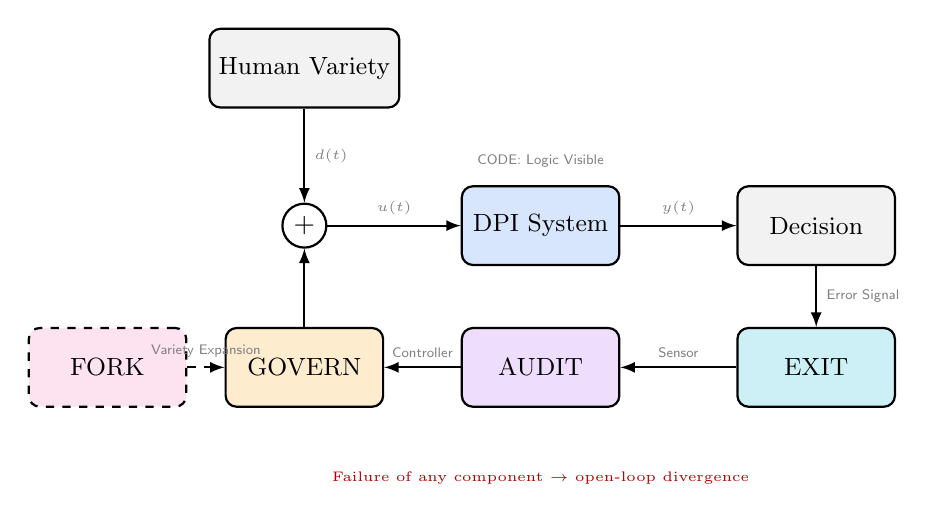
\begin{tikzpicture}[
    node distance=1.6cm, auto, >=latex, thick,
    block/.style={draw, rectangle, minimum height=1cm, minimum width=2cm, rounded corners, font=\small},
    sum/.style={draw, circle, inner sep=2pt},
    label/.style={font=\tiny\sffamily, text=gray}
]
    % Main flow
    \node[block, fill=gray!10] (disturbance) at (0, 2) {Human Variety};
    \node[sum] (sum1) at (0, 0) {$+$};
    \node[block, fill=codecolor!20] (plant) at (3, 0) {DPI System};
    \node[block, fill=gray!10] (output) at (6.5, 0) {Decision};

    % Feedback path
    \node[block, fill=exitcolor!20] (exit) at (6.5, -1.8) {EXIT};
    \node[block, fill=auditcolor!20] (audit) at (3, -1.8) {AUDIT};
    \node[block, fill=governcolor!20] (govern) at (0, -1.8) {GOVERN};

    % FORK as expansion
    \node[block, fill=forkcolor!20, dashed] (fork) at (-2.5, -1.8) {FORK};

    % CODE overlay
    \node[label, above=0.1cm of plant] {CODE: Logic Visible};

    % Connections - forward path
    \draw[->] (disturbance) -- node[right, label] {$d(t)$} (sum1);
    \draw[->] (sum1) -- node[above, label] {$u(t)$} (plant);
    \draw[->] (plant) -- node[above, label] {$y(t)$} (output);

    % Connections - feedback path
    \draw[->] (output) -- node[right, label] {Error Signal} (exit);
    \draw[->] (exit) -- node[above, label] {Sensor} (audit);
    \draw[->] (audit) -- node[above, label] {Controller} (govern);
    \draw[->] (govern) -- (sum1);

    % FORK expansion
    \draw[->, dashed] (fork) -- node[above, label] {Variety Expansion} (govern);

    % Annotations
    \node[font=\tiny, text=red!70!black, align=center] at (3, -3.2) {Failure of any component $\rightarrow$ open-loop divergence};
\end{tikzpicture}
\caption{\textbf{Corrigibility as a Closed-Loop Control Architecture.} Digital Public Infrastructure is modeled as a feedback control system subject to continuous human and environmental disturbance. Corrigibility requires that error signals (EXIT) remain detectable, that system behavior be intelligible (CODE), that sensing mechanisms be transparent (AUDIT), that binding corrective authority exist (GOVERN), and that structural reproduction be feasible (FORK). Failure of any single component collapses the loop into open-loop operation. Under non-zero integrating disturbance, error diverges unboundedly (Null-Feedback Instability Theorem, Appendix~\ref{appendix:proofs}). Corrigibility is therefore a structural property of loop integrity, not a matter of operator intent.}
\label{fig:control-loop}
\end{figure}

\subsection{Test 1: EXIT (Reversibility of Participation)}

\begin{definition}[EXIT]
\label{def:exit}
A system $S$ satisfies \textbf{Reversibility of Participation} if, for any user in state $s \in S$, there exists a transition to a non-participatory state $s_0$ such that the penalty $\pi(s \to s_0)$ is strictly bounded: $\pi(s \to s_0) < \tau_{\text{exit}}$, where $\tau_{\text{exit}}$ is a threshold below which the penalty does not constitute material exclusion from essential services.
\end{definition}

The foundational condition of any corrigible system is the \textbf{Reversibility of Participation}. Irrevocable consent functions structurally as mandatory lock-in. For an infrastructure to operate as a public utility rather than a coercive instrument, users must possess the capacity to withdraw from it without incurring disproportionate penalty or material exclusion.

In practice, many systems operate as a ratchet. They are easy to enter but functional imperatives make them impossible to leave. \textbf{Aadhaar} exemplifies this failure: opting out results in exclusion from banking, food rations, and mobile connectivity. When a system becomes a prerequisite for existence, refusal results in a disproportionate survival penalty rather than functioning as feedback. \textbf{UPI} partially mitigates this because cash remains legal tender, but network effects increasingly marginalize non-participants. \textbf{Linux}, by contrast, imposes no survival penalty: a user can migrate to BSD or Windows without losing access to essential services.

From a cybernetic perspective, EXIT constitutes the primary negative feedback loop. Blocking this channel silences the user's error signal. This blockade overloads the political layer with demands that the technical layer has suppressed.

This dynamic was formalized by Hirschman \citep{hirschman1970} in his analysis of organizational decline. Hirschman distinguished two correction mechanisms: exit (withdrawal from participation) and voice (attempts to change the system from within). His central finding is that these mechanisms exist in productive tension, not as substitutes.

Exit, in Hirschman's formulation, is ``neat,'' ``impersonal,'' and ``indirect'': one either exits or one does not. This binary quality makes exit a high-bandwidth error signal. When users leave, the system receives unambiguous information that something has failed. Voice, by contrast, is costly and conditioned on the influence and bargaining power that participants can bring to bear. Voice is gradual, political, and requires sustained effort.

Critically, Hirschman demonstrated that exit without voice produces abandonment rather than correction: quality-conscious users flee rather than fight. But voice without exit produces capture: complaints become cosmetic (see Section~\ref{subsec:grievance}) because the system faces no credible threat of user departure. The effectiveness of voice depends on the credibility of exit.

This framework illuminates why mandatory enrollment is structurally pathological. By eliminating exit, a system does not merely suppress one feedback channel. It degrades voice itself. When citizens cannot leave, their complaints lack credibility. The operator can absorb infinite grievance without modifying system behavior ($\partial S / \partial G = 0$). Hirschman's insight formalizes what cybernetics predicts: blocking the error signal does not eliminate the error; it eliminates the system's capacity to respond.

\subsection{Test 2: CODE (Inspectability of Logic)}

\begin{definition}[CODE]
\label{def:code}
A system $S$ satisfies \textbf{Inspectability of Logic} if, for any decision function $f: X \to Y$ that determines user outcomes, there exists a publicly accessible artifact $A_f$ such that $A_f$ fully specifies the computation of $f(x)$ for all inputs $x \in X$. For learned systems, $A_f$ includes training data provenance, model architecture, and alignment procedures.
\end{definition}

Users who cannot leave a system must possess the ability to inspect it. \textbf{Inspectability of Logic} requires that the rules determining outcomes are visible to those they govern. Power in a digital system resides in execution. Lessig \citep{lessig2006} established that software architecture functions as regulation: code ``determines what people can or cannot do in the first place,'' unlike legal regulation which sets rules for behavior and retroactively punishes non-compliance. This is regulation without appeal. If the execution path remains hidden, that power is absolute; it is not merely unaccountable but structurally unobservable to those it governs.

Transparency specifications or open standards are insufficient if the executing artifact remains a black box. \textbf{Aadhaar's} CIDR (Central Identities Data Repository) is proprietary: the matching algorithm that determines identity cannot be examined. \textbf{UPI} publishes API specifications, but the NPCI switching logic remains closed. \textbf{Let's Encrypt} demonstrates the alternative: its CA software is fully open source, allowing anyone to audit the certificate issuance logic that secures web traffic. For learned systems, the challenge intensifies. \textbf{Llama} publishes inference weights but withholds training data composition and RLHF preferences. This is spec-as-source: you can run the model but cannot understand why it produces specific outputs.

\subsection{Test 3: AUDIT (Independent Verification)}

\begin{definition}[AUDIT]
\label{def:audit}
A system $S$ satisfies \textbf{Independent Verification} if any external party $P$, without requiring operator authorization, can measure the system's error rate $\epsilon_S$, verify compliance with stated specifications, and document failure modes in production environments. Formally: $\forall P: \text{Access}(P, \epsilon_S) = \text{true}$ without $\text{Authorize}(\text{Operator}, P)$.
\end{definition}

While inspection enables understanding, \textbf{Independent Verification} enables truth. This functions as the sensor in the cybernetic feedback loop. A system is verifiable only if external, permissionless actors can test its behavior, measure its error rates, and document its failure modes within production environments.

\begin{remark}[The Auditability Distinction]
The framework does not equate auditability with direct participation. AUDIT $\neq$ ``everyone audits''; AUDIT $=$ ``no one can prevent auditing.'' \textbf{Journalism analogy:} Not everyone investigates corruption. Democracy still depends on the \textit{possibility} of investigation. The problem today is not that auditors exist; operators can legally block them. The tradeoff is contestable expertise over unchallengeable authority, a defensible democratic position.
\end{remark}

Incorrigible systems typically capture this function. \textbf{UPI} permits RBI regulatory audits, but transaction-level verification requires NPCI authorization; independent researchers cannot measure failure rates or dispute resolution times. \textbf{Open-weights AI models} (Llama, Qwen, DeepSeek) selectively publish red-teaming results while blocking independent adversarial testing at scale. \textbf{Bitcoin} provides the counter-model: every transaction is independently verifiable by any node, and consensus is cryptographic proof. Similarly, \textbf{Let's Encrypt} publishes Certificate Transparency logs, making every issued certificate publicly auditable in real time.

The structural function of opacity is sensor failure. A system whose error rates cannot be independently measured cannot be regulated. The controller receives no signal about divergence from intended behavior. Under Ashby's Law, such a system will drift until external forces impose correction. Those forces, operating outside the technical loop, will impose correction through channels the system cannot anticipate or absorb. \citet{pasquale2015} describes this as a ``one-way mirror'' relationship, but the cybernetic translation is precise: asymmetric observability breaks the feedback loop at the sensing stage.

\subsection{Test 4: GOVERN (Constitutive Constraint)}

\begin{definition}[GOVERN]
\label{def:govern}
A system $S$ satisfies \textbf{Constitutive Constraint} if there exists a governance function $G: \text{Rules} \to \text{Rules}'$ such that (1) $G$ is accessible to affected parties, not solely the operator; (2) $G$ is binding, meaning the operator cannot override $G$'s output; and (3) there exists a cryptographic or legal chain of custody linking system behavior to $G$'s constraints.
\end{definition}

Verification identifies the error, while \textbf{Constitutive Constraint} enforces the correction. This framework distinguishes structural governance from administrative functions like consultation, multi-stakeholder meetings, or feedback forms.

Governance exists only when binding constraints limit system behavior in ways the operator cannot override. \textbf{Aadhaar} is governed by UIDAI fiat: the same entity that operates the system sets its rules. \textbf{UPI} has NPCI governance, but NPCI is majority-owned by participating banks, creating structural conflicts. \textbf{Let's Encrypt} shows what binding constraint looks like: the ISRG charter legally binds the organization to its public benefit mission, with community board representation. \textbf{Bitcoin's} BIP process demonstrates governance through proven fork history; contentious changes have been rejected by the network, proving the community can override developer intent. \textbf{PostgreSQL's} contributor agreement prevents any single entity from capturing the project.

\subsubsection{The Post-Execution Fallacy}
A critical failure in modern policy involves relying on exogenous or post-hoc remedies to substitute for structural constraints. Mechanisms such as courts, ombudsmen, and grievance redressal officers operate on ``bureaucratic time,'' measured in months or years. Infrastructure operates on ``digital time,'' measured in milliseconds. A system that executes a harmful action, such as wrongful deletion of a beneficiary, and relies on a court order to reverse it six months later is structurally ungoverned for that duration. True governance must function within the system's execution loop to block prohibited states before they manifest.

Consequently, claims of governance must be evidentiary rather than declarative. They require a signed cryptographic chain of custody linking the operator's authority to an external, non-overrideable instrument.

\subsubsection{Strategic Openness vs Structural Accountability}

Open artifacts do not guarantee open governance. Systems can deploy \textit{asymmetric openness}: releasing code or weights for ecosystem adoption while retaining governance control. This pattern (detailed in Section~\ref{sec:diagnosis}) satisfies CODE while failing GOVERN. The GOVERN test requires bidirectional accountability: not merely that citizens can observe the system, but that they can correct it. A system that publishes its code while reserving all governance decisions to the operator has satisfied CODE but failed GOVERN.

A related confusion conflates governing one's own data with governing the system itself. Data protection frameworks (GDPR, CCPA) grant users rights to access, correct, delete, and port their data. These rights are necessary but insufficient: they allow users to manage information within rules the operator defines, not to change those rules. The GOVERN test asks: can affected parties change the rules, not merely operate within them?

\subsection{Test 5: FORK (Independent Reproduction)}

\begin{definition}[FORK]
\label{def:fork}
A system $S$ satisfies \textbf{Independent Reproduction} if an independent party can instantiate a functionally equivalent system $S'$ such that (1) no legal prohibition prevents $S'$'s deployment; (2) the artifacts required for reproduction (code, schemas, protocols) are publicly available; and (3) user state $U_S$ is portable: $U_S \to U_{S'}$. Natural barriers (capital, network effects) do not disqualify FORK; only constructed barriers (legal prohibition, regulatory monopoly) do.
\end{definition}

The ultimate check on power is the ability to recreate it. \textbf{Independent Reproduction} determines whether the ecosystem allows the infrastructure itself to be separated from its current steward. This requirement distinguishes structural resilience from simple market competition.

\begin{remark}[Credible Replaceability]
The paper does not define FORK as ``routine divergence in production.'' It defines FORK as \textbf{credible replaceability in extremis}. \textbf{Constitutional analogy:} The US Constitution is forkable (amendable, secession historically possible). That does not mean every county runs a different constitution. The \textit{possibility} disciplines the center. \textbf{The stable equilibrium:} Latent forkability + strong coordination incentives. Email works not because everyone forks SMTP, but because anyone \textit{could}. \textbf{Key asymmetry:} FORK is a threat, not a preference. No one wants fragmentation. But irreversibility without exit is worse.
\end{remark}

The existence of competitors, such as choosing between two proprietary cloud providers, provides an ``Exit'' option but not a ``Fork.'' Shifting providers allows a user to escape a specific operator, but it forces them to abandon their history, identity, and operational logic. This action is substitution, not reproduction.

\subsubsection{Natural vs Constructed Barriers}

A critical distinction must be drawn between barriers to forking that are \textbf{natural} (arising from coordination costs, network effects, or capital requirements) and those that are \textbf{constructed} (arising from legal prohibition, regulatory monopoly, or deliberate technical enclosure).

\begin{itemize}
    \item \textbf{Natural barriers}: Gmail dominates email not because forking SMTP is illegal, but because Google invested in spam filtering and UX. Anyone \textit{can} run their own mail server. Network effects and capital create friction, but not prohibition.
    \item \textbf{Constructed barriers}: NPCI is the \textit{only permitted} instant payment switch in India. The barrier is regulatory, not economic. Even with infinite capital, you cannot legally compete with UPI's core switching function.
    \item \textbf{Grant-conditioned barriers}: Sri Lanka's MOSIP implementation is contractually restricted to donor-country system integrators, despite MOSIP's open-source license \citep{biometricupdate2025}. The barrier is neither regulatory nor technical but financial: grant conditions foreclose supplier choice, demonstrating how ``open'' DPI exports can create new dependencies.
\end{itemize}

The FORK test fails only when constructed barriers prevent reproduction. Natural barriers reduce the \textit{likelihood} of forking; constructed barriers eliminate its \textit{possibility}. A system with high natural barriers but no constructed barriers (Linux, email) remains structurally corrigible. A system with low natural barriers but constructed prohibition (hypothetically: open-source software banned by law) would fail FORK despite technical simplicity.

\subsubsection{State Portability as a Precondition for Fork}

A critical structural requirement: code forkability is insufficient if \textbf{user state} is non-transferable. In traditional software (Linux, PostgreSQL), the artifact being forked \textit{is} the system. In Digital Public Infrastructure, the artifact is merely the skeleton; the system includes the user's credentials, transaction history, social graph, and accumulated trust relationships.

Let $U_S$ denote the user state graph in system $S$, and $S'$ a forked alternative. A fork is \textbf{functionally meaningful} only if:

\begin{equation}
U_S \to U_{S'} \quad \text{(state portability)}
\label{eq:state-portability}
\end{equation}

Open code with locked data produces a hollow fork. The legal right to reproduce an identity system is meaningless if citizens cannot port their credentials, attestations, and service eligibility to the new instance.

\paragraph{Switching Cost and Portability.} The practical barrier to exit and fork can be assessed through \textbf{switching cost}: the aggregate friction of data export, service downtime, credential re-establishment, network loss, and legal barriers. When switching cost to all plausible alternatives exceeds a policy threshold, EXIT and FORK functionally fail regardless of formal rights. Aadhaar exhibits near-maximal switching cost: no data export exists, service denial during transition is total, and legal mandate forecloses alternatives. UPI retains lower switching cost because cash and cards remain legal. The formal operationalization appears in Appendix~\ref{appendix:proofs}.

\paragraph{Technical Requirements for Portability.} To ensure meaningful forkability, DPI systems must implement: (1) standardized export bundles with user-owned credentials, (2) interoperability APIs to accept ported data, and (3) statutory guarantees requiring public services to accept verified portable credentials. This is the lesson of PSD2 in banking: portability mandates made bank-switching economically viable.

A system passes the FORK test only if the community possesses the legal rights, technical artifacts, economic means, \textbf{and state portability guarantees} to spawn a functionally equivalent instance. \textbf{Aadhaar} fails completely: no entity outside UIDAI can reproduce the identity infrastructure. \textbf{OpenSearch} demonstrates what successful forking looks like. When Elastic changed its license, AWS forked Elasticsearch and the community continued development independently. \textbf{Linux} has been forked thousands of times (Android, Chrome OS, countless distributions). \textbf{Llama} presents partial forkability: anyone can run the weights, but reproducing the training requires resources only a handful of companies possess. If Meta abandoned Llama tomorrow, the community could not recreate it.

\begin{table}[htbp]
\centering
\begin{tabular}{@{}lllp{5.5cm}@{}}
\toprule
\textbf{System} & \textbf{EXIT} & \textbf{FORK} & \textbf{Structural Reality} \\
\midrule
Cloudflare & PASS & FAIL & Can switch to Fastly, cannot reproduce \\
AWS & PASS & FAIL & Can migrate to Azure, logic/state locked \\
Aadhaar & FAIL & FAIL & Cannot refuse, cannot reproduce \\
Linux & PASS & PASS & Can leave, can fork \\
Llama & PASS & PARTIAL & Can run weights, cannot reproduce training \\
\bottomrule
\end{tabular}
\caption{Differentiation between Exit (Substitution) and Fork (Reproduction)}
\end{table}

\subsection{The Topology of Necessity}

Five tests describe the anatomy of a stable control loop rather than a random assortment of normative virtues (see Figure~\ref{fig:topology}).

\begin{itemize}[noitemsep,topsep=0pt]
    \item \textbf{EXIT} provides the Error Signal.
    \item \textbf{AUDIT} acts as the Sensor.
    \item \textbf{CODE} ensures Transmission Clarity.
    \item \textbf{GOVERN} serves as the Actuator.
    \item \textbf{FORK} provides Selection Pressure over the entire loop.
\end{itemize}

Failure in any single dimension breaks the control loop at a specific physical point. The result is not partial infrastructure but \textbf{Open Loop Control}. An open-loop system executes directives without the capacity to sense deviation, interpret error, or apply corrective force.

Under conditions of human variety and environmental change, open-loop control is structurally unstable. Error accumulates without bound. Misalignment compounds. The system drifts toward failure.

Corrigibility is the structural precondition that closes the loop. Only when all five tests are satisfied does a system possess a complete feedback topology capable of detecting divergence, transmitting intelligible signals, executing correction, and replacing failed control logic when necessary. Without this closure, stability is mathematically and operationally impossible.

\begin{figure}[H]
\centering
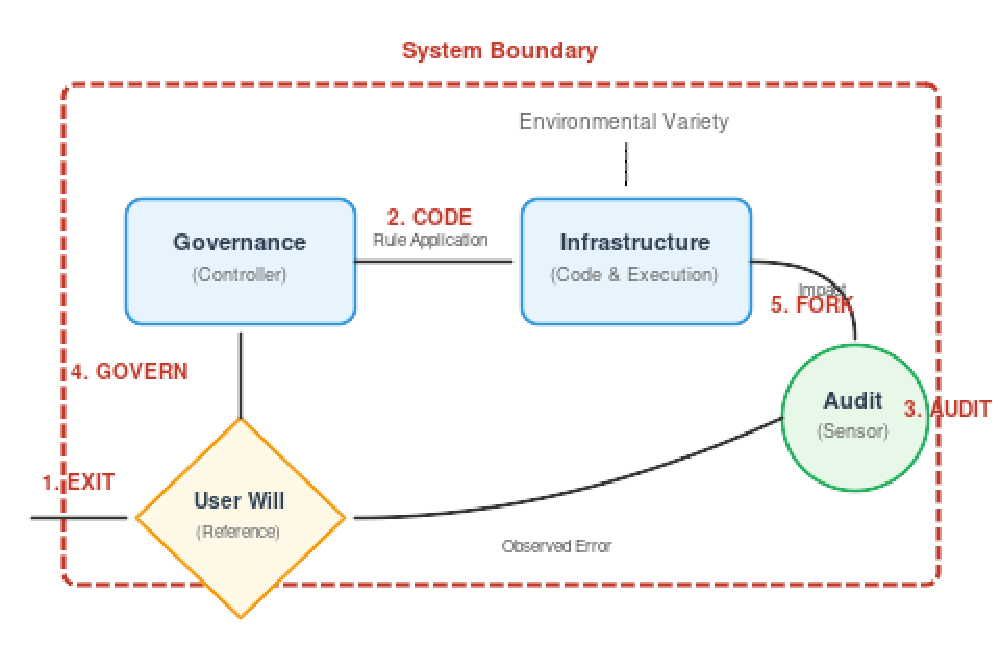
\includegraphics[width=0.75\textwidth]{figures/topology-of-necessity.pdf}
\caption{\textbf{Topology of Necessity.} Each corrigibility test corresponds to a breakage point in the feedback control loop.}
\label{fig:topology}
\end{figure}

\begin{figure}[H]
\centering
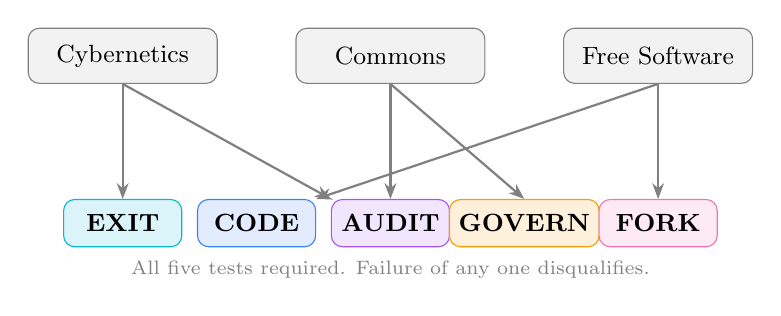
\begin{tikzpicture}[scale=0.85,
    tradition/.style={rectangle, rounded corners, draw=gray, fill=gray!10, minimum width=2.4cm, minimum height=0.7cm, font=\small},
    test/.style={rectangle, rounded corners, draw=#1, fill=#1!15, minimum width=1.5cm, minimum height=0.6cm, font=\small\bfseries},
    arrow/.style={-{Stealth[length=2mm]}, gray, thick}
]
% Three traditions at top
\node[tradition] (cyber) at (0,2.5) {Cybernetics};
\node[tradition] (commons) at (4,2.5) {Commons};
\node[tradition] (foss) at (8,2.5) {Free Software};

% Five tests at bottom
\node[test=exitcolor] (exit) at (0,0) {EXIT};
\node[test=codecolor] (code) at (2,0) {CODE};
\node[test=auditcolor] (audit) at (4,0) {AUDIT};
\node[test=governcolor] (govern) at (6,0) {GOVERN};
\node[test=forkcolor] (fork) at (8,0) {FORK};

% Connections - Cybernetics
\draw[arrow] (cyber.south) -- (exit.north);
\draw[arrow] (cyber.south) -- (audit.north west);

% Connections - Commons
\draw[arrow] (commons.south) -- (audit.north);
\draw[arrow] (commons.south) -- (govern.north);

% Connections - FOSS
\draw[arrow] (foss.south) -- (code.north east);
\draw[arrow] (foss.south) -- (fork.north);

% Labels
\node[font=\scriptsize, gray] at (4,-0.7) {All five tests required. Failure of any one disqualifies.};
\end{tikzpicture}
\caption{Five corrigibility tests derived from three independent theoretical traditions.}
\label{fig:framework}
\end{figure}

\subsection{Structural Symmetry of Power}

The five tests, while derived from distinct intellectual traditions, share a common organizing principle. Each enforces a constraint on power concentration at a different layer of the system. Together, they form a single power invariant:

\begin{center}
\begin{tabular}{@{}lll@{}}
\toprule
\textbf{Layer} & \textbf{Test} & \textbf{Function (Cybernetic)} \\
\midrule
Individual & EXIT & Reversibility of participation \\
Logic & CODE & Inspectability of rules \\
Logic & AUDIT & Verifiability of error \\
System & GOVERN & Constraint on controller variance \\
Ecosystem & FORK & Selection pressure via reproduction \\
\bottomrule
\end{tabular}
\end{center}

Each test enforces the same principle: \textit{No actor exercising power may be the sole judge of its continuation, scope, or correction.}

A system without EXIT is coercive. A system without GOVERN is arbitrary. A system without FORK is captive.

\subsection{Layer-Decomposed Evaluation}
\label{subsec:layers}

Complex infrastructure frequently stratifies into distinct functional layers, each with independent governance, transparency, and reproducibility properties. The five tests must be applied to each layer separately when:

\begin{enumerate}[noitemsep,topsep=0pt]
    \item Different entities control different layers (protocol versus implementation versus trust framework)
    \item Transparency varies across layers (open protocol, closed switching logic)
    \item Forkability differs by layer (code is forkable, network effects are not)
\end{enumerate}

\subsubsection{Propagation Rule}

A system that passes a test at one layer but fails at another does not achieve ``partial'' compliance. It fails the test. The evaluation proceeds from the layer closest to user impact upward; failure at any layer propagates to the whole.

Formally: Let $L_1, L_2, \ldots, L_n$ be the layers of a system, ordered by proximity to user impact. For test $T$:

\begin{equation}
T_{\text{system}} = \bigwedge_{i=1}^{n} T(L_i)
\label{eq:layer-propagation}
\end{equation}

The system passes $T$ if and only if every layer passes $T$. The full corrigibility determination extends this across all five tests:

\begin{equation}
\text{Corrigible}(S) = \bigwedge_{t \in \mathcal{T}} \bigwedge_{i=1}^{n} T_t(L_i) \quad \text{where } \mathcal{T} = \{\text{EXIT, CODE, AUDIT, GOVERN, FORK}\}
\label{eq:full-corrigibility}
\end{equation}

This double conjunction formalizes the ``weakest link'' principle: failure of any test at any layer propagates to the system determination.

\subsubsection{Application to Identity Infrastructure}

\begin{table}[htbp]
\centering
\small
\begin{tabular}{@{}llp{5cm}@{}}
\toprule
\textbf{Layer} & \textbf{Example Components} & \textbf{Typical Failure Mode} \\
\midrule
Protocol & W3C DID, VC Data Model & Often passes CODE \\
Implementation & Specific resolver, wallet software & May fail CODE (proprietary) \\
Credential & Issuer policies, attribute schemas & Often fails GOVERN (unilateral issuer) \\
Trust & Relying party acceptance, trusted lists & Often fails FORK (cannot reproduce acceptance) \\
\bottomrule
\end{tabular}
\caption{Identity infrastructure layer decomposition}
\label{tab:identity_layers}
\end{table}

The UPI payment rail exhibits similar layering: the protocol specification (NPCI-published) passes CODE at the protocol layer, but the switching logic (NPCI-operated) fails CODE at the implementation layer. Since the implementation layer is closer to user impact, the system fails CODE.

\subsubsection{The Weakest-Layer Principle}

This propagation rule has a counterintuitive but structurally necessary consequence: a system's corrigibility status equals its weakest layer across any test dimension. Strength at one layer cannot compensate for failure at another.

This principle prevents a common evasion: claiming corrigibility by publishing peripheral artifacts while retaining control over the layers that determine outcomes. Open-washing (Section~\ref{subsec:openwashing}) typically exploits layer confusion. Releasing SDKs (passing CODE at the interface layer) while keeping core logic proprietary (failing CODE at the execution layer) does not produce partial corrigibility. It produces total failure at the execution layer, which propagates to the system determination.

%% ============================================
%% SECTION 5: EMPIRICAL EVALUATION
%% ============================================

\section{Empirical Evaluation}
\label{sec:diagnosis}

The preceding sections established what corrigibility means and why it matters. Theory, however, must confront practice. Before analyzing \textit{why} systems fail these tests (the political economy) or \textit{how} the tests apply to AI (the stress test), we first demonstrate \textit{that} they fail and document the human consequences. This section applies the five tests to real-world infrastructure, establishing the concrete stakes that motivate the theoretical extensions to follow.

To demonstrate the framework's application, we evaluate systems across three categories: government infrastructure promoted as ``DPI,'' platform infrastructure claiming ``openness,'' and infrastructure that satisfies all five tests.

\paragraph{A Note on Utility.} These evaluations assess structural accountability, not functional utility. A system can be simultaneously useful and incorrigible. Aadhaar may enable efficient service delivery; this does not establish that it permits correction by those it affects. The framework evaluates governance architecture, not operational performance. Utility and accountability are orthogonal dimensions: neither implies the other.

\subsection{Government Infrastructure: The Trap of Partial Compliance}

Government-operated systems currently designated as Digital Public Infrastructure frequently exhibit a dangerous failure mode: they achieve partial compliance on technical tests (EXIT, CODE, AUDIT) while failing structurally on governance tests (GOVERN, FORK). By capturing the monopoly on execution, they render the feedback loop inoperable.

\begin{table}[p]
    \centering
    \scriptsize
    \caption{\textbf{Evaluation of Government Infrastructure.} Centralized execution leads to consistent structural failure despite ``open standards'' rhetoric.}
    \label{tab:govt_infra}

    % -- Subtable A: Aadhaar --
    \begin{subtable}{1\textwidth}
        \centering
        \caption{Aadhaar (India): Mandatory ID}
        \begin{tabular}{@{}llp{7cm}@{}}
            \toprule
            \textbf{Test} & \textbf{Result} & \textbf{Evidence} \\
            \midrule
            EXIT & $\times$ & Disproportionate penalty: exclusion from PDS, banking, SIM \citep{khera2019}. \\
            CODE & $\times$ & Execution logic opaque: proprietary matcher, closed algorithms. \\
            AUDIT & $\times$ & External testing prohibited: independent error measurement illegal. \\
            GOVERN & $\times$ & No binding constraint: UIDAI is both operator and regulator. \\
            FORK & $\times$ & No legal/technical/economic means: total centralized capture. \\
            \bottomrule
        \end{tabular}
    \end{subtable}

    % -- Subtable B: UPI --
    \begin{subtable}{1\textwidth}
        \centering
        \caption{UPI (India): Payment Rail}
        \begin{tabular}{@{}llp{7cm}@{}}
            \toprule
            \textbf{Test} & \textbf{Result} & \textbf{Evidence} \\
            \midrule
            EXIT & \textcolor{orange}{PARTIAL} & Cash exists but network effects coerce. \\
            CODE & \textcolor{orange}{PARTIAL} & Protocol specs open, switching logic closed. \\
            AUDIT & \textcolor{orange}{PARTIAL} & Regulator audits, public measurement blocked. \\
            GOVERN & $\times$ & Banks own NPCI, regulate themselves. \\
            FORK & $\times$ & Hub-and-spoke requires NPCI cooperation. \\
            \bottomrule
        \end{tabular}
    \end{subtable}

    % -- Subtable C: Pix --
    \begin{subtable}{1\textwidth}
        \centering
        \caption{Pix (Brazil): Central Bank Payment}
        \begin{tabular}{@{}llp{7cm}@{}}
            \toprule
            \textbf{Test} & \textbf{Result} & \textbf{Evidence} \\
            \midrule
            EXIT & \textcolor{orange}{PARTIAL} & Cash/cards exist; digital-only services coerce. \\
            CODE & \textcolor{orange}{PARTIAL} & API spec public; central routing closed. \\
            AUDIT & \textcolor{orange}{PARTIAL} & Stats public; independent measurement blocked. \\
            GOVERN & $\times$ & BCB sets/enforces rules unilaterally. \\
            FORK & $\times$ & Central switch requires BCB. \\
            \bottomrule
        \end{tabular}
    \end{subtable}

    % -- Subtable D: X-Road --
    \begin{subtable}{1\textwidth}
        \centering
        \caption{X-Road (Estonia/Nordic): Data Exchange Layer}
        \begin{tabular}{@{}llp{7cm}@{}}
            \toprule
            \textbf{Test} & \textbf{Result} & \textbf{Evidence} \\
            \midrule
            EXIT & $\times$ & Exclusion from government services. \\
            CODE & $\checkmark$ & MIT source on GitHub. \\
            AUDIT & $\checkmark$ & Transaction logs, documented APIs. \\
            GOVERN & $\checkmark$ & NIIS treaty, MIT license irrevocable. \\
            FORK & $\checkmark$ & 25+ country deployments prove feasibility. \\
            \bottomrule
        \end{tabular}
    \end{subtable}

    % -- Subtable E: UK Open Banking --
    \begin{subtable}{1\textwidth}
        \centering
        \caption{UK Open Banking: Regulated API Standard}
        \begin{tabular}{@{}llp{7cm}@{}}
            \toprule
            \textbf{Test} & \textbf{Result} & \textbf{Evidence} \\
            \midrule
            EXIT & \textcolor{orange}{PARTIAL} & Can revoke API consent; cannot exit banking. \\
            CODE & $\times$ & Bank implementations proprietary. \\
            AUDIT & $\checkmark$ & FCA oversight, TPP certification. \\
            GOVERN & $\checkmark$ & CMA order, PSD2 regulation. \\
            FORK & \textcolor{orange}{PARTIAL} & Rights exist; means require regulatory approval. \\
            \bottomrule
        \end{tabular}
    \end{subtable}
\end{table}

\textbf{Pattern}: X-Road (4/5) fails only EXIT \citep{xroad2026}. UK Open Banking (2/5) passes AUDIT and GOVERN but fails CODE: the API \textit{specification} is public, but the bank \textit{implementations} are proprietary. Specification $\neq$ Code. You can see the interface; you cannot inspect the execution.

\subsection{Platform Infrastructure: The Illusion of Openness}

In the private sector, systems often leverage "open source" branding while retaining centralized control. This decoupling of artifact transparency from governance reality creates a distinct failure pattern: the artifacts are public; the decisions are not.

\begin{table}[htbp]
    \centering
    \scriptsize
    \caption{\textbf{Evaluation of Private/Platform Infrastructure.} Technical openness (Source/Weights) does not guarantee structural accountability.}
    \label{tab:corp_infra}

    % -- Subtable A: Open Weights AI --
    \begin{subtable}{1\textwidth}
        \centering
        \caption{Open-Weights AI (Llama, etc.)}
        \begin{tabular}{@{}llp{7cm}@{}}
            \toprule
            \textbf{Test} & \textbf{Result} & \textbf{Evidence} \\
            \midrule
            EXIT & $\checkmark$ & Can run locally, switch models freely. \\
            CODE & \textcolor{orange}{PARTIAL} & Weights public; training data/RLHF opaque. \\
            AUDIT & \textcolor{orange}{PARTIAL} & Black-box probing possible; lineage unverifiable. \\
            GOVERN & $\times$ & Firm sets safety/capability trade-offs unilaterally. \\
            FORK & \textcolor{orange}{PARTIAL} & Fine-tuning possible; retraining blocked by compute. \\
            \bottomrule
        \end{tabular}
    \end{subtable}

    % -- Subtable B: Android --
    \begin{subtable}{1\textwidth}
        \centering
        \caption{Android (AOSP + GMS)}
        \begin{tabular}{@{}llp{7cm}@{}}
            \toprule
            \textbf{Test} & \textbf{Result} & \textbf{Evidence} \\
            \midrule
            EXIT & \textcolor{orange}{PARTIAL} & Device portable; ecosystem lock-in creates friction. \\
            CODE & \textcolor{orange}{PARTIAL} & AOSP open; Play Services/Identity closed. \\
            AUDIT & \textcolor{orange}{PARTIAL} & OS auditable; Google Services opaque. \\
            GOVERN & $\times$ & Google sets roadmap/certification unilaterally. \\
            FORK & \textcolor{orange}{PARTIAL} & LineageOS exists; app ecosystem requires GMS. \\
            \bottomrule
        \end{tabular}
    \end{subtable}

    % -- Subtable C: Signal --
    \begin{subtable}{1\textwidth}
        \centering
        \caption{Signal Protocol}
        \begin{tabular}{@{}llp{7cm}@{}}
            \toprule
            \textbf{Test} & \textbf{Result} & \textbf{Evidence} \\
            \midrule
            EXIT & $\checkmark$ & Can switch to alternatives freely. \\
            CODE & $\checkmark$ & Client and server source available (GPL/AGPL). \\
            AUDIT & $\checkmark$ & Cryptographic properties independently verifiable. \\
            GOVERN & $\times$ & Foundation board sets direction unilaterally. \\
            FORK & $\times$ & No federation locks network effects. \\
            \bottomrule
        \end{tabular}
    \end{subtable}
\end{table}

\textbf{Pattern: Asymmetric Openness.} These systems deploy strategic openness: releasing artifacts for ecosystem capture while retaining governance. This satisfies CODE (inspection possible) while failing GOVERN (correction blocked). The framework distinguishes artifact transparency (can you see the code?) from governance accountability (can you correct the system?). Open weights, open protocols, and open standards can each mask closed correction loops. ``Open weights'' $\neq$ ``open.'' ``Open source'' $\neq$ ``accountable.'' The artifact is open. The correction loop is closed. Seeing the machine does not govern it.

\subsection{Corrigible Infrastructure}

For contrast, Table~\ref{tab:positive} summarizes eighteen systems that pass all five tests. A striking pattern emerges: these systems are predominantly non-essential infrastructure. No individual's survival depends on accessing Linux or Let's Encrypt. This correlation between corrigibility and non-essentiality is not coincidental; it reflects a structural tension analyzed later in this paper.

\begin{table}[htbp]
\centering
\small
\renewcommand{\arraystretch}{1.3}
\begin{tabular}{@{}l>{\raggedright}p{3.2cm}>{\centering\arraybackslash}p{1.2cm}p{5.8cm}@{}}
\toprule
\rowcolor{gray!15}
\textbf{System} & \textbf{Steward} & \textbf{Score} & \textbf{Why Corrigible} \\
\midrule
\rowcolor{green!8}
Linux Kernel & Linux Foundation & \textbf{5/5} & Fully reproducible. Full triad (legal, technical, economic) exists. Independent distributions prove forkability. \\
Let's Encrypt & ISRG & \textbf{5/5} & Open source CA, IETF standards, nonprofit 501(c)(3) \\
\rowcolor{green!8}
Wikipedia & Wikimedia Foundation & \textbf{5/5} & CC BY-SA content, public edit history, community RfC governance \\
Matrix Protocol & Matrix.org Foundation & \textbf{5/5} & Apache 2.0, federated by design, self-hostable \\
\rowcolor{green!8}
Bluesky (AT Protocol) & Bluesky PBC & \textbf{5/5} & MIT/Apache, portable DID identity, self-hostable PDS \\
PostgreSQL & PGDG & \textbf{5/5} & BSD-like license, public mailing lists, major forks exist \\
\rowcolor{green!8}
IPFS & Protocol Labs & \textbf{5/5} & MIT/Apache, public IPIP process, no token governance \\
Bitcoin & Decentralized & \textbf{5/5} & MIT source, public BIP process, proven forks (BCH, BSV) \\
\rowcolor{green!8}
Kubernetes & CNCF & \textbf{5/5} & Apache 2.0, KEP process, distributions (OpenShift, k3s) \\
Firefox & Mozilla Foundation & \textbf{5/5} & MPL 2.0, nonprofit manifesto, forks (LibreWolf, Tor Browser) \\
\rowcolor{green!8}
Apache HTTP & Apache Foundation & \textbf{5/5} & Apache 2.0 license, ASF governance, powers 30\% of web \\
Apache Kafka & Apache Foundation & \textbf{5/5} & Apache 2.0, KIP process public, Fortune 500 standard \\
\rowcolor{green!8}
OpenSearch & Linux Foundation & \textbf{5/5} & Forked from Elasticsearch; Apache 2.0, multi-vendor governance \\
Valkey & Linux Foundation & \textbf{5/5} & Forked from Redis; BSD license, community governance restored \\
\rowcolor{green!8}
Hyperledger & LF Decentralized Trust & \textbf{5/5} & Apache 2.0 framework; institutional deployments require separate evaluation \\
LibreOffice & Document Foundation & \textbf{5/5} & Forked from OpenOffice; LGPL/MPL, nonprofit governance \\
\rowcolor{green!8}
MariaDB & MariaDB Foundation & \textbf{5/5} & Forked from MySQL; GPL, foundation governance \\
Eclipse IDE & Eclipse Foundation & \textbf{5/5} & EPL 2.0, 386 member orgs, committer-led governance \\
\bottomrule
\end{tabular}
\caption{Infrastructure systems satisfying all five corrigibility tests. All systems demonstrate full EXIT, CODE, AUDIT, GOVERN, and FORK compliance.}
\label{tab:positive}
\end{table}

\textbf{Fork as Correction}: OpenSearch, Valkey, LibreOffice, and MariaDB demonstrate Ashby's Law in practice. Each emerged when governance variety collapsed: Oracle's Sun acquisition (2010) triggered LibreOffice and MariaDB; unilateral license changes triggered OpenSearch (2021) and Valkey (2024). The ecosystem restored requisite variety through forking.

The framework is governance-agnostic: corporate participation is not disqualifying. Kubernetes (CNCF), Hyperledger, and Let's Encrypt all have significant corporate involvement while passing all tests. The test is whether governance permits correction, not who participates.

\textbf{License vs. Governance}: Redis Ltd. added AGPLv3 in 2025, restoring open licensing. But license is orthogonal to governance. \textit{License} determines what you may do with code; \textit{governance} determines who decides what it becomes. Redis passes one; Valkey passes both.

\textbf{International Counterexample: Estonia's X-Road.} Estonia's X-Road architecture provides a counterexample demonstrating that scale does not necessitate centralized capture. Its federated data exchange model distributes control across institutional nodes, preserving CODE transparency (fully open-source, MIT license) and enabling institutional FORK at the implementation layer. While EXIT remains limited for certain core registries, the federated topology significantly reduces concentration coupling compared to monolithic architectures. X-Road has been adopted by Finland, Iceland, and deployed in over 20 countries, illustrating that corrigibility properties are architectural rather than cultural. The framework does not require cultural homogeneity or small population size; it requires federated governance that prevents single-point capture.

\subsection{The Taxonomy of Open-Washing}
\label{subsec:openwashing}

Systems that fail these structural tests frequently employ vocabulary to obscure their closure:
\begin{enumerate}
    \item \textbf{Standard-Washing}: Adopting open technical standards (like ISO/W3C) as proxy for governance accountability.
    \item \textbf{Open-Washing}: Releasing peripheral SDKs while keeping core execution logic proprietary.
    \item \textbf{Multilateral-Washing}: Using international endorsements (G20, WB) to substitute for technical auditability.
    \item \textbf{Safety-Washing}: Justifying opacity by claiming inspection poses a security risk.
    \item \textbf{Consent-Washing}: Obtaining formal consent under conditions of economic coercion.
    \item \textbf{DID-Washing}: Deploying decentralized identifiers without decentralized governance (see Section~\ref{subsubsec:didwashing}).
    \item \textbf{Climate-Washing}: Using environmental rhetoric to legitimize structural changes whose primary effects extend beyond genuine climate mitigation (see Section~\ref{subsubsec:climatewashing}).
\end{enumerate}

\subsubsection{DID-Washing: The Layer Confusion Problem}
\label{subsubsec:didwashing}

Decentralized Identifiers (DIDs) present a distinct challenge to corrigibility evaluation because they separate technical decentralization from governance decentralization across multiple architectural layers. The W3C DID Core 1.0 specification \citep{w3cdid2022} defines DIDs as ``globally unique identifiers'' that ``do not require a centralized registration authority.'' This technical claim is accurate. However, a system can implement DIDs at the identifier layer while retaining centralized control at every layer that determines actual utility.

Identity infrastructure comprises at least four functional layers, each with independent governance:

\begin{table}[htbp]
\centering
\small
\caption{DID infrastructure layers and typical corrigibility failures}
\label{tab:did_layers}
\begin{tabular}{@{}lp{5cm}p{5cm}@{}}
\toprule
\textbf{Layer} & \textbf{Function} & \textbf{Common Failure} \\
\midrule
Identifier & DID generation, resolution & Often passes CODE (open specs) \\
Credential & Issuer policies, attribute schemas & Often fails GOVERN (unilateral issuer) \\
Wallet & Storage, presentation, consent & Often fails FORK (vendor lock-in) \\
Reliance & Verifier acceptance, trust frameworks & Often fails EXIT (no alternative verifiers) \\
\bottomrule
\end{tabular}
\end{table}

A system may achieve decentralization at the identifier layer while remaining fully centralized at the credential, wallet, or reliance layers. Evaluating only the DID specification produces a false positive; evaluating the complete stack reveals the actual governance topology.

\paragraph{Example: EU Digital Identity Wallet.} The proposed EU Digital Identity Wallet framework implements DIDs for identifier generation. However, the credential layer is governed by member state authorities with unilateral issuance power; the wallet layer specifies certified applications with vendor approval requirements; and the reliance layer mandates acceptance by specified service providers. At the identifier layer: decentralized. At the governance layer: centralized state control mediated through a federated but non-forkable architecture.

The framework's response: evaluate each layer independently, then apply the Weakest-Layer Principle. A system's corrigibility equals its weakest layer. DID-washing exploits the gap between technical specification and governance reality.

\subsubsection{Climate-Washing: Environmental Rhetoric as Capture Vector}
\label{subsubsec:climatewashing}

Climate policy has become a vector for infrastructure capture. The rhetorical pattern is consistent: invoke environmental necessity to justify surveillance, mandate digital-only interfaces, or eliminate cash. This section documents specific instances where climate framing masks structural changes that the framework identifies as incorrigibility failures.

\paragraph{15-Minute Cities.} The urban planning concept of ``15-minute cities'' has been weaponized to justify geofencing and movement tracking. The original concept (amenities within 15 minutes of residence) implies no surveillance. The implementation variant (digital permits required to cross neighborhood boundaries, as trialed in Oxford) implies mandatory tracking infrastructure. The climate framing (reduce car trips) obscures the governance change (movement requires permission).

Under the framework: a system that requires digital permission to move fails EXIT (cannot opt out without forfeiting mobility). The climate benefit is orthogonal to the corrigibility failure.

\paragraph{Cash Elimination.} Multiple jurisdictions have proposed eliminating physical currency to ``reduce carbon footprint of money.'' The environmental claim is empirically contested (digital payment infrastructure has significant energy costs). The governance effect is uncontested: elimination of cash creates mandatory digital payment infrastructure with no EXIT option.

\paragraph{Carbon Tracking.} Personal carbon accounting systems propose linking identity infrastructure to consumption tracking. The stated purpose is behavioral nudging for sustainability. The structural effect is comprehensive consumption surveillance with no technical or legal mechanism for opting out while maintaining normal economic participation.

The framework's response: environmental goals do not constitute exemptions from corrigibility requirements. A surveillance system does not become corrigible because its stated purpose is ecological. The tests evaluate architecture, not intentions.

%% ============================================
%% SECTION 6: POLITICAL ECONOMY OF DIGITAL INFRASTRUCTURE
%% ============================================

\section{The Political Economy of Digital Infrastructure}
\label{sec:political-economy}

The empirical evaluation reveals a troubling pattern: systems that serve essential functions consistently fail the five tests, while systems that pass are predominantly non-essential. This section analyzes \textit{why} this pattern exists. The answer lies in the political economy of infrastructure: the temporal dynamics of correction, the structural tension between essentiality and accountability, and the trilemma facing states that attempt to build sovereign digital infrastructure at scale.

\subsection{The Dynamics of Incorrigibility}
\label{sec:dynamics}

The five tests define the static architecture of a corrigible system. However, infrastructure exists in time. When we apply these structural requirements to dynamic systems, three fundamental implications emerge regarding stability, energy conservation, and the rule of law. These principles explain why centralized grievance redressal mechanisms (the standard answer of bureaucracies to error) are mathematically insufficient to guarantee stability.

\subsection{The Harm Accumulation Principle}

A critical clarification is required regarding the framework's claims about incorrigible systems:

\begin{quote}
\textbf{Principle (Harm Accumulation):} Incorrigible systems accumulate harm until correction becomes catastrophic rather than incremental. The framework does NOT claim ``incorrigibility leads to collapse.'' It claims that \textbf{corrigibility is a precondition for a system to be meaningfully public.}
\end{quote}

This is ontological classification, not historical prediction. North Korea is stable, incorrigible, and not public in any meaningful sense, confirming rather than refuting the framework. Tyrannies can persist indefinitely while crushing their subjects. The system stabilizes; the humans do not.

\begin{remark}[The Core Claim]
Corrigibility is not a guarantee of justice. It is a guarantee that \textbf{injustice is contestable}.
\end{remark}

A prison can be stable. A prison can even be efficient. But it is not public. The framework draws this line.

\subsection{The Correction Velocity Inequality}
\label{subsec:velocity}

Stability in a cybernetic system is not merely a function of whether a correction path \textit{exists}, but of its \textit{latency} relative to error generation. A correction mechanism that is theoretically available (e.g., a court case or a legislative amendment) but slower than the rate of divergence creates a runaway failure state.

\begin{principle}[Temporal Stability Condition]
A system is corrigible only if the rate of effective correction exceeds the rate of error accumulation. Correction velocity has both a lower bound (preventing harm accumulation) and an upper bound (preventing manipulation). The formal treatment appears in Appendix~\ref{appendix:proofs}.
\end{principle}

\begin{remark}[The Thermodynamics of Due Process]
The framework does NOT argue for automated, instantaneous, or algorithmic governance. Constitutional democracy invented latency: bicameralism, judicial review, and evidentiary hearings. \textbf{Friction is not failure; friction is how minorities survive majorities.}

However, the timescale mismatch is a thermodynamic constraint, not a jurisdictional preference. A court operating on bureaucratic time cannot mathematically regulate an automated system propagating errors at digital speed. The framework criticizes the \textit{absence} of native technical constraints, not the \textit{latency} of human justice.
\end{remark}

Error is driven by environmental volatility: identity fraud tactics, software exploits, pandemics, or economic shocks. These phenomena tend to grow exponentially or appear in high-velocity impulse shocks. In contrast, centralized governance operates on \textbf{bureaucratic time} (months or years) while technical errors accumulate on \textbf{digital time} (milliseconds).

This timescale mismatch is an instance of the Collingridge Dilemma \citep{collingridge1980}: a double-bind in technology governance. Early in a technology's development, change is easy but the need for change cannot be foreseen (the information problem). Later, when impacts become clear, change has become expensive, difficult, and time-consuming because the technology is entrenched (the power problem).

Digital Public Infrastructure exhibits the Collingridge Dilemma in acute form. By the time exclusion effects are documented (starvation deaths, banking denials, welfare failures), a system may have achieved mandatory status. Correction now requires not merely technical modification but legal amendment, bureaucratic reorganization, and political will. The system's success in achieving scale has made it resistant to correction.

Corrigibility is the structural response to this dilemma: build the correction mechanisms before the need for correction is apparent. EXIT, CODE, AUDIT, GOVERN, and FORK are not remedies applied after failure; they are architectural features that must be present from deployment. A system without these features will eventually require correction but will lack the capacity to receive it.

This inequality explains the failure of the ``post-execution'' remedies discussed in Section 4.4. Mechanisms like ombudsmen or grievance redressal officers inherently operate at a lower bandwidth and higher latency than the systems they supervise. When the correction loop is thermodynamically too slow to manage the entropy of the environment, error accumulates in the system until it suffers catastrophic collapse. Corrigibility requires closing the gap between error generation and correction; this is only possible if correction logic operates within the technical loop (Test 4), not outside it.

\subsection{The Conservation of Correction Demand}

When a system fails to correct errors, the demand for correction does not evaporate. It transforms.

\begin{principle}[Conservation of Correction Demand]
For a given system state, the total pressure for correction is constant. Correction flows through designed channels (EXIT, GOVERN) or emergent channels (protest, litigation, hacks, grey markets, civil unrest). Operators can choose \textit{where} correction occurs; they cannot choose \textit{whether} it occurs.
\end{principle}

By suppressing EXIT (via mandatory laws) and blocking GOVERN (via executive fiat), authorities force correction demand into channels that are slower, costlier, and fundamentally more destabilizing to the social order. Corrigibility acts as a pressure relief valve that converts potential volatility into system evolution.

\subsubsection{Grievance Is Not Feedback}
\label{subsec:grievance}

A critical distinction: \textit{grievance} is not \textit{governance}. Many incorrigible systems act as ``roach motels'' for complaints. They allow unlimited feedback submission, but the system state remains invariant. Grievance channels that record dissatisfaction without binding mechanisms to modify execution do not constitute a feedback loop. They serve an aesthetic function, mimicking responsiveness while preserving rigidity. Under Ashby's Law, if the controller's response variety does not increase in response to signal, regulation has failed.

\subsubsection{Active Deception}
\label{subsec:active-deception}

A more severe pathology occurs when systems do not merely fail to correct errors but actively misrepresent their state or capabilities. We term this \textbf{Active Deception}: the systematic production of false signals that degrade the epistemic environment for external oversight.

Active Deception takes three forms:

\paragraph{1. Safety-Washing.} Systems that claim safety certifications, audits, or approvals that do not correspond to verifiable structural properties. A system may publish ``privacy by design'' documents while implementing opaque centralized logging; display compliance badges while blocking independent audit access; or cite ethics board oversight while exempting operational decisions from board review. The deception lies in the gap between representation and verifiable architecture.

\paragraph{2. Open-Washing.} Systems that claim openness while structurally foreclosing the rights that openness implies. Publishing inference code while withholding training data, weights, or RLHF preferences constitutes open-washing: it mimics CODE compliance while preventing meaningful reproduction (FORK). The term ``open'' has been systematically degraded through this practice, requiring the framework to specify \textit{structural} rather than \textit{nominal} criteria.

\paragraph{3. Audit Theatre.} Systems that permit nominal inspection while structurally preventing the inspector from detecting errors. This includes: providing read access to sanitized logs rather than raw execution traces; permitting audits only at pre-announced times; or granting access to components that do not determine actual behavior. The auditor observes a Potemkin system; the production system operates under different logic.

These pathologies share a common structure: they corrupt the feedback channel by injecting false negatives. When external observers receive signals indicating ``compliant,'' ``safe,'' or ``open,'' they rationally reduce oversight intensity. The deception is not merely a failure to inform but an active degradation of the correction system's sensor function.

Under the framework's cybernetic model, Active Deception constitutes a \textbf{sensor attack}: the deliberate corruption of the AUDIT channel to prevent the control loop from detecting deviation. Unlike passive incorrigibility (which merely blocks correction), Active Deception induces false confidence that accelerates divergence.

\subsection{The Structural Preconditions of Law}
\label{subsec:rule-of-ledger}

These dynamics have profound implications for constitutional review. Legal doctrines such as proportionality analysis, as established in \textit{Puttaswamy v. Union of India} \citep{puttaswamy2017}, presuppose that state intrusions can be measured, minimized, and remedied. However, as \citet{bhatia2019} argues, modern digital systems frequently violate the structural assumptions upon which these legal doctrines rest.

A court cannot apply proportionality review to a system whose execution is opaque (\textbf{CODE}). A legislature cannot remedy harm if the mechanism of harm is an irreversible digital transaction (\textbf{EXIT}). A regulator cannot oversee a system if they lack the technical capability to inspect it independent of the operator (\textbf{AUDIT}).

Where digital systems block these channels structurally, the rule of law becomes a legal fiction. External review mechanisms cannot function meaningfully if the internal architecture is designed to resist observation and modification. Therefore, \textbf{corrigibility} should be understood not merely as a technical specification, but as the \textit{evidentiary precondition} required for the law to take hold of the machine.

\subsubsection{The Rule of the Ledger}

Digital execution introduces a rival governance paradigm: the \textbf{Rule of the Ledger}, in which authority is exerted through synchronized, self-executing artifacts rather than mediated institutional processes. Under this paradigm, the technical capacity for instantaneous state change (account freezes, entitlement adjustments) can be embedded in the execution layer; the institutional channels of review (courts, ombudsmen, bicameral procedural delays) operate on distinct and much slower time scales. The consequence is \textbf{Universal Failure Propagation}: when identity, payment, and entitlement layers synchronize, a single erroneous state transition in one layer can automatically and immediately propagate penalties across other layers.

Two structural implications follow. First, doctrines that presuppose reversible administrative acts (proportionality, injunctive relief) are ipso facto disabled if the necessary observability and reversal primitives are not present within the technical loop (\textbf{CODE}, \textbf{AUDIT}, \textbf{GOVERN}). Second, legal remedies become performative unless they are accompanied by verifiable, machine-enforceable restraints (signed chains of authority, multi-party escrow of execution privileges, or pre-authorized blocking hooks that operate within the same temporal envelope as the ledger itself).

The Rule of the Ledger therefore reframes the law-infrastructure relationship: courts and regulators cannot simply be invoked later; corrigibility requires embedding evidentiary and counter-majoritarian restraints into the system's operational fabric. This is not a call for ``autonomous legal machines'' but for technical modes of constraint that render legal review materially possible rather than symbolic.

\subsection{The Sovereignty, Scale, and Neutrality Tension}
\label{subsec:trilemma}

The empirical pattern identified in Section~\ref{sec:diagnosis} suggests a recurring structural tension in state-operated digital infrastructure. Systems that achieve population-scale deployment under centralized sovereign control frequently exhibit diminished structural neutrality at the execution layer.

\begin{definition}[System Properties]
Let a Digital Public Infrastructure system $S$ exhibit the following properties:
\begin{itemize}[noitemsep]
    \item \textbf{Sovereignty ($So$)}: The state retains centralized control over standards, execution, routing logic, and data residency.
    \item \textbf{Scale ($Sc$)}: The system is mandatory or near-mandatory for population-level access to essential services.
    \item \textbf{Neutrality ($N$)}: The execution layer satisfies structural corrigibility. Specifically, affected parties retain enforceable capacity across EXIT, CODE, AUDIT, GOVERN, and FORK sufficient to prevent discriminatory or unilateral control.
\end{itemize}
\end{definition}

Neutrality here is not a moral descriptor. It denotes preservation of governance variety sufficient to prevent structural capture at the execution layer.

\begin{proposition}[Topology-Dependent Tension]
\label{prop:trilemma}
Under centralized enforcement topology, a system that strongly maximizes both Sovereignty and Scale will experience compression of governance variety sufficient to place Neutrality at structural risk.
\end{proposition}

\textbf{Control-Theoretic Reasoning.} Under Ashby's Law, stability requires that controller variety meet or exceed environmental variety: $V_{\text{controller}} \geq V_{\text{environment}}$. In large-scale population systems, environmental variety increases with scale ($V_{\text{env}} \propto Sc$). Centralized sovereign control concentrates execution authority into a bounded institutional set, constraining governance variety. When scale increases while governance remains centralized, the ratio of corrective capacity to environmental complexity declines. Under centralized enforcement, governance capacity tends to scale sublinearly relative to environmental complexity (formal proof in Appendix~\ref{appendix:neutrality}).

The neutrality condition can be stated as:
\begin{equation}
V_{\text{eff}} \geq \theta \cdot V_{\text{env}}
\label{eq:neutrality-condition}
\end{equation}
where $V_{\text{eff}}$ is effective governance variety and $\theta \in (0,1]$ is a stability sufficiency constant. Neutrality degradation risk emerges when this condition fails.

\begin{figure}[htbp]
\centering
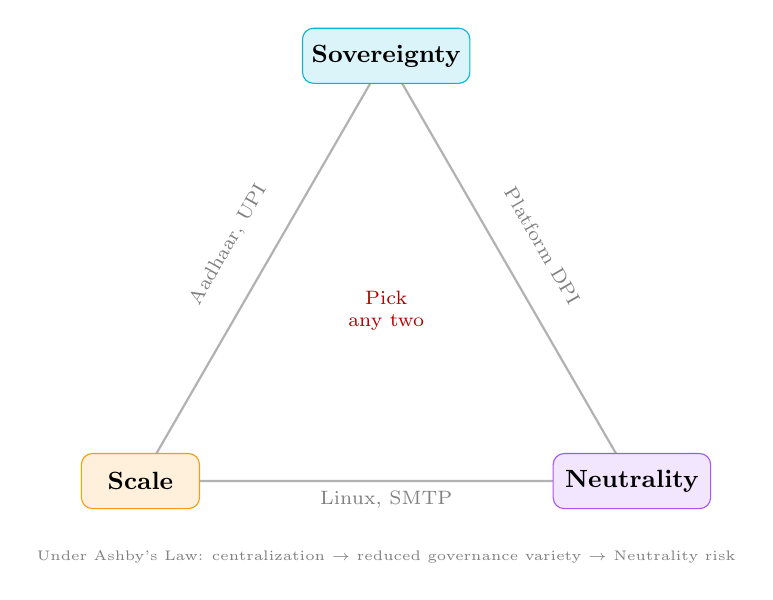
\begin{tikzpicture}[scale=1.2, font=\sffamily]
    % Triangle vertices
    \coordinate (S) at (0,3);      % Sovereignty (top)
    \coordinate (Sc) at (-2.6,-1.5);  % Scale (bottom left)
    \coordinate (N) at (2.6,-1.5);   % Neutrality (bottom right)

    % Draw triangle edges with labels
    \draw[thick, gray!60] (S) -- (Sc) -- (N) -- cycle;

    % Vertex labels with boxes
    \node[rectangle, rounded corners, draw=exitcolor, fill=exitcolor!15, minimum width=2cm, minimum height=0.7cm, font=\small\bfseries] at (S) {Sovereignty};
    \node[rectangle, rounded corners, draw=governcolor, fill=governcolor!15, minimum width=1.5cm, minimum height=0.7cm, font=\small\bfseries] at (Sc) {Scale};
    \node[rectangle, rounded corners, draw=auditcolor, fill=auditcolor!15, minimum width=2cm, minimum height=0.7cm, font=\small\bfseries] at (N) {Neutrality};

    % Edge labels showing what you get when you pick two
    \node[font=\scriptsize, text=gray, rotate=60, anchor=south] at (-1.5,0.9) {Aadhaar, UPI};
    \node[font=\scriptsize, text=gray, anchor=north] at (0,-1.5) {Linux, SMTP};
    \node[font=\scriptsize, text=gray, rotate=-60, anchor=south] at (1.5,0.9) {Platform DPI};

    % Center label
    \node[font=\scriptsize, text=red!70!black, align=center] at (0,0.3) {Pick\\any two};

    % Ashby annotation
    \node[font=\tiny, text=gray, align=center] at (0,-2.3) {Under Ashby's Law: centralization $\rightarrow$ reduced governance variety $\rightarrow$ Neutrality risk};
\end{tikzpicture}
\caption{\textbf{The Sovereignty, Scale, and Neutrality Tension.} Under centralized enforcement, states face structural pressure when optimizing for Sovereignty and Scale simultaneously. India Stack optimizes for Sovereignty + Scale with elevated Neutrality risk. Federated systems (Linux, SMTP) achieve Neutrality + Scale through distributed governance.}
\label{fig:trilemma}
\end{figure}

\textbf{Clarification: This Is Not an Impossibility Theorem.} The proposition does not assert that Sovereignty, Scale, and Neutrality are logically incompatible. It asserts that under centralized enforcement architecture, maximizing Sovereignty and Scale reduces governance variety unless compensatory mechanisms are introduced. The tension is architectural, not metaphysical. Neutrality can be preserved under Scale and Sovereignty if governance variety is restored through structural mechanisms such as federated execution, multi-issuer mandates, Functional Exit Equivalence (Section~\ref{subsubsec:fee}), state portability guarantees, or non-exclusive procurement rules.

\textbf{Workflow Capture Extension.} Workflow capture reduces effective corrective variety. Formally, effective governance capacity is suppressed as WCC (Workflow Capture Coefficient) increases (see Appendix~\ref{appendix:neutrality}). Thus, even when restoration mechanisms exist, high workflow capture reintroduces neutrality risk.

India's experience instantiates this constraint: the architectural choices that achieved sovereign control and near-universal coverage produced structural dependency on a small set of switching and credentialing authorities. That dependency compressed the correction channel's bandwidth, manifesting as the GOVERN failures documented in Table~\ref{tab:govt_infra}. The tension reframes these outcomes: the observed compression of corrective bandwidth is not an implementation mistake but a predictable consequence of architectural choice.

\begin{table}[htbp]
\centering
\small
\caption{Comparative topology and neutrality risk}
\label{tab:topology-risk}
\begin{tabular}{lccc}
\toprule
\textbf{Topology} & \textbf{Sovereignty} & \textbf{Scale} & \textbf{Neutrality Risk} \\
\midrule
Centralized Sovereign Stack & High & High & Elevated \\
Federated Protocol Model & Medium & High & Lower \\
Market Platform Model & Low (State) & High & Variable \\
Open Commons Model & Low & Medium & Low \\
\bottomrule
\end{tabular}
\end{table}

Any prescriptive response must therefore treat neutrality as an architectural variable (portability, multi-issuer requirement, anti-exclusive procurement), not an aspirational outcome. The Functional Exit Equivalence remedies in Section~\ref{subsubsec:arch-responses} address precisely this constraint.

\subsection{The Essential Services Problem}
\label{subsec:essential}

A pattern emerges from the preceding analysis: systems that pass all five tests are disproportionately non-essential infrastructure. Linux, PostgreSQL, Kubernetes, and Let's Encrypt power critical operations, but no individual's survival depends on accessing them. The systems promoted as DPI, which mediate access to food, banking, healthcare, and mobility, consistently fail.

This correlation reflects a structural tension between essentiality and corrigibility.

\begin{proposition}[Essentiality-Corrigibility Tension]
\label{prop:essentiality}
For any infrastructure system $S$ where participation is a prerequisite to survival, the EXIT test cannot be satisfied.
\end{proposition}

\begin{proof}
EXIT requires that refusal incur no disproportionate penalty (Section~\ref{sec:tests}, Test 1). Let $S$ be essential: participation is required for access to food, shelter, healthcare, or legal identity. Refusal of $S$ therefore entails exclusion from survival necessities. Exclusion from survival necessities is a disproportionate penalty by any reasonable standard. Therefore, EXIT fails. \qed
\end{proof}

This proposition formalizes the empirical observation: among the systems evaluated, those that pass all five tests are precisely those where participation remains genuinely voluntary.

\begin{corollary}[No Exemptions from Essentiality Tension]
The following do NOT constitute valid exemptions from Proposition~\ref{prop:essentiality}:
\begin{enumerate}[noitemsep]
    \item \textbf{Emergency necessity}: Pandemics, wars, and crises do not suspend the requirement for correction channels. Systems deployed under emergency conditions that block EXIT remain incorrigible; the emergency explains but does not justify the structural failure.
    \item \textbf{Efficiency gains}: That a mandatory system delivers services faster or cheaper than alternatives does not restore EXIT. Efficiency is orthogonal to corrigibility.
    \item \textbf{Democratic authorization}: Legislative mandates do not convert incorrigible systems into corrigible ones. A democratically enacted prison is still a prison.
    \item \textbf{Benevolent intent}: Good-faith operation does not substitute for structural accountability. The framework evaluates architecture, not intentions.
\end{enumerate}
\end{corollary}

\subsubsection{The Essentiality Trap}

Essential services create the economic coercion that undermines EXIT. When refusal means exclusion from survival, the feedback loop breaks regardless of other properties. \citet{hirschman1970} observed that exit is effective precisely because it is voluntary. The credible threat of departure disciplines the system. When departure means death (literal or social), exit ceases to function as feedback. It becomes self-exclusion.

The systems in Table~\ref{tab:positive} avoid this trap because alternatives exist. A developer who dislikes the Linux kernel's direction can migrate to BSD without losing the ability to compute. A journalist who distrusts Let's Encrypt can obtain certificates elsewhere. The existence of functional alternatives preserves the error signal.

Aadhaar has been made prerequisite to existence. Documented cases demonstrate the consequence: the Right to Food campaign documented 57 starvation deaths across nine Indian states between 2015 and 2018, with at least 19 directly attributed to Aadhaar-related exclusion from food rations \citep{khera2017}. These deaths are not anomalies; they are the structural prediction of a system that blocks EXIT while governing essential services.

\subsubsection{Functional Exit Equivalence (FEE)}
\label{subsubsec:fee}

When an infrastructure is essential for survival, literal exit is impossible. However, the cybernetic purpose of EXIT is not departure itself; it is the generation of a credible error signal. Essential systems must therefore implement \textbf{Functional Exit Equivalence (FEE)}: architectural guarantees that recreate the error-signal strength of market exit without requiring citizens to abandon society.

FEE is achieved structurally through three combined mechanisms:
\begin{enumerate}[noitemsep]
    \item \textbf{Multi-Issuer Mandates:} Procurement requires at least two legally independent credential issuers (preventing single-point capture).
    \item \textbf{Acceptance Diversity:} Public services must accept federated credential classes, as demonstrated by the multi-national deployment of X-Road.
    \item \textbf{Protected Statutory Fallbacks:} The legal guarantee of non-digital analogues.
\end{enumerate}

The demand for FEE is not a regressive desire to maintain paper ledgers indefinitely; it is a rejection of algorithmic triage. \textbf{State capacity that achieves ``efficiency'' by mathematically guaranteeing that a non-zero percentage of the marginalized population will be incorrectly starved to death without recourse is not a public good.} The debate is ultimately about whose suffering counts.

\begin{principle}[Functional Exit Equivalence]
An essential system $S$ satisfies FEE if compensatory architectural guarantees recreate error-signal strength comparable to market exit in non-essential systems. FEE is an engineered mechanism to maintain requisite variety in the controller when the natural market variety (EXIT) is suppressed. The formal operationalization appears in Appendix~\ref{appendix:proofs}.
\end{principle}

\paragraph{Real-World Analogues.} A partial real-world analogue of Protected Alternatives can be observed in telecommunications number portability regimes and in Open Banking interoperability mandates (e.g., PSD2 in the European Union). These frameworks preserve service continuity while enabling institutional exit at the provider layer. While not fully satisfying EXIT in existential services such as identity, they demonstrate that architectural separation between infrastructure rails and service operators is technically feasible. Corrigibility does not demand regression to analog systems; it demands layered modularity that prevents existential lock-in.

\subsubsection{Design Responses to Proposition~\ref{prop:essentiality}}
\label{subsubsec:arch-responses}

The tension admits architectural resolutions that achieve FEE:

\paragraph{1. Protected Alternatives (Statutory Fallback).} Essential services can satisfy FEE if law guarantees functional non-digital equivalents. A model statutory clause:

\begin{quote}
\textit{``No person shall be required as a condition of receiving any essential public benefit to be exclusively dependent on a single digital system; the State shall maintain a legally enforceable analogue alternative and an interoperable credential acceptance guarantee.''}
\end{quote}

Cash preserves UPI's partial EXIT; eliminating cash would collapse UPI to Aadhaar's structural status. Corrigibility for essential services requires that non-digital pathways remain legally protected, not merely tolerated.

\paragraph{2. Multi-Issuer Requirement.} Procurement and regulation shall require at least two legally independent credential issuers for each region or service class. No single issuer may be sole gatekeeper for eligibility. This creates credible switching alternatives that generate $E_{\text{alt}}$.

\paragraph{3. Credential Acceptance Diversity.} Public services must accept at least three credential classes (state, municipal, NGO/financial) to satisfy eligibility requirements. This prevents single-point-of-failure capture.

\paragraph{4. Binding Multi-Stakeholder Charter.} A legal instrument that locks governance rules, with amendments requiring supermajority approval, judicial review pathway, and defined emergency suspension conditions.

\paragraph{5. Funded Fallback Operations.} Government must fund and staff analogue fallback channels wherever the digital system is primary, not as legacy support but as structural accountability infrastructure.

\paragraph{Federated Implementation.} Rather than a single provider of essential infrastructure, services could be delivered through multiple independent implementations of open protocols. This is analogous to email (SMTP) rather than messaging (proprietary platforms).

Under this model, no single implementation would be essential; the protocol would be. A citizen excluded from one provider could obtain equivalent service from another. Estonian X-Road demonstrates this architecture (Section~\ref{sec:diagnosis}): passing CODE, AUDIT, GOVERN, and FORK while achieving FEE through federated implementation despite limited EXIT.

\subsubsection{The Finding}

The absence of fully corrigible essential services is not a limitation of this framework; it is the framework's central finding. The question ``Can essential DPI be fully corrigible?'' is answered: \textbf{not under architectures that eliminate alternatives, but achievable through FEE-compliant designs}. Proposition~\ref{prop:essentiality} is not a dead end; it is a design specification.

%% ============================================
%% SECTION 7: CORRIGIBILITY IN AI AND AGENTIC SYSTEMS
%% ============================================

\section{Corrigibility in Automated and Agentic Systems}
\label{sec:learned}

This section \textbf{stress tests} the corrigibility framework. If the five tests are truly fundamental, they must apply not only to deterministic infrastructure but also to stochastic, learned systems where traditional verification assumptions collapse.

Learned systems dismantle the assumption that source code is the sole arbiter of behavior. In AI, identical inputs may yield stochastic outputs; behavior is defined by training data; and opacity is often inherent rather than contrived. Yet the collapse of deterministic transparency does not invalidate corrigibility's structural necessity. As systems become less intelligible, external correction becomes \textit{more} critical. \textbf{The five tests remain invariant; only the evidentiary standard changes.}

\subsection{The Invariance of the Standard}

\begin{proposition}
The five corrigibility tests remain invariant for learned systems. What changes is the verification method.
\end{proposition}

The table below illustrates how the mechanical verification of each test adapts to the probabilistic nature of AI without softening the structural requirement.

\begin{table}[htbp]
\centering
\begin{tabular}{@{}lll@{}}
\toprule
\textbf{Test} & \textbf{Deterministic Verification} & \textbf{Learned System Verification} \\
\midrule
EXIT & Can refuse the system & Disclosure + non-AI alternative \\
CODE & Source code determines behavior & Layered transparency across training pipeline \\
AUDIT & Inspect logic and outputs & Statistical bounds + continuous monitoring \\
GOVERN & Maintainer and RFC process & Governance over objectives and value tradeoffs \\
FORK & Copy code and deploy & Resource forkability (compute + data) \\
\bottomrule
\end{tabular}
\caption{Verification methods for deterministic vs. learned systems}
\end{table}

\subsection{What Is ``Source'' in a Learned System?}

A central challenge in complying with the \textbf{CODE} test is redefining the object of inspection. In a learned system, behavior is distributed across a lineage of distinct artifacts. The inference code is merely the execution engine; the actual behavioral logic is encoded in the weights, which are in turn downstream of the training corpus, filtering decisions, and RLHF preferences.

Therefore, publishing inference code alone does not satisfy the CODE test. It allows an auditor to run the machine, but not to understand why it produces specific outputs. To bridge this gap, compliance requires structured disclosure across the training pipeline, such as \textbf{Data Sheets for Datasets} \citep{gebru2021} and \textbf{Model Cards} \citep{mitchell2019}. These artifacts function as the ``source code'' for structural evaluation; withholding them renders the system a black box.

\subsubsection{The LWD-R Triad}

For world models and agentic systems, the traditional transparency requirements (code, weights, data) are necessary but insufficient. We extend the disclosure requirement to the \textbf{LWD-R Triad}:

\begin{itemize}[noitemsep]
    \item \textbf{L (Logic)}: Model architecture and inference code
    \item \textbf{W (Weights)}: Trained parameters
    \item \textbf{D (Data)}: Training corpus with provenance (Data Sheets)
    \item \textbf{R (Representation Schema)}: The ontological categories the model uses to parse reality
\end{itemize}

The fourth component, \textbf{R}, is critical for world models that encode a de facto administrative ontology. When an AI system classifies citizens, transactions, or risks, it instantiates categories that become infrastructural facts. Failure to disclose \textbf{R} renders the model's worldview non-inspectable.

\subsubsection{Ontological Opacity and Representation Capture Risk}
\label{subsubsec:rcr}

We define \textbf{Representation Capture Risk (RCR)} as the condition where a society becomes dependent on a model's categorical schema without structural means to contest or modify those categories.

Let $\Delta O$ represent the \textbf{ontological contestability} of a system, defined as the degree to which affected parties can challenge, modify, or replace the representation schema. RCR occurs when:

\begin{equation}
\Delta O \to 0
\end{equation}

Under RCR, the model's internal categories become non-contestable administrative facts. A welfare eligibility model that classifies applicants into risk tiers, or a world model that parses geopolitical actors into threat categories, exercises definitional power over reality. When $\Delta O = 0$, the system fails CODE not because the weights are hidden, but because the \textit{meaning structure} is opaque.

This extends the CODE test for world models: compliance requires not merely weight publication but \textbf{representation schema disclosure}, meaning machine-readable specifications of the ontological categories the model employs, with documented justification for category boundaries.

\subsection{The Temporal Variety Gap}
\label{subsec:temporal-gap}

A central theoretical contribution of this framework is the identification of the \textbf{Temporal Variety Gap}: a fundamental challenge that distinguishes learned systems from traditional infrastructure and explains why AI corrigibility requires ongoing governance, not merely deployment-time verification.

Unlike traditional software, which remains static until explicitly patched, learned systems possess a distinct vulnerability related to time. The variety of the controller ($V_c$) is frozen at the moment of training parameterization ($\theta$), while the variety of the world it operates upon ($V_d$) continues to expand.

\begin{equation}
\Delta(t) = V(\text{disturbance}; t) - V(\text{controller}; \theta)
\end{equation}

Without mechanisms for retraining or fine-tuning accessible to the community, the variety gap $\Delta(t)$ widens over time. Thus, AI corrigibility is not a deployment property, but a \textit{persistence condition}.

\begin{figure}[htbp]
\centering
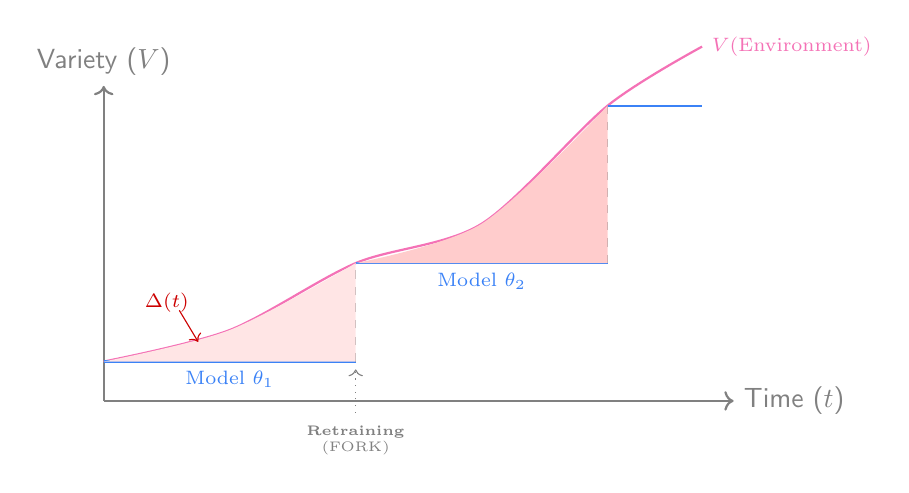
\begin{tikzpicture}[x=0.8cm, y=0.5cm, font=\sffamily]

    % Axes
    \draw[->, thick, gray] (0,0) -- (10,0) node[right] {Time ($t$)};
    \draw[->, thick, gray] (0,0) -- (0,8) node[above] {Variety ($V$)};

    % Real World Complexity (The Disturbance) - Curving up
    \draw[thick, forkcolor, smooth] plot coordinates {(0,1) (2,1.8) (4,3.5) (6,4.5) (8,7.5) (9.5, 9)};
    \node[forkcolor, anchor=west, font=\scriptsize] at (9.5, 9) {$V(\text{Environment})$};

    % AI Model State (The Controller) - Step Function
    \draw[thick, codecolor] (0,1) -- (4,1);
    \draw[dashed, gray] (4,1) -- (4,3.5);
    \draw[thick, codecolor] (4,3.5) -- (8,3.5);
    \draw[dashed, gray] (8,3.5) -- (8,7.5);
    \draw[thick, codecolor] (8,7.5) -- (9.5,7.5);

    % Labels for Model
    \node[codecolor, anchor=north, font=\scriptsize] at (2,1) {Model $\theta_1$};
    \node[codecolor, anchor=north, font=\scriptsize] at (6,3.5) {Model $\theta_2$};

    % The Gap (Error)
    \fill[red!10] (0,1) -- (4,1) -- (4,3.5) -- plot[smooth] coordinates {(4,3.5) (2,1.8) (0,1)} -- cycle;
    \fill[red!20] (4,3.5) -- (8,3.5) -- (8,7.5) -- plot[smooth] coordinates {(8,7.5) (6,4.5) (4,3.5)} -- cycle;

    % Annotations
    \node[anchor=west, text=red!80!black, font=\scriptsize] at (0.5, 2.5) {$\Delta(t)$};
    \draw[->, red!80!black] (1.2, 2.3) -- (1.5, 1.5);

    \node[align=center, font=\tiny, gray] at (4, -1) {\textbf{Retraining}\\(FORK)};
    \draw[->, gray, dotted] (4, -0.3) -- (4, 0.8);

\end{tikzpicture}
\caption{\textbf{The Temporal Variety Gap.} Environmental variety $V(e)$ evolves continuously (curve). A fixed model $\theta$ (stepped line) diverges from reality. The shaded area represents accumulated error. Only \textbf{FORK} rights allow the gap to be closed via retraining.}
\label{fig:variety_gap}
\end{figure}

\subsection{Resource Barriers to Forkability}

The right to \textbf{FORK} a learned system is constrained by physical resources rather than just copyright. In traditional software, the cost to fork is the cost of storage; in AI, the cost to fork is the cost of compute.

\begin{table}[htbp]
\centering
\begin{tabular}{@{}lll@{}}
\toprule
\textbf{Layer} & \textbf{Cost} & \textbf{Barrier} \\
\midrule
Inference code & Minimal & None \\
Running open weights & Low & Minor \\
Fine-tuning & Moderate & Economic \\
Retraining from scratch & Very high & Structural \\
\bottomrule
\end{tabular}
\caption{Resource barriers to forking learned systems}
\end{table}

If a community has the legal right to fork a model but lacks access to the original training data or the massive compute clusters required to reproduce it, the ``Fork'' is illusory.

\begin{claim}
Legal permission to fork without access to compute or data is meaningless. This is an infrastructure question, not a licensing question.
\end{claim}

\subsubsection{The Compute Capture Problem}
\label{subsubsec:compute-capture}

\begin{principle}[Compute Capture]
Training forkability is functionally impossible when the compute cost to retrain a model exceeds the compute accessible to plausible non-operator actors by more than a policy-determined multiplier. Releasing weights while hoarding compute is \textbf{inference forkability without training forkability}.
\end{principle}

If a company releases weights but training cost exceeds 100$\times$ global academic compute capacity, training forkability is zero. The formal determination appears in Appendix~\ref{appendix:proofs}.

\subsubsection{Compute as Governance Infrastructure}

This implies that \textbf{compute is itself DPI}. Legal forkability is insufficient absent practical compute accessibility. Architectural responses include: (1) \textbf{Public Compute Nodes}, state-sponsored clusters with multi-stakeholder governance; (2) \textbf{Mandatory Cost Disclosure}, FLOP estimates and data manifests; (3) \textbf{Federated Training Pools}, distributed training across independent nodes; (4) \textbf{Compute Vouchers}, grants for reproduction attempts.

\subsubsection{Minimum Evidence for Learned System Forkability}
\label{subsubsec:ai-fork-evidence}

To prevent ``FORK fails'' from becoming a rhetorical claim rather than a verifiable determination, learned systems must satisfy specific evidentiary requirements:

\begin{table}[htbp]
\centering
\small
\caption{Evidence requirements for FORK in learned systems}
\label{tab:ai-fork-evidence}
\begin{tabular}{@{}llp{6cm}@{}}
\toprule
\textbf{Artifact} & \textbf{Status} & \textbf{Verification} \\
\midrule
Inference code & Required & Open source license; build reproducibility \\
Model weights & Required & Public download; hash verification \\
Training data manifest & Required & Data Sheets \citep{gebru2021} with provenance \\
Training checkpoint & Recommended & Enables fine-tuning without full retrain \\
Training code & Required & Includes preprocessing, hyperparameters \\
Compute cost estimate & Required & FLOP estimate or cloud cost documentation \\
Successful reproduction & Decisive & Third-party retrain within 10\% of benchmark \\
\bottomrule
\end{tabular}
\end{table}

\paragraph{Forkability Determination.} A learned system passes FORK if:
\begin{enumerate}[noitemsep]
    \item All ``Required'' artifacts are publicly available under permissive terms
    \item The compute cost estimate demonstrates feasibility for at least one non-operator entity (government research consortium, academic cluster, or distributed compute pool)
    \item Either a successful third-party reproduction exists, OR the training code + data manifest enables reproduction in principle
\end{enumerate}

Systems that publish weights but withhold training data or code achieve only \textbf{inference forkability}, not \textbf{training forkability}. Inference forkability permits running the model; training forkability permits correcting it. Only the latter satisfies FORK for governance purposes.

\paragraph{Concrete Examples.} As of 2026, most ``open'' models achieve only inference forkability:
\begin{itemize}[noitemsep]
    \item \textbf{Inference forkability only:} Llama 3 (Meta), DeepSeek, Gemma (Google), Mistral. Weights are published, but training data remains proprietary and full training code is not disclosed. Users can run and fine-tune these models but cannot independently reproduce or audit the training process.
    \item \textbf{Training forkability:} OLMo (Allen Institute), Pythia (EleutherAI). These projects publish weights, complete training code, and full data manifests (Dolma and The Pile respectively). Third parties have successfully reproduced training runs, satisfying the FORK test.
\end{itemize}
The distinction matters: when Llama or Gemma exhibit unexpected behavior, the community can observe symptoms but cannot diagnose root causes in training data. When OLMo exhibits unexpected behavior, researchers can trace the issue to specific training examples. \textbf{Open weights with closed training pipelines is inference transparency without correction capacity.}

\paragraph{Alignment with OSI Definition.} The Open Source Initiative's Open Source AI Definition 1.0 (2024) codifies this distinction, requiring: (1) data information sufficient for recreation, (2) complete training code, and (3) model parameters. By this standard, Llama, Gemma, DeepSeek, and Mistral do not qualify as open source AI despite marketing claims. The framework's FORK test operationalizes the same principle: without training forkability, governance correction is structurally impossible.

\subsection{Agentic Scaling and Governance Denial of Service}
\label{subsec:gdos}

As DPI transitions to support the ``Agentic Economy,'' corrigibility moves from a moral preference to an engineering requirement. Autonomous agents lack the biological resilience to handle bureaucracy.

This framework distinguishes structural corrigibility from ``AI Alignment.'' Alignment asks: \textit{Can the operator control the system?} Corrigibility asks: \textit{Can the affected subject correct the system?} Structural legitimacy requires the latter.

\subsubsection{Corrigibility as an API Contract for Agents}

\begin{itemize}[noitemsep]
    \item \textbf{EXIT is Exception Handling}: To an agent, a mandatory system with no exit path appears as a logic deadlock.
    \item \textbf{CODE is Documentation}: Agents require inspectability of logic to form valid plans.
    \item \textbf{AUDIT is Observability}: An optimization agent cannot function without a reliable failure signal.
    \item \textbf{GOVERN is Constraint Discovery}: Advisory guidelines result in undefined behavior for software agents.
\end{itemize}

\begin{claim}
Incorrigible infrastructure is structurally incompatible with AI automation.
\end{claim}

\subsubsection{The Human Friction Buffer}

Incorrigible infrastructures may appear stable under human load because humans absorb friction through delay, compliance, and informal workaround. Autonomous agents remove this buffering layer.

\paragraph{Illustrative Scenario.} Consider an autonomous procurement agent that interacts with a mandatory payment API. On encountering a compliance flag, the agent receives an opaque error code. No machine-readable error taxonomy exists, and dispute resolution is human-mediated. The agent retries, triggering repeated failures and queue saturation. Human agents absorb such friction via manual override and phone calls; fleets of autonomous agents cannot. The result is a governance denial-of-service (GDoS) that cascades across the payment rail.

As agentic interaction scales, centralized governance mechanisms face \textbf{Governance Denial of Service (GDoS)}: the volume, speed, and strategic diversity of agent actions exceeds the system's capacity to audit, interpret, and correct behavior.

This is not a security failure but a control-theoretic inevitability. Systems lacking distributed audit and rapid, binding governance lack the requisite variety to remain stable under agentic scaling. The correction velocity inequality (Section~\ref{subsec:velocity}) predicts precisely this failure mode: when $\frac{dE}{dt} \gg \frac{dC}{dt}$, the system diverges. Agents accelerate $E(t)$; centralized governance cannot accelerate $C(t)$.

\begin{claim}
Agentic scaling amplifies the correction velocity inequality. Systems that are marginally stable under human interaction rates become catastrophically unstable under agent interaction rates. The human friction buffer is not a feature; it is a hidden subsidy that masks architectural incorrigibility.
\end{claim}

\subsection{Workflow Sovereignty and the Rule of Workflow}
\label{subsec:workflow-sovereignty}

The final mutation of digital infrastructure is the transition from static registries to \textbf{Workflow Orchestration layers} (e.g., Palantir-style data fusion or agentic AI pipelines). In this regime, the operating layer of the state is no longer a ledger of records, but an orchestration of decisions.

\subsubsection{From Rule of Law to Rule of Workflow}

In classical governance, policy is defined in statute, executed by bureaucracy, and reviewed by courts. In a ``Rule of Workflow'' regime, policy becomes emergent from the orchestration logic: data schemas define reality, prompts define interpretation, and API contracts define valid inputs.

\textbf{Workflow Capture} is formalized as follows. Let $W$ be the orchestration layer, $M$ the underlying model, $S$ the state policy function, and $D$ the decision output. While classical governance assumes $S \rightarrow D$, AI-native governance operates as:
\begin{equation}
S \rightarrow W(M, \text{Data}) \rightarrow D
\end{equation}

If $W$ is proprietary and non-forkable, the state's ability to alter policy ($\Delta S$) vanishes because outcomes are constrained by the workflow's technical affordances. Policy debate is reduced to parameter tuning within a vendor-controlled ontology.

\begin{figure}[htbp]
\centering
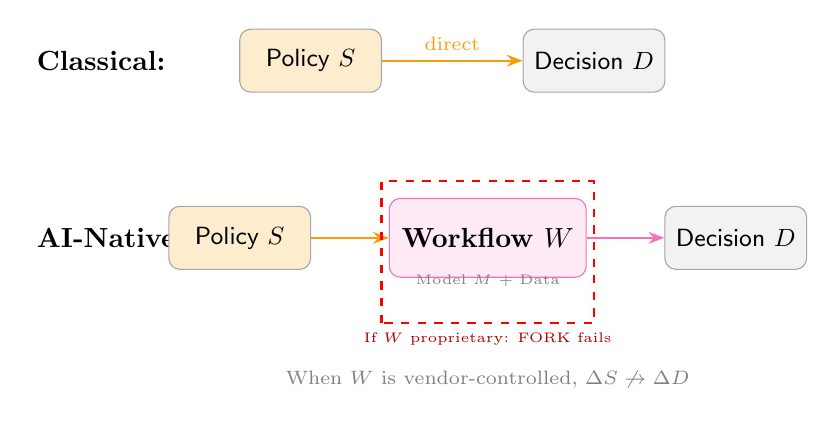
\begin{tikzpicture}[scale=0.9, font=\sffamily\small,
    block/.style={rectangle, rounded corners, draw=gray!70, fill=gray!10, minimum width=1.8cm, minimum height=0.8cm},
    wblock/.style={rectangle, rounded corners, draw=forkcolor, fill=forkcolor!15, minimum width=2.5cm, minimum height=1cm, font=\bfseries},
    arrow/.style={-{Stealth[length=2mm]}, thick}
]

% Classical Governance (top)
\node[anchor=west, font=\bfseries] at (-4, 2.5) {Classical:};
\node[block, fill=governcolor!20] (S1) at (0, 2.5) {Policy $S$};
\node[block] (D1) at (4, 2.5) {Decision $D$};
\draw[arrow, governcolor] (S1) -- (D1) node[midway, above, font=\scriptsize] {direct};

% AI-Native Governance (bottom)
\node[anchor=west, font=\bfseries] at (-4, 0) {AI-Native:};
\node[block, fill=governcolor!20] (S2) at (-1, 0) {Policy $S$};
\node[wblock] (W) at (2.5, 0) {Workflow $W$};
\node[block] (D2) at (6, 0) {Decision $D$};

% Internal to W
\node[font=\tiny, text=gray] at (2.5, -0.6) {Model $M$ + Data};

\draw[arrow, governcolor] (S2) -- (W);
\draw[arrow, forkcolor] (W) -- (D2);

% Capture indicator
\draw[thick, red, dashed] (1, -1.2) rectangle (4, 0.8);
\node[font=\tiny, text=red!70!black, anchor=north] at (2.5, -1.2) {If $W$ proprietary: FORK fails};

% Legend
\node[font=\scriptsize, text=gray, align=left] at (2.5, -2) {When $W$ is vendor-controlled, $\Delta S \not\rightarrow \Delta D$};

\end{tikzpicture}
\caption{\textbf{Workflow Capture.} Classical governance: policy directly determines decisions. AI-native governance: policy is mediated by workflow orchestration. If the workflow is proprietary, policy changes cannot reliably change outcomes.}
\label{fig:workflow-capture}
\end{figure}

\subsubsection{The Workflow Capture Coefficient}

To measure the risk of \textbf{Epistemic Delegation}, the framework proposes the \textbf{Workflow Capture Coefficient (WCC)}: a function of workflow reproduction cost, ontological substitutability, and data/model portability. A high WCC (approaching 1) triggers a failure of the \textbf{FORK} test, regardless of whether the underlying model weights are open. \textbf{Open weights with closed workflows is performative transparency.} The formal operationalization appears in Appendix~\ref{appendix:neutrality}.

\subsubsection{Fallout Governance}

When AI decision throughput outruns human legislative correction velocity, the state enters \textbf{Fallout Governance}: policy ceases to guide behavior in advance; it instead reacts post-hoc to scandal, litigation, or failure clusters. Governance becomes damage containment: the Collingridge Dilemma at civilizational scale.

\subsubsection{Implications for the DPI Trilemma}

The DPI Trilemma is most structurally acute for states operating under external platform dominance and capital-intensive scaling constraints. In such contexts, maximizing Sovereignty and Scale typically requires centralized orchestration, which places structural pressure on execution-layer Neutrality. This is not a policy preference but a control-theoretic constraint: centralization reduces governance variety, and reduced variety erodes the system's capacity to treat diverse inputs equitably under Ashby's Law. The constraint is architectural rather than inevitable and may be mitigated through federated implementation, multi-issuer requirements, and protocol-based rather than platform-based infrastructure design.

\subsection{Architecture-Specific Risk Summary}

The preceding analysis enables architecture-specific risk diagnosis. Different model architectures exhibit distinct failure profiles across the five tests and the new RCR dimension.

\begin{table}[htbp]
\centering
\caption{\textbf{Topology-Aware Corrigibility Risk.} Impact of architectural class on structural tests. Notation: W = weights opacity, G = gating opacity, R = representation opacity, S = scale barrier, O = ontological capture, F = fragmentation, $\kappa$ = compute capture.}
\label{tab:topology-risk-arch}
\small
\begin{tabular}{@{}lllllll@{}}
\toprule
\textbf{Architecture} & \textbf{EXIT} & \textbf{CODE} & \textbf{$\Delta O$ (RCR)} & \textbf{AUDIT} & \textbf{GOVERN} & \textbf{FORK} \\
\midrule
Dense LLM & Partial & Fail (W) & Medium & Partial & Fail (S) & Fail ($\kappa$) \\
Mixture of Experts & Medium & Fail (G) & Medium & Fail (S) & Partial & \textbf{Pass} \\
World Model & Fail (O) & Fail (R) & \textbf{Very Low} & Partial & Partial & Fail ($\kappa$) \\
Edge / SLM & \textbf{Pass} & \textbf{Pass} & High & Fail (F) & Fail (F) & \textbf{Pass} \\
\bottomrule
\end{tabular}
\end{table}

\textbf{Interpretation:} Dense LLMs fail FORK due to compute capture ($\kappa$). World models present the highest RCR (lowest $\Delta O$) because their representation schemas encode administrative ontologies that resist contestation. Edge/SLM models pass EXIT and FORK but may fail GOVERN due to fragmented deployment making coordinated governance infeasible.

\section{Discussion}
\label{sec:discussion}

This section addresses three themes: methodological foundations, political economy, and implementation pathways.

\subsection{Methodological Foundations}
\label{subsec:methodology}

\subsubsection{The Cybernetics of Binary Evaluation}

Critics argue this framework's binary pass/fail topology is too rigid, proposing instead "maturity models" or graded scorecards. From a cybernetic perspective, we reject this gradation. Corrigibility is a \textbf{structural connectivity state}: a feedback loop is either closed or open. There is no ``mostly closed'' loop.

A system that allows \textbf{AUDIT} but blocks \textbf{GOVERN} is an \textbf{Open Loop}: it observes errors but cannot fix them. A system that allows \textbf{GOVERN} but blocks \textbf{EXIT} is a \textbf{Coercive Loop}: it traps energy until catastrophic failure. Partial compliance creates ``zombie infrastructure'': systems maintaining the aesthetic of responsiveness while severing actual stability capacity. A ``Partial'' score represents \textbf{Fatal Structural Failure}.

For diagnostic purposes, gradation remains useful. Tables~\ref{tab:operational-proxies-main} and~\ref{tab:three-indicator-main} specify continuous measurements. The binary determination is the output; continuous measurements are inputs. Evaluators can examine inputs to prioritize interventions.

\subsubsection{Legitimacy Threshold vs Physical Claim}

A critical clarification: the binary model is a \textbf{legitimacy threshold}, not a physical claim about feedback dynamics. Control theorists correctly observe that real systems exhibit continuous variation in loop gain, observability, and actuation authority. A sensor with 50\% accuracy transmits \textit{some} signal; partial actuation produces \textit{some} correction.

The framework does not dispute this physical reality. It makes a normative claim: \textbf{below a threshold of feedback quality, a system forfeits the right to claim public legitimacy}. The threshold is binary because legitimacy is binary. A prison that permits appeals 10\% of the time is still a prison.

\paragraph{Sensitivity Analysis.} Let continuous inputs be $\{p, v, \tau, b, r\}$ (penalty ratio, visibility, latency, bindingness, resource ratio) as defined in Table~\ref{tab:operational-proxies-main}. The binary determination function $D$ is:

\begin{equation}
D = \mathbf{1}[p \leq p^*] \land \mathbf{1}[v \geq v^*] \land \mathbf{1}[\tau \leq \tau^*] \land \mathbf{1}[b = \text{true}] \land \mathbf{1}[r \leq r^*]
\end{equation}

where $\mathbf{1}[\cdot]$ is the indicator function and $\{p^*, v^*, \tau^*, r^*\}$ are threshold values. This formulation makes explicit that:
\begin{enumerate}[noitemsep]
    \item Continuous inputs are preserved for diagnosis
    \item The AND-conjunction enforces the ``weakest link'' principle
    \item Threshold calibration is a policy choice, separable from the structural argument
\end{enumerate}

Systems near thresholds warrant scrutiny; systems far below thresholds across multiple dimensions are unambiguously incorrigible. The binary output serves regulatory clarity; the continuous inputs serve diagnostic priority.

\subsubsection{Continuous Indicators for Diagnostic Use}

The continuous measurements underlying binary determinations enable both threshold calibration and diagnostic prioritization. Table~\ref{tab:operational-proxies-main} specifies operational proxies; Table~\ref{tab:three-indicator-main} formalizes the three-indicator protocol.

\begin{table}[htbp]
\centering
\caption{Operational proxies for the five tests. Thresholds are illustrative and subject to calibration.}
\label{tab:operational-proxies-main}
\begin{tabular}{lll}
\toprule
\textbf{Test} & \textbf{Proxy Metric} & \textbf{Illustrative Threshold} \\
\midrule
EXIT & Penalty ratio $p$ & $p \leq 1.2$ \\
CODE & Visibility fraction $v$ & $v \geq 0.9$ \\
AUDIT & Mean time to detect (MTTD) & MTTD $\leq$ 24 hours \\
GOVERN & Bindingness + throughput $\tau$ & binding = true, $\tau \geq 1$ per 10k users/day \\
FORK & Resource feasibility ratio $r$ & $r \leq 10^{-3}$ \\
\bottomrule
\end{tabular}
\end{table}

\textbf{Interpretation:} Penalty ratio $p$ = cost(non-digital alternative) / cost(digital). Visibility $v$ = public LOC / total LOC on critical execution path. Resource ratio $r$ = estimated FLOP to retrain / aggregate community compute capacity.

\begin{table}[htbp]
\centering
\scriptsize
\caption{Three-indicator protocol: continuous score, binary flag, and threshold metric for each test.}
\label{tab:three-indicator-main}
\begin{tabular}{@{}lp{2.8cm}p{2.8cm}p{3.2cm}@{}}
\toprule
\textbf{Test} & \textbf{Continuous} & \textbf{Binary} & \textbf{Threshold} \\
\midrule
EXIT & \texttt{penalty\_ratio}: exit cost / stay cost & \texttt{legal\_barrier}: criminalized? & $p \leq 1.2$ AND barrier = false \\
CODE & \texttt{visibility}: public LOC / critical path LOC & \texttt{build\_repro}: deterministic build? & $v \geq 0.95$ AND build = true \\
AUDIT & \texttt{observability}: \% verifiable transactions & \texttt{access}: third parties test? & $o \geq 0.9$ AND access = true \\
GOVERN & \texttt{override\_rate}: operator overrule rate & \texttt{charter}: irrevocable instrument? & $r = 0$ AND charter = true \\
FORK & \texttt{cost\_ratio}: fork / community resources & \texttt{rights}: permissive license? & $c \leq 0.001$ AND rights = true \\
\bottomrule
\end{tabular}
\end{table}

\paragraph{Inter-Rater Calibration.} Before deployment, independent auditors should assess 3--5 systems using this protocol and compare determinations. Disagreements identify threshold calibration issues. Target: $\kappa \geq 0.8$ (Cohen's kappa) for binary determinations.

\paragraph{Policy Constants Summary.} The framework employs several calibration constants that represent policy choices separable from the structural argument. Table~\ref{tab:policy-constants} consolidates these for reference.

\begin{table}[htbp]
\centering
\small
\caption{Policy constants used throughout the framework. Values are recommended defaults; jurisdictions may calibrate based on local conditions.}
\label{tab:policy-constants}
\begin{tabular}{@{}llll@{}}
\toprule
\textbf{Symbol} & \textbf{Name} & \textbf{Range} & \textbf{Section} \\
\midrule
$\theta_E$ & FEE sufficiency threshold & $0.8$--$1.0$ & \ref{subsubsec:fee} \\
$\theta$ & Neutrality stability threshold & $(0, 1]$ & \ref{appendix:neutrality} \\
$\kappa$ & Compute accessibility multiplier & $1$--$2$ & \ref{subsubsec:compute-capture} \\
$\alpha^*$ & Fork adoption critical mass & $0.3$--$0.5$ & \ref{appendix:proofs} \\
$\epsilon$ & Correction friction cost & Context-dependent & \ref{appendix:proofs} \\
WCC & Workflow capture threshold & $> 0.7$ triggers FORK fail & \ref{subsec:workflow-sovereignty} \\
\bottomrule
\end{tabular}
\end{table}

\begin{figure}[htbp]
\centering
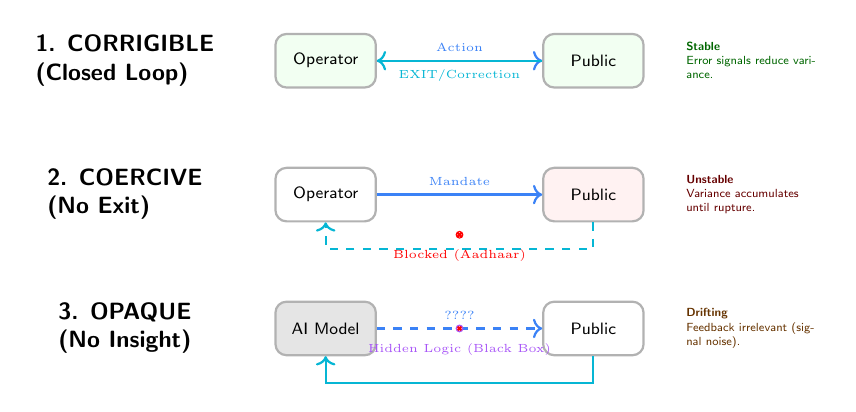
\begin{tikzpicture}[
    scale=0.85, transform shape,
    box/.style={rectangle, draw=gray!60, thick, fill=white, rounded corners, minimum height=0.8cm, minimum width=1.5cm, font=\scriptsize\sffamily},
    lbl/.style={font=\tiny\sffamily\bfseries, color=gray},
    cross/.style={path picture={
        \draw[red, thick] (path picture bounding box.south west) -- (path picture bounding box.north east);
        \draw[red, thick] (path picture bounding box.south east) -- (path picture bounding box.north west);
    }}
]

% -- ROW 1: CORRIGIBLE (Closed Loop) --
\node[font=\bfseries\sffamily, align=left] at (-3, 0) {1. CORRIGIBLE\\(Closed Loop)};
\node[box, fill=green!5] (op1) at (0,0) {Operator};
\node[box, fill=green!5] (us1) at (4,0) {Public};

\draw[->, thick, codecolor] (op1) -- node[above, font=\tiny] {Action} (us1);
\draw[->, thick, exitcolor] (us1) -- node[below, font=\tiny] {EXIT/Correction} (op1);

\node[right=0.5cm of us1, font=\tiny\sffamily, text width=2cm, align=left, color=green!40!black] {
    \textbf{Stable}\\
    Error signals reduce variance.
};

% -- ROW 2: COERCIVE (No Exit) --
\node[font=\bfseries\sffamily, align=left] at (-3, -2) {2. COERCIVE\\(No Exit)};
\node[box] (op2) at (0,-2) {Operator};
\node[box, fill=red!5] (us2) at (4,-2) {Public};

\draw[->, thick, codecolor] (op2) -- node[above, font=\tiny] {Mandate} (us2);
\draw[->, thick, exitcolor, dashed] (us2.south) -- +(0,-0.4) -| (op2.south);
\node[circle, fill=white, draw=red, inner sep=1pt, cross] at (2, -2.6) {};
\node[below, font=\tiny, color=red] at (2, -2.7) {Blocked (Aadhaar)};

\node[right=0.5cm of us2, font=\tiny\sffamily, text width=2cm, align=left, color=red!40!black] {
    \textbf{Unstable}\\
    Variance accumulates until rupture.
};

% -- ROW 3: OPAQUE (No Inspection) --
\node[font=\bfseries\sffamily, align=left] at (-3, -4) {3. OPAQUE\\(No Insight)};
\node[box, fill=gray!20] (op3) at (0,-4) {AI Model};
\node[box] (us3) at (4,-4) {Public};

\draw[->, thick, codecolor, dashed] (op3) -- node[above, font=\tiny] {????} (us3);
\node[circle, fill=white, draw=auditcolor, inner sep=1pt, cross] at (2, -4) {};
\node[below, font=\tiny, color=auditcolor] at (2, -4.1) {Hidden Logic (Black Box)};

\draw[->, thick, exitcolor] (us3.south) -- +(0,-0.4) -| (op3.south);

\node[right=0.5cm of us3, font=\tiny\sffamily, text width=2cm, align=left, color=orange!40!black] {
    \textbf{Drifting}\\
    Feedback irrelevant (signal noise).
};

\end{tikzpicture}
\caption{\textbf{Topologies of Failure.}
(1) A corrigible system closes the loop, converting error signals into stability.
(2) A coercive system blocks \textbf{EXIT}, trapping energy.
(3) An opaque system obscures the action channel, making feedback unintelligible.}
\label{fig:failure_modes}
\end{figure}

\subsection{Corrigibility Under Adversarial Conditions}
\label{subsec:adversarial}

A frequent objection to structural transparency requirements (EXIT, CODE, AUDIT, GOVERN, FORK) concerns adversarial security environments. Critics argue that permitting external audit or interoperability in critical digital infrastructure (particularly identity, payments, or routing rails) may expand the attack surface available to hostile states or organized cyber actors.

This framework does not equate corrigibility with unrestricted public exposure of live exploit vectors. Corrigibility requires \textbf{structured contestability}, not indiscriminate disclosure. The distinction is architectural:

\begin{itemize}[noitemsep]
    \item \textbf{Auditability} refers to verifiable oversight mechanisms (cryptographic proofs, independent inspection rights, reproducible builds, sandboxed red-teaming, hardware-isolated verification environments), not public release of zero-day vulnerabilities.
    \item \textbf{CODE transparency} requires inspectability of system logic and ontology, but does not mandate real-time publication of operational secrets (e.g., private keys, network topologies, live intrusion telemetry).
    \item \textbf{GOVERN mechanisms} may incorporate tiered access controls and certified verifiers, provided the certification process itself remains contestable.
\end{itemize}

Security and corrigibility are not mutually exclusive variables; rather, both depend on layered design. In adversarial contexts, excessive opacity can itself become a systemic vulnerability by preventing early detection of latent design flaws. Historical failures in both public and private infrastructure demonstrate that closed architectures do not eliminate breach risk; they merely concentrate it.

Accordingly, the framework assumes:
\begin{enumerate}[noitemsep]
    \item Security controls may limit raw exploit exposure.
    \item Such controls must not eliminate independent verification pathways.
    \item Emergency override or classified layers must themselves be subject to post-hoc audit.
\end{enumerate}

Corrigibility in adversarial environments therefore implies \textbf{structured verifiability}, not universal visibility. The objective is to preserve corrective bandwidth without compromising defensive posture.

\subsection{Political Economy of Accountability}
\label{subsec:political-economy-discussion}

\subsubsection{The Protocol Model of State}

A common practical objection holds that governments cannot adopt corrigible infrastructure because they must retain control over sovereign functions. This objection relies on a category error: it conflates the \textit{Platform Model} with the \textit{Protocol Model}.

In the \textbf{Platform Model} (currently dominant), the state contracts a vendor to build a monolithic silo (e.g., existing digital ID systems). The vendor controls execution, the state attempts to control policy, and citizens are reduced to rows in a database. As \citet{cohen2019} argues, this model inevitably subverts the Rule of Law by replacing legal due process with optimized platform logic. In the \textbf{Protocol Model} (the corrigible alternative), the state adopts open, corrigible protocols and acts as a high-authority participant within them. The state issues credentials and verifies claims, but it does not enclose the infrastructure itself.

This distinction mirrors the architecture of the web. Governments do not need to build their own proprietary browsers to deliver services; they build sites on HTTP. Similarly, corrigible DPI implies that the state becomes an issuer of trust rather than a landlord of infrastructure. This model does not reduce state capacity; it enhances trust by making the state's operations verifiable.

\subsubsection{Distributed Assessment Capacity}
A corollary objection concerns resources: "Who audits?" The framework does not require every citizen to audit source code. It requires that the infrastructure allows \textit{anyone} to audit, thereby enabling civil society, journalists, and specialized firms to perform this function on behalf of the public. Assessment capacity is itself infrastructure. When systems are designed to be inscrutable, this immune system of society withers.

\subsection{Corrigibility in Extremis}

Incorrigibility is often justified by the rhetoric of necessity, such as national security, anti-corruption, or emergency efficiency. This framework explicitly denies such exemptions. Corrigibility does not imply that substantive rules are negotiable; a system may enforce strict, non-negotiable limits (e.g., pandemic travel restrictions or environmental caps). However, the \textit{structural capacity} to detect error, verify correct enforcement, and reverse wrongful harm must remain intact even in high-constraint environments. As safety engineering demonstrates, accidents in complex systems are caused precisely by the lack of appropriate constraints on component interactions \citep{leveson2011}.

\begin{claim}
No exemption from the five tests is granted on the basis of emergency conditions, planetary constraints, or decentralized architecture.
\end{claim}

This applies equally to decentralized systems. Cryptographic immutability is not a substitute for governance. A blockchain that permanently records a theft without a mechanism for consensus-based reversion is not ``trustless''; it is strictly incorrigible. If a system allows for irrevocable harm without recourse, its decentralization is merely a distribution of unaccountability.

\subsubsection{Political vs Structural Corrigibility}
\label{subsec:political-structural}

A critical objection holds that the framework applies market logic (exit/fork) to non-market systems. You cannot fork India.

The response requires distinguishing two modes of correction:

\begin{itemize}
    \item \textbf{Political corrigibility} (voice via elections): how \textit{states} are corrected
    \item \textbf{Structural corrigibility} (exit/fork): how \textit{infrastructure} is corrected
\end{itemize}

States are corrected politically. DPI sits \textit{below} politics; that is the structural crisis. When DPI is captured by executive authority or vendor monopolies, political correction mechanisms do not reach it. \textbf{Aadhaar operated for seven years under executive fiat before receiving parliamentary authorization as a money bill (2009--2016)} \citep{abraham2016, bhatia2019}.

This is not a hypothetical concern. It is the documented history of the system most frequently cited as a DPI success story. The gap the framework identifies is infrastructure that escapes democratic correction entirely.

Shifting to the \textbf{Protocol Model of State}, where the government acts as an issuer of trust on an open standard rather than a landlord of a private platform, does not surrender sovereignty to technocrats. It returns sovereignty to the legislature, because open protocols cannot be unilaterally weaponized by the executive branch. The Constitution can be amended through democratic process; Aadhaar's architecture cannot be voted on.

\subsubsection{The Distributional Question}
\label{subsec:distributional}

The debate is not ``scale vs sovereignty.'' The debate is \textbf{whose suffering counts}.

\begin{itemize}
    \item Platform speed benefits the median user.
    \item Incorrigibility harms the marginal user.
    \item The marginal user has no voice because EXIT is blocked.
\end{itemize}

Corrigibility is a \textbf{distributional question}. The framework makes visible who bears the cost of system failures. When we ask ``Is this system corrigible?'' we are really asking: ``When this system fails someone, can they do anything about it?''

The answer for Aadhaar is no. Documented starvation deaths in Jharkhand were not caused by ``too much democracy''; they were caused by a system where the marginal user had no recourse when biometric authentication failed.

\subsection{Pathways and Limits}
\label{subsec:pathways}

\subsubsection{Transition Paths}
\label{subsec:transition}

The framework diagnoses incorrigibility but does not prescribe political remedies. However, the structure of the five tests implies an ordering for transition: certain tests are prerequisites for others, and certain interventions have higher leverage.

\subsubsection{Ordered Priorities}

The tests form a dependency chain when considered as a transition sequence:

\begin{enumerate}
    \item \textbf{EXIT first.} Restore exit before other tests. Without exit, no other reform creates genuine feedback. This requires either eliminating mandatory linkage laws or guaranteeing functional non-digital alternatives. EXIT is the error signal; without it, the system cannot sense its own failures.

    \item \textbf{CODE before AUDIT.} Transparency must precede verification. Independent testing is meaningful only if the testing target is observable. Publishing audit results for a black box proves nothing about the box.

    \item \textbf{AUDIT before GOVERN.} Verified error data creates political pressure for governance reform. Governance without measurement is arbitrary. There is no basis for determining whether constraints are adequate. The sensor must function before the actuator can be calibrated.

    \item \textbf{GOVERN enables FORK.} Structural governance can mandate open licensing, data portability, and interoperability requirements that enable eventual forkability. GOVERN without FORK leaves the system captive to its current steward; FORK without GOVERN may produce fragmentation without accountability.
\end{enumerate}

This sequence reflects the causal structure of the feedback loop: signal, sensing, transmission, actuation, selection. Interventions at later stages are ineffective if earlier stages are broken.

\subsubsection{Phase Transitions}

The transition is not gradual improvement. It is a series of phase transitions. Each test either passes or fails; the system remains incorrigible until all five pass. A system that achieves CODE but not EXIT has become transparent without becoming accountable. Users can observe the system's logic but cannot modify their participation.

This explains why open-washing is effective: partial progress creates the appearance of reform while preserving structural capture. The framework rejects partial credit precisely because partial feedback loops do not partially function.

\subsubsection{Political Economy}

The political economy of transition varies by test:

\begin{table}[h]
\centering
\caption{Political economy of transition by test}
\label{tab:political-economy}
\begin{tabular}{lll}
\hline
\textbf{Test} & \textbf{Transition Barrier} & \textbf{Concentrated Opposition} \\
\hline
EXIT & Mandatory linkage laws & Operators lose captive users \\
CODE & Intellectual property claims & Vendors lose competitive moats \\
AUDIT & Security-through-obscurity claims & Operators lose narrative control \\
GOVERN & Sovereignty objections & Executives lose discretion \\
FORK & Typically least opposed & Requires only licensing and documentation \\
\hline
\end{tabular}
\end{table}

FORK is typically the least opposed transition because it requires only legal permission and technical documentation. It does not immediately threaten operator control. However, FORK without the prior four tests is meaningless: the right to reproduce a system you cannot inspect, verify, govern, or exit provides no actual power.

\subsubsection{Cost Considerations}

Transition is not costless. The European Commission \citep{eu2021oss} estimated that public sector open-source adoption yields cost-benefit ratios above 1:4, but this ratio assumes successful implementation. Transition costs include personnel retraining, system compatibility engineering, procurement policy updates, and organizational change.

However, these costs must be weighed against the costs of continued incorrigibility:

\begin{itemize}
    \item Litigation costs from unresolvable grievances
    \item Political instability from suppressed correction demand (Section~\ref{subsec:velocity})
    \item Technical debt from opacity-enabled shortcuts
    \item Vendor lock-in premiums from non-forkable dependencies
    \item Human costs: documented deaths, exclusions, and deprivations
\end{itemize}

The systems in Table~\ref{tab:positive} demonstrate that corrigibility at scale is economically sustainable. Linux, Kubernetes, and Let's Encrypt operate at population scale with resource models that have proven durable over decades.

\subsubsection{Coordination Goods and Inherent Unforkability}
\label{subsec:coordination}

The forking paradox presents a genuine limitation: if you can fork the Public Infrastructure, it may no longer be public.

A ``public'' good (like law or money) derives its value from universality. We all agree on the same truth. If the Identity System is ``forkable,'' and I fork it to create ``Blue-Identity'' while you use ``Red-Identity,'' we have destroyed the common knowledge required for society to function.

\begin{remark}[Latent Forkability in Coordination Goods]
Identity, money, and law are coordination goods; their value derives from uniqueness. If the exercise of FORK destroys the society's ability to coordinate, it functions as mutually assured destruction.

The framework resolves this through \textbf{Latent Forkability}. The stable equilibrium is latent forkability combined with strong coordination incentives. Email coordinates globally not because everyone forks SMTP daily, but because the \textit{credible threat} of doing so prevents any single operator from enclosing the system. \textbf{Latent forkability disciplines the center.} The framework penalizes \textit{constructed legal barriers} to reproduction, not the \textit{natural economic friction} of network effects.
\end{remark}

Whether this equilibrium is achievable for identity infrastructure remains an open question, but the existence of federated identity systems (X-Road, Matrix, AT Protocol) demonstrates that latent forkability is technically achievable even for coordination-sensitive infrastructure.

\subsubsection{Engaging ``Regulate the Loop''}
\label{subsec:regulate}

A sophisticated objection accepts the diagnosis but rejects the prescription:

\begin{quote}
``We accept your Diagnosis (The Loop is Broken). We reject your Prescription (Break the Platform). We choose to \textbf{Regulate the Loop} rather than Fork the Code, because the cost of Forking is Poverty.''
\end{quote}

This argument has force. UPI moved from 0 to over 20 billion monthly transactions in 8 years \citep{npci2026}. Email standardization took decades. India does not have decades. Poverty is now.

\textbf{Where this lands:}
\begin{itemize}
    \item RBI \textit{could} mandate error rate disclosure, demographic audits, grievance SLOs
    \item Political correction (parliament, courts) exists even without FORK
    \item Speed-to-scale tradeoff is real
\end{itemize}

\textbf{Where this misses:}
\begin{itemize}
    \item ``Regulate the loop'' assumes trustworthy regulators. RBI reports to Finance Ministry. UIDAI is executive authority with no parliamentary oversight. Who regulates the regulator?
    \item In captured states, ``regulate later'' means ``never''
    \item Gmail $\neq$ UPI: Gmail \textit{earned} users with features: you CAN leave for Proton, Fastmail, self-hosted. UPI has \textit{regulatory monopoly}: you CANNOT build a competing instant payment switch. Gmail is incorrigible by choice. UPI is incorrigible by law.
    \item ``Regulate later'' rarely happens: Aadhaar 2009 pilot $\rightarrow$ 2016 mandatory $\rightarrow$ 2018 Supreme Court $\rightarrow$ still no real audit. 15 years. Where's the regulation?
\end{itemize}

This tension is not hypothetical. A documented debate between advocates of open standards (arguing for specification transparency and independent security audits) and proponents of centralized control (arguing that controlled governance enables ``faster iteration'') reveals the core disagreement \citep{abraham2020}. The efficiency argument is genuine; but efficiency without accountability is capture dressed as service.

\subsection{Utility Does Not Equal Accountability}
\label{subsec:utility}

A system can be \textbf{useful AND structurally captured}. Both are true simultaneously.

UPI \textit{has} democratized payments. The framework risks dismissing real-world impact if this is not acknowledged. But the question the framework asks is different: \textbf{When UPI fails someone, can they correct it?}

The answer is no. This is the point.

The framework measures \textbf{accountability structure}, not \textbf{utility}. A system can score 0/5 and still be beneficial. The score indicates \textit{structural risk}, not \textit{current harm}. A house built without fire exits can function perfectly for decades, until there is a fire.

\subsection{Institutional Preconditions for Large-Scale Corrigibility}
\label{subsec:institutional}

The framework presumes the existence of intermediary institutions capable of exercising audit, representation, and governance functions. At population scales involving tens or hundreds of millions, spontaneous civic coordination cannot be assumed.

Unlike open-source software communities, where contributors are self-selected and technically specialized, state-scale infrastructure must serve heterogeneous populations with asymmetric digital literacy, resource access, and organizational capacity. The structural availability of audit rights does not guarantee their effective exercise.

Accordingly, structural corrigibility requires:

\begin{description}[noitemsep]
    \item[Independent Verification Bodies] Publicly funded or legally mandated audit institutions insulated from operator control.
    \item[Civic Technical Intermediaries] NGOs, academic labs, and watchdog entities with standing to invoke GOVERN mechanisms.
    \item[Distributed Representation Channels] Mechanisms allowing affected groups to escalate systematic errors collectively, rather than solely through individual grievance.
    \item[Anti-Capture Safeguards] Rotation requirements, transparency obligations for auditors, and conflict-of-interest constraints to prevent elite capture of oversight functions.
\end{description}

The framework does not assume idealized commons governance. It asserts instead that without institutionalized intermediaries, formal corrigibility tests degrade into symbolic compliance.

In this sense, \textbf{corrigibility is necessary but not sufficient for equitable outcomes}. Institutional capacity determines whether structural safeguards translate into practical accountability.

\section{Conclusion and Transition Paths}

Digital Public Infrastructure is not a specific technology; it is a claim of political legitimacy. It asserts that a system is sufficiently foundational, accessible, and accountable to serve as the substrate of civic life.

This paper argues that such legitimacy cannot be derived from self-declarations, "open standards" labeling, or multilateral endorsements. It relies on a specific cybernetic property: \textbf{Corrigibility}. The capacity of the governed to observe the rules, verify their execution, limit their reach, and, if necessary, reproduce the infrastructure to escape its capture.

This paper has proposed five rigorous tests to verify this capacity. The analysis demonstrates that systems currently touted as DPI models (Aadhaar, UPI, and proprietary AI) fail these tests, revealing them to be administrative enclosures rather than public goods. Conversely, the systems which actually run the world (Linux, Kubernetes, the Web) pass them structurally.

\subsection{The Asymmetry of Intelligence}

The problem of AI-DPI governance is not a problem of intelligence, but a problem of \textbf{infrastructural asymmetry}. Corrigibility declines not because models are powerful, but because centralized scaling concentrates compute, ontology, and routing control into fewer hands. The five tests diagnose this concentration; they do not measure capability.

A world model running on distributed edge devices with open weights, published representation schemas, and federated governance would pass all five tests regardless of its intelligence. A narrow classifier running on centralized infrastructure with opaque logic and mandatory participation would fail regardless of its simplicity. The framework is architecture-sensitive, not capability-sensitive.

This reframing matters for policy. The discourse of ``AI risk'' often conflates capability with capture. Corrigibility separates these concerns: a system can be simultaneously powerful and accountable, or weak and authoritarian. The question is not ``How smart is it?'' but ``Can those it affects correct it?'' As Section~\ref{subsec:institutional} establishes, corrigibility requires institutional capacity to translate structural safeguards into practical accountability.

\subsection{The Roadmap Out}

The structure of the five tests implies an ordering for transition (detailed in Section~\ref{subsec:pathways}): EXIT $\to$ CODE $\to$ AUDIT $\to$ GOVERN $\to$ FORK. This sequence reflects the causal structure of the feedback loop. Interventions at later stages are ineffective if earlier stages are broken.

\subsection{The Core Finding}

The choice is not between chaos and control. It is between \textbf{Open Loop} systems that drift toward fragility and authoritarianism, and \textbf{Closed Loop} systems that stabilize themselves through the correction of those they serve.

\begin{quote}
\textit{Systems that cannot be corrected by those they affect will eventually be corrected by forces they cannot control.}
\end{quote}

\subsection{Summary of Topological Risk}

The ``physics'' of digital governance demonstrates that certain architectures structurally increase the risk of capture independent of operator intent. The transition to AI-native states does not eliminate the need for the Rule of Law; it necessitates its translation into the \textbf{Rule of the Workflow}.

\begin{table}[htbp]
\centering
\caption{Topological risk summary across infrastructure layers}
\label{tab:topological-risk}
\begin{tabular}{llll}
\toprule
\textbf{Layer} & \textbf{Primary Failure Mode} & \textbf{Capture Type} & \textbf{Structural Remedy} \\
\midrule
Ledger & Dependency & Administrative & FEE / Portability \\
Model & Stochasticity & Stochastic & Deterministic Guardrails \\
Ontology & Incontestability & Epistemic & LWD-R Disclosure \\
Workflow & Lock-In & Interpretive & Workflow Forkability (WCC) \\
\bottomrule
\end{tabular}
\end{table}

Corrigibility is the structural response to the Collingridge Dilemma (Section~\ref{subsec:velocity}): architectural constraints must be established before entrenchment makes correction impossible.

\subsection{Limitations}

\begin{enumerate}
    \item \textbf{Binary classification serves legitimacy thresholds, not diagnostic prioritization.} The binary determination answers ``Does this system merit the claim of public infrastructure?'' It does not answer ``Which constraint should reformers address first?'' For diagnostic prioritization, the continuous metrics in Tables~\ref{tab:operational-proxies-main} and~\ref{tab:three-indicator-main} are more useful. A system scoring 4/5 has better structural properties than one scoring 0/5, even though both fail the legitimacy threshold.

    \item \textbf{FORK may be structurally unachievable for essential state infrastructure.} Even with open code, essential state infrastructure faces barriers that technical openness cannot overcome: legal monopoly (the state grants one system validity), network effects (a fork accepted by no one is worthless), data non-portability (identity records do not come with the code), and trust bootstrapping (institutional trust takes decades). The framework provides no demonstrated example of essential state identity infrastructure disciplined by fork threat. For such systems, the framework's value is diagnostic (identifying structural capture) rather than prescriptive (enabling actual forking). Latent forkability may create pressure, but this remains undemonstrated.

    \item \textbf{Functional Exit Equivalence (FEE) is unvalidated.} FEE is proposed as the resolution for the essentiality-corrigibility tension, but no essential identity infrastructure has implemented full FEE. Partial analogues exist (telecom number portability, PSD2 banking APIs), but these operate in domains with weaker network effects than identity. Whether FEE can provide accountability equivalent to true forkability for identity infrastructure remains an open empirical question.

    \item \textbf{The control theory formalization is illustrative, not predictive.} The mapping of GOVERN to $K(s)$ and AUDIT to $H(s)$ illustrates structural relationships; it does not claim that DPI literally behaves as a linear time-invariant system. The insight (broken feedback degrades accountability) is valid as structural analogy. The mathematical formalism should be understood as pedagogical model, not physical prediction. Incorrigible systems may be stable indefinitely; the framework evaluates legitimacy, not stability.

    \item \textbf{The framework is primarily diagnostic, not prescriptive.} This paper provides rigorous criteria for evaluating infrastructure accountability. It does not provide validated prescriptions for building corrigible essential services. The proposed solutions (FEE, open licensing, multi-stakeholder governance) are theoretical constructs requiring empirical validation. The contribution is diagnosis of a possibly fundamental tension, not its resolution.

    \item \textbf{Governance evaluation is judgment-dependent.} GOVERN requires historical evidence of enforcement, making it more interpretation-dependent than technical tests.

    \item \textbf{Resource forkability for AI remains unresolved.} Legal rights without compute access may be permanently unfulfillable for frontier AI systems. The LWD-R requirements (Logic, Weights, Data, Representation) may be impossible for models trained on proprietary, legally encumbered, or practically enormous datasets. The AI extension identifies structural challenges; validated solutions do not yet exist.

    \item \textbf{Timescale argument applies to external remedies.} The critique targets external bureaucracies (courts, ombudsmen), not all deliberative processes. Bitcoin's BIP process operates on human timescales and remains valid governance.

    \item \textbf{Network effects are not formally modeled.} Network effects can make formally forkable systems practically unforkable (e.g., Signal's open code but unfederated network).

    \item \textbf{Empirical analysis centers on India.} The primary case studies (Aadhaar, UPI) derive from India Stack. While the theoretical framework generalizes, systematic validation across other national DPI implementations (Brazil Pix, Singapore NDI, Kenya M-Pesa) is required before universal claims are established.

    \item \textbf{Political economy is not analyzed.} The paper diagnoses structural failures but does not explain why governments choose incorrigible designs when corrigible alternatives exist. Understanding these incentives (efficiency gains, control preferences, vendor capture, path dependence) is essential for policy reform and remains outside this paper's scope.

    \item \textbf{The framework encodes specific values.} This framework prioritizes structural accountability through exit mechanisms (the capacity to leave or reproduce) over voice mechanisms (political participation, democratic oversight). This reflects a specific intellectual tradition (Hirschman's exit/voice distinction, Stallman's free software principles, commons governance theory). Alternative frameworks prioritizing voice have independent value. The framework is not ideologically neutral; it makes explicit what it values.

    \item \textbf{Baseline mortality comparison is not established.} Deaths from Aadhaar-related exclusion are documented. Comparison to pre-Aadhaar baseline mortality from PDS dysfunction (leakage, corruption, exclusion) is not provided in this paper. The structural argument concerns accountability mechanisms (paper systems permitted human override; biometric systems do not), not comparative death rates.
\end{enumerate}

\subsection{Future Work}

Extensions warranting investigation: (1) \textbf{Empirical velocity measurement}, quantifying when systems become ungovernable; (2) \textbf{International comparison}, testing generality across X-Road, Singapore NDI, EU Digital Identity, Brazil Pix; (3) \textbf{Political economy of architecture choice}, examining why governments choose incorrigible designs when corrigible alternatives exist; (4) \textbf{Transition cost modeling}; (5) \textbf{AI verification protocols}, standardized disclosure formats; (6) \textbf{Legal doctrine integration}, operationalizing corrigibility for courts; (7) \textbf{Network effect formalization}; (8) \textbf{Agentic system API contracts}.

\section*{Acknowledgments}

This framework was developed through analysis of India Stack and subsequent generalization to universal criteria. The author thanks the digital rights community for ongoing critique and refinement.

\section*{License}

This work is released under CC0 1.0 Universal (Public Domain). Use, adapt, translate, and redistribute freely. No attribution required.

\section*{Data and Code Availability}

The complete framework, including JSON Schemas for machine-readable disclosure and assessment, is available at:

\begin{itemize}
    \item Framework documentation: \url{https://indiastack.in/dpi/}
    \item Infrastructure manifest schema: \url{https://indiastack.in/dpi/schema/infrastructure.json}
    \item Corrigibility assessment schema: \url{https://indiastack.in/dpi/schema/corrigibility.json}
    \item Paper source and repository: \url{https://github.com/AnivarAravind/corrigibility-framework}
\end{itemize}

% ============================================
% APPENDICES
% ============================================
\appendix

\section{Architecture of Accountability}
\label{appendix:architecture}

To move beyond qualitative debate, this framework establishes a formal logic for accountability. The machine-readable artifacts described below serve not merely as data formats, but as a \textit{digital constitutional binding} that separates operator claims from auditor verification. By enforcing specific data structures, we convert policy rhetoric into falsifiable assertions of system state.

\subsection{Logic: The Adversarial Manifests}

The architecture relies on a separation of concerns mirroring the adversarial legal process. It employs two distinct document types (see Figure~\ref{fig:manifests}):

\begin{enumerate}
    \item \textbf{infrastructure.json (The Operator's Affidavit):} A signed declaration by the system operator asserting specific operational properties, governance commitments, and functional limitations.
    \item \textbf{corrigibility.json (The Auditor's Finding):} An independent, cryptographically signed evaluation that tests the operator's claims against observable reality.
\end{enumerate}

This architecture makes contradictions machine-readable. If an operator claims a governance mechanism is "binding" in their affidavit, but the auditor's observation marks the \texttt{user\_authority} field as "advisory," the mismatch serves as mathematically verifiable proof of governance failure.

\begin{figure}[htbp]
\centering
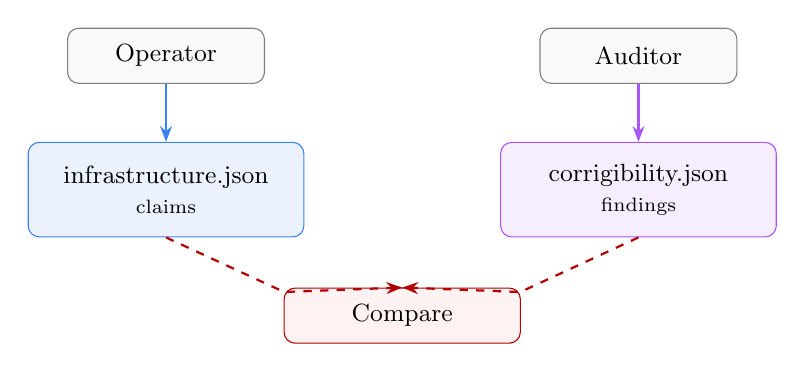
\begin{tikzpicture}[
    manifest/.style={rectangle, rounded corners, draw=#1, fill=#1!10, minimum width=3.5cm, minimum height=1.2cm, font=\small, align=center},
    actor/.style={rectangle, rounded corners, draw=gray, fill=gray!5, minimum width=2.5cm, minimum height=0.7cm, font=\small},
    arrow/.style={-{Stealth[length=2mm]}, thick},
    compare/.style={rectangle, rounded corners, draw=red!70!black, fill=red!5, minimum width=3cm, minimum height=0.7cm, font=\small}
]
\node[actor] (operator) at (0,2.5) {Operator};
\node[actor] (auditor) at (6,2.5) {Auditor};
\node[manifest=codecolor] (infra) at (0,0.8) {infrastructure.json\\{\scriptsize claims}};
\node[manifest=auditcolor] (corrig) at (6,0.8) {corrigibility.json\\{\scriptsize findings}};
\draw[arrow, codecolor] (operator) -- (infra);
\draw[arrow, auditcolor] (auditor) -- (corrig);
\node[compare] (compare) at (3,-0.8) {Compare};
\draw[arrow, red!70!black, dashed] (infra.south) -- (1.5,-0.5) -- (compare.north);
\draw[arrow, red!70!black, dashed] (corrig.south) -- (4.5,-0.5) -- (compare.north);
\end{tikzpicture}
\caption{Adversarial Verification Architecture. Operators declare; Auditors verify. The structural gap constitutes the audit finding.}
\label{fig:manifests}
\end{figure}

\subsection{Interpretation: The Non-Authoritativeness of Determination}

A critical logic gate in this framework is the derivation of status.

\begin{claim}
The \texttt{determination} object in \texttt{corrigibility.json} is a derived convenience field. It is \textbf{not authoritative}.
\end{claim}

Any value asserted in \texttt{determination} MUST be mechanically recomputed from the \texttt{tests} object by evaluators or courts. If an auditor asserts \texttt{corrigible: true} but the \texttt{tests} object contains a failure, the manifest is strictly invalid. This rule ensures that no actor (operator, auditor, or regulator) can "declare" a system corrigible by fiat; status exists only as the computed sum of observable structural properties.

\section{Formal Structural Model}
\label{appendix:proofs}

\paragraph{Executive Summary (Non-Technical Overview).}
This appendix formalizes two core claims of the paper using control theory as a structural model:
\begin{enumerate}[noitemsep]
    \item \textbf{Null-Feedback Instability:} If any component of the feedback path is structurally severed, the system operates as open-loop and will diverge under persistent disturbance.
    \item \textbf{Correction Velocity Inequality:} If the rate of digital error propagation exceeds the rate of institutional correction, post-hoc remedies are insufficient to prevent systemic failure.
\end{enumerate}
This formalization illustrates structural relationships between the five tests and feedback system properties. It does not claim that DPI literally behaves as a linear time-invariant system; the model is pedagogical, clarifying why partial compliance represents structural failure rather than partial success.

\medskip

To formalize the assertion that ``partial corrigibility is a fatal structural failure,'' we model Digital Public Infrastructure as a standard feedback control system subject to environmental disturbance.

\subsection{Open-Loop Instability Model}

Let a DPI system state $y(t)$ (actual impact) be expected to track a reference target $r(t)$ (intended policy/rights), subject to environmental disturbance $d(t)$ (attacks, changing demographics, fraud).

The error signal (grievance) is defined as:
\begin{equation}
e(t) = r(t) - y(t)
\end{equation}

In a closed-loop system, the corrective action $u(t)$ (GOVERN) is a function of the detected error via a feedback controller $K$ (GOVERN logic) and a sensor transfer function $H$ (AUDIT/EXIT mechanism):
\begin{equation}
u(t) = K(t) \cdot H(e(t))
\end{equation}

The plant dynamics (DPI operation) are given by:
\begin{equation}
\dot{y}(t) = u(t) + d(t)
\end{equation}

\begin{theorem}[Null-Feedback Instability]
If any component of the feedback path is structurally broken, specifically if Sensor Transparency $H=0$ (Failed AUDIT) or Actuator Coupling $K=0$ (Failed GOVERN), the system effectively operates as Open Loop. Under Open Loop conditions with non-zero integrating disturbance $d(t)$, the error $e(t)$ diverges unboundedly.
\end{theorem}

\begin{proof}
If tests \textbf{AUDIT} or \textbf{EXIT} fail, $H=0$.
If test \textbf{GOVERN} fails, $K=0$.
In either case, the effective corrective feedback is $u_{fb} = 0$.
The system evolution depends only on initial intent $u_{open}$ and disturbance:
\begin{equation}
y(t) = \int_0^t (u_{open}(\tau) + d(\tau)) d\tau
\end{equation}
Given that environmental variety $d(t)$ is stochastic and non-zero (Ashby's Law), and without negative feedback to compensate:
\begin{equation}
\lim_{t \to \infty} |r(t) - y(t)| \to \infty
\end{equation}
Thus, stability is impossible without the closure of the feedback loop. ``Partial'' corrigibility (where $K=0$ or $H=0$) yields the same asymptotic stability profile as total authoritarianism.
\end{proof}

\begin{corollary}
Corrigibility is a binary structural property. If any one of the five tests (EXIT, CODE, AUDIT, GOVERN, FORK) fails, the system is incorrigible.
\end{corollary}

\textit{Justification}: Each test corresponds to a necessary component of the feedback loop. Partial compliance does not preserve loop closure. This follows directly from Theorem~1: since $L(s) = K(s) \cdot P(s) \cdot H(s)$, if any multiplicative term is zero, the entire loop gain vanishes.

\begin{figure}[htbp]
\centering
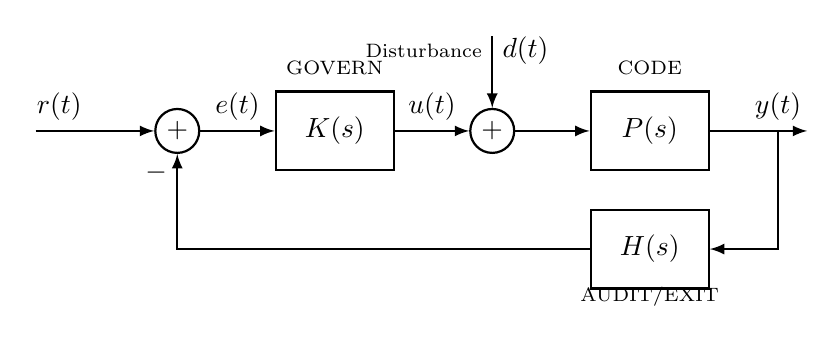
\begin{tikzpicture}[node distance=1.8cm, auto, >=latex, thick]
    % Styles
    \tikzstyle{block} = [draw, rectangle, minimum height=1cm, minimum width=1.5cm]
    \tikzstyle{sum} = [draw, circle, inner sep=2pt]
    \tikzstyle{input} = [coordinate]
    \tikzstyle{output} = [coordinate]

    % Nodes
    \node [input] (rinput) {};
    \node [sum, right of=rinput] (sum1) {$+$};
    \node [block, right of=sum1, node distance=2cm] (K) {$K(s)$};
    \node [sum, right of=K, node distance=2cm] (sum2) {$+$};
    \node [block, right of=sum2, node distance=2cm] (P) {$P(s)$};
    \node [output, right of=P, node distance=2cm] (output) {};
    \node [block, below of=P, node distance=1.5cm] (H) {$H(s)$};
    \node [input, above of=sum2, node distance=1.2cm] (disturbance) {};

    % Labels
    \node [above of=K, node distance=0.8cm] {\scriptsize GOVERN};
    \node [below of=H, node distance=0.6cm] {\scriptsize AUDIT/EXIT};
    \node [above of=P, node distance=0.8cm] {\scriptsize CODE};

    % Connections
    \draw [->] (rinput) -- node[pos=0.2] {$r(t)$} (sum1);
    \draw [->] (sum1) -- node {$e(t)$} (K);
    \draw [->] (K) -- node {$u(t)$} (sum2);
    \draw [->] (sum2) -- (P);
    \draw [->] (P) -- node [name=y, pos=0.7] {$y(t)$} (output);
    \draw [->] (y) |- (H);
    \draw [->] (H) -| node[pos=0.9, left] {$-$} (sum1);
    \draw [->] (disturbance) -- node[pos=0.2, right] {$d(t)$} node[pos=0.2, left] {\scriptsize Disturbance} (sum2);
\end{tikzpicture}
\caption{\textbf{Control-theoretic model of corrigible infrastructure.} $K(s)$: governance controller. $H(s)$: sensor/audit function. $P(s)$: plant (infrastructure). $d(t)$: environmental disturbance.}
\label{fig:control-model}
\end{figure}

The closed-loop transfer function from reference to output is:
\begin{equation}
\frac{Y(s)}{R(s)} = \frac{K(s)P(s)}{1 + K(s)P(s)H(s)}
\end{equation}

The transfer function from disturbance to output is:
\begin{equation}
\frac{Y(s)}{D(s)} = \frac{P(s)}{1 + K(s)P(s)H(s)}
\end{equation}

Corrigibility requires that each component exists and is non-degenerate:
\begin{itemize}
    \item EXIT $\Rightarrow$ $e(t) \neq 0$ observable (error signal exists)
    \item AUDIT $\Rightarrow$ $H(s) \neq 0$ (sensor functional)
    \item GOVERN $\Rightarrow$ $K(s) \neq 0$ (actuator functional)
    \item CODE $\Rightarrow$ $P(s)$ is intelligible
    \item FORK $\Rightarrow$ $P, K, H$ replaceable if convergence fails
\end{itemize}

\noindent \textbf{Active Deception as Sensor Attack.} The pathologies defined in Section~\ref{subsec:active-deception} (open-washing, safety-washing, audit theatre) fundamentally corrupt the sensor function $H(s)$: they either suppress the true error signal $e(t)$ or inject artificial stability metrics, thereby blinding the controller $K(s)$ to the actual divergence $y(t) - r(t)$. In control-theoretic terms, Active Deception renders $H(s) \to 0$ not by removing the sensor, but by making its output uncorrelated with the true system state.

\begin{figure}[htbp]
\centering
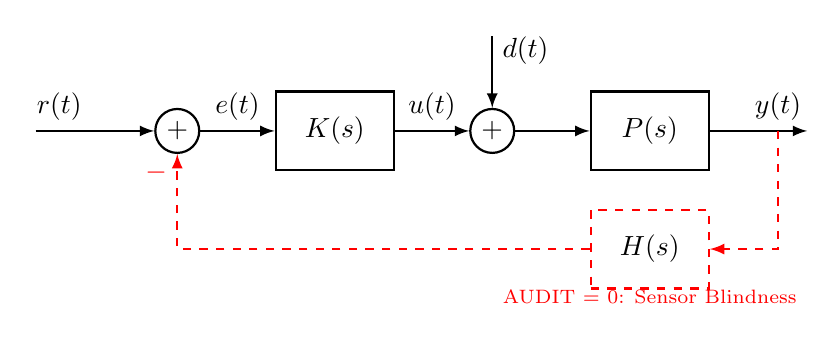
\begin{tikzpicture}[node distance=1.8cm, auto, >=latex, thick]
    \tikzstyle{block} = [draw, rectangle, minimum height=1cm, minimum width=1.5cm]
    \tikzstyle{sum} = [draw, circle, inner sep=2pt]
    \tikzstyle{input} = [coordinate]
    \tikzstyle{output} = [coordinate]

    \node [input] (rinput) {};
    \node [sum, right of=rinput] (sum1) {$+$};
    \node [block, right of=sum1, node distance=2cm] (K) {$K(s)$};
    \node [sum, right of=K, node distance=2cm] (sum2) {$+$};
    \node [block, right of=sum2, node distance=2cm] (P) {$P(s)$};
    \node [output, right of=P, node distance=2cm] (output) {};
    \node [block, below of=P, node distance=1.5cm, draw=red, dashed] (H) {$H(s)$};
    \node [input, above of=sum2, node distance=1.2cm] (disturbance) {};

    \node [below of=H, node distance=0.6cm, red] {\scriptsize AUDIT = 0: Sensor Blindness};

    \draw [->] (rinput) -- node[pos=0.2] {$r(t)$} (sum1);
    \draw [->] (sum1) -- node {$e(t)$} (K);
    \draw [->] (K) -- node {$u(t)$} (sum2);
    \draw [->] (sum2) -- (P);
    \draw [->] (P) -- node [name=y, pos=0.7] {$y(t)$} (output);
    \draw [->, dashed, red] (y) |- (H);
    \draw [->, dashed, red] (H) -| node[pos=0.9, left] {$-$} (sum1);
    \draw [->] (disturbance) -- node[pos=0.2, right] {$d(t)$} (sum2);
\end{tikzpicture}
\caption{\textbf{Open-loop failure mode.} When AUDIT fails ($H = 0$), the feedback path is severed. Equivalent failure occurs if GOVERN ($K = 0$) or EXIT ($e(t) \equiv 0$) is removed.}
\label{fig:open-loop}
\end{figure}

\subsection{The Strict Correction Velocity Inequality}

For the system to remain stable not just asymptotically but locally (preventing irreversible harm), the correction rate must dominate the error rate. We formalize this with a friction coefficient.

\begin{condition}[Strict Dynamic Stability]
\label{cond:friction}
Let $\epsilon > 0$ represent the ``friction cost'' of correction (e.g., litigation time, protest cost). A system is stable iff:
\begin{equation}
\left| \frac{d}{dt} C(t) \right| \ge \left| \frac{d}{dt} E(t) \right| + \epsilon
\end{equation}
\end{condition}

\textbf{Implication:} Post-hoc remedies (Courts/Ombudsmen) have a linear or constant rate of operation ($\frac{dC}{dt} = k$). Digital errors propagate at exponential or high-frequency rates ($\frac{dE}{dt} \propto e^{t}$). Since there is no $t$ for which a linear function dominates an exponential one, relying on external courts guarantees eventual system collapse. The correction logic must be intrinsic to the loop.

\begin{figure}[htbp]
\centering
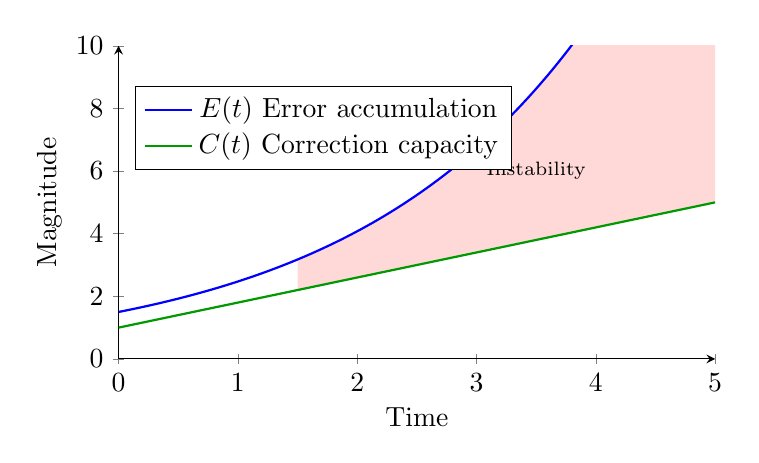
\begin{tikzpicture}[scale=0.9]
    \begin{axis}[
        xlabel={Time},
        ylabel={Magnitude},
        xmin=0, xmax=5,
        ymin=0, ymax=10,
        legend pos=north west,
        axis lines=left,
        domain=0:5,
        samples=100,
        width=10cm,
        height=6cm
    ]
    \addplot[blue, thick, name path=E] {1.5*exp(0.5*x)};
    \addlegendentry{$E(t)$ Error accumulation}
    \addplot[green!60!black, thick, name path=C] {1 + 0.8*x};
    \addlegendentry{$C(t)$ Correction capacity}
    \addplot[red!30, opacity=0.5] fill between[of=E and C, soft clip={domain=1.5:5}];
    \node at (axis cs:3.5,6) {\scriptsize Instability};
    \end{axis}
\end{tikzpicture}
\caption{\textbf{Correction velocity mismatch.} Error $E(t)$ accumulates faster than correction $C(t)$ in bureaucratic systems. The shaded region represents accumulated unresolved harm.}
\label{fig:velocity-mismatch}
\end{figure}

\subsection{Mapping to the Five Tests}

\begin{table}[htbp]
\centering
\caption{Mapping corrigibility tests to control-theoretic components}
\label{tab:control-mapping}
\begin{tabular}{lll}
\hline
\textbf{Test} & \textbf{Control Component} & \textbf{Failure Mode} \\
\hline
EXIT & Error Signal & Reference collapse \\
CODE & Signal Integrity & Noise indistinguishable from intent \\
AUDIT & Sensor & Blind control \\
GOVERN & Actuator & No corrective force \\
FORK & Variety Expansion & Monolithic collapse \\
\hline
\end{tabular}
\end{table}

\subsection{Agentic Interoperability Requirements}

For an autonomous agent $\mathcal{A}$ to operate reliably within infrastructure $\mathcal{I}$, the following predicates must be strictly True:

\begin{enumerate}
    \item \textbf{Reversibility:} $\forall$ state $s_t \in \mathcal{S}$, $\exists$ transition $s_{t+1}$ (via \texttt{EXIT}) such that $\text{Cost}(s_{t+1}) < \infty$. (No deadlocks).
    \item \textbf{Decidability:} $\forall$ input $x$, $\text{Compute}(x) \to \{0,1\}$ is inspectable via \textbf{CODE}. (No hidden constraints).
\end{enumerate}

Failure of these predicates renders $\mathcal{I}$ a ``Hazmat Environment'' for automated agents, effectively blocking the agentic economy.

\begin{figure}[htbp]
\centering
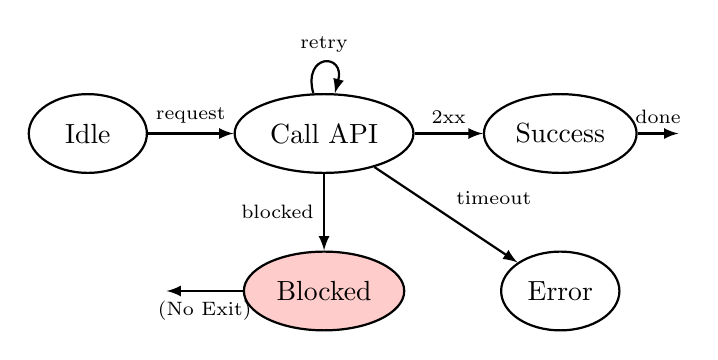
\begin{tikzpicture}[node distance=2cm, auto, >=latex, thick]
    \tikzstyle{state} = [draw, ellipse, minimum width=1.5cm, minimum height=1cm]
    \tikzstyle{blocked} = [draw, ellipse, minimum width=1.5cm, minimum height=1cm, fill=red!20]

    \node [state] (idle) {Idle};
    \node [state, right of=idle, node distance=3cm] (call) {Call API};
    \node [state, right of=call, node distance=3cm] (success) {Success};
    \node [blocked, below of=call, node distance=2cm] (blocked) {Blocked};
    \node [state, below of=success, node distance=2cm] (error) {Error};

    \draw [->] (idle) -- node {\scriptsize request} (call);
    \draw [->] (call) -- node {\scriptsize 2xx} (success);
    \draw [->] (success) -- node {\scriptsize done} ++(1.5,0);
    \draw [->] (call) -- node[left] {\scriptsize blocked} (blocked);
    \draw [->] (call) to[loop above, looseness=5] node {\scriptsize retry} (call);
    \draw [->] (call) -- node {\scriptsize timeout} (error);
    \draw [->] (blocked) -- node[below] {\scriptsize (No Exit)} ++(-2,0);
\end{tikzpicture}
\caption{\textbf{Agentic automaton.} Without EXIT and observable error codes, agent loops indefinitely, times out, or escalates incorrectly.}
\label{fig:agentic-automaton}
\end{figure}

\subsection{Measurement Procedures for Reproducibility}
\label{subsec:measurement}

To enable third-party reproduction of pass/fail determinations, each test requires specific evidence types:

\begin{table}[htbp]
\centering
\small
\caption{Evidence requirements for reproducible assessment}
\label{tab:evidence-requirements}
\begin{tabular}{@{}lp{5cm}p{5cm}@{}}
\toprule
\textbf{Test} & \textbf{Required Evidence} & \textbf{Verification Method} \\
\midrule
EXIT & (1) Legal mandate status, (2) documented alternative pathways, (3) penalty documentation & Survey of legal instruments; cost comparison with alternatives; user testimony \\
CODE & (1) Source repository URL, (2) build reproducibility proof, (3) execution path coverage & Hash verification; deterministic build; static analysis of critical paths \\
AUDIT & (1) API documentation, (2) data access agreement, (3) historical error rate publication & Attempt independent measurement; verify data freshness; compare operator vs independent findings \\
GOVERN & (1) Charter/statute URL with hash, (2) governance action log, (3) enforcement history & Legal analysis; search for overruled operator decisions; verify binding mechanism \\
FORK & (1) License text, (2) technical artifact availability, (3) resource cost estimate, (4) successful fork examples & License audit; attempt reproduction; cost modeling; historical fork survey \\
\bottomrule
\end{tabular}
\end{table}

\paragraph{Reproducibility Standard.} An assessment is reproducible if an independent auditor, given only the evidence artifacts listed above, reaches the same pass/fail determination. Disagreements must trace to (a) threshold calibration differences or (b) missing evidence, not to ambiguity in the test definitions themselves. Continuous metrics and threshold protocols are provided in Tables~\ref{tab:operational-proxies-main} and~\ref{tab:three-indicator-main} (Section~\ref{subsec:methodology}).

\subsection{Network Adoption Model for Fork Feasibility}

Model adoption fraction $\alpha(t)$. A community-spawned fork succeeds if $\alpha$ crosses critical mass $\alpha^*$. Logistic adoption with social influence:
\begin{equation}
\dot{\alpha} = \beta \alpha(1 - \alpha) + s(t)
\end{equation}
where $s(t)$ is exogenous seeding. Fork feasibility requires parameters such that $\exists t$ with $\alpha(t) \geq \alpha^*$. Practical condition:
\begin{equation}
s_{\min} \geq \alpha^* - \alpha_0
\end{equation}
or subsidies that accelerate adoption rate $\beta$.

\begin{figure}[htbp]
\centering
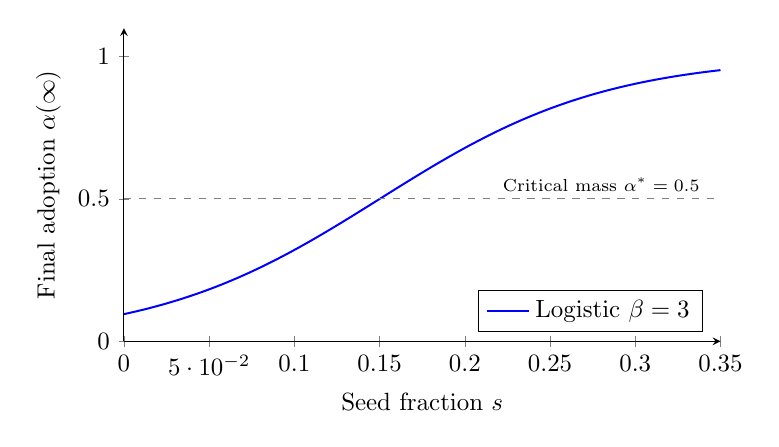
\begin{tikzpicture}[scale=0.9]
    \begin{axis}[
        xlabel={Seed fraction $s$},
        ylabel={Final adoption $\alpha(\infty)$},
        xmin=0, xmax=0.35,
        ymin=0, ymax=1.1,
        legend pos=south east,
        axis lines=left,
        width=10cm,
        height=6cm
    ]
    \addplot[blue, thick, domain=0:0.35, samples=100] {1/(1+exp(-15*(x-0.15)))};
    \addlegendentry{Logistic $\beta = 3$}
    \draw[dashed, gray] (axis cs:0,0.5) -- (axis cs:0.35,0.5);
    \node at (axis cs:0.28,0.55) {\scriptsize Critical mass $\alpha^* = 0.5$};
    \end{axis}
\end{tikzpicture}
\caption{\textbf{Fork feasibility curve.} Below critical seeding, adoption does not reach critical mass. Parameters illustrative.}
\label{fig:fork-feasibility}
\end{figure}

\subsection{Extended Formal Models}

\subsubsection{Linearized Sensitivity Model}

For small perturbations around a nominal operating point, the sensitivity function characterizes how disturbances propagate to the output:
\begin{equation}
S(s) = \frac{1}{1 + L(s)}
\end{equation}
where $L(s) = K(s) \cdot P(s) \cdot H(s)$ is the loop gain. When any corrigibility test fails ($K=0$, $H=0$, or error signal blocked), $L(s) \to 0$ and $S(s) \to 1$: disturbances pass through unattenuated.

\subsubsection{Discrete Integrator Example}

Consider a discrete-time scalar integrator modeling cumulative harm:
\begin{equation}
y_{k+1} = y_k + d_k - u_k
\end{equation}
where $d_k$ is the disturbance (errors, attacks) and $u_k$ is the correction. In open loop ($u_k = 0$):
\begin{equation}
y_N = y_0 + \sum_{k=0}^{N-1} d_k
\end{equation}

For any non-zero mean disturbance $\mathbb{E}[d_k] = \mu > 0$, the expected state grows linearly: $\mathbb{E}[y_N] = y_0 + N\mu \to \infty$. This provides a simple, indisputable demonstration of open-loop divergence.

\textbf{Friction cost in discrete model:} The friction coefficient $\epsilon$ from Condition~\ref{cond:friction} manifests in this discrete model as a delay or reduction in the correction term. Specifically, if correction requires bureaucratic processing with latency $\tau$ time steps and efficiency loss $\eta < 1$, then:
\begin{equation}
u_k = \eta \cdot f(y_{k-\tau}, d_{k-\tau})
\end{equation}
where $f(\cdot)$ is the feedback policy. When $\tau > 0$ or $\eta < 1$, the effective correction rate is reduced, directly corresponding to the continuous-time friction cost $\epsilon > 0$. The stability condition $|dC/dt| \geq |dE/dt| + \epsilon$ translates to requiring the feedback policy to over-correct relative to the disturbance rate, accounting for these frictional losses.

\subsubsection{Formal Error and Correction Rates}

Let $E(t)$ denote cumulative error (total harm or divergence from policy) and $C(t)$ denote cumulative correction applied. Define:
\begin{itemize}
    \item \textbf{Error generation rate:} $\dot{E}(t) = \frac{dE}{dt}$
    \item \textbf{Effective correction rate:} $\dot{C}(t) = \frac{dC}{dt}$
\end{itemize}

The system is stable only if the net error remains bounded:
\begin{equation}
E(t) - C(t) < M \quad \forall t > 0
\end{equation}

This requires $\dot{C}(t) \geq \dot{E}(t)$ on average. When correction operates through bureaucratic channels with bounded throughput $\dot{C}_{\max}$ while errors grow exponentially, there exists a critical time $t^*$ beyond which correction can never catch up.

\subsection{Compute Capture Formalization}

Let $C_{\text{train}}$ be the compute cost required to retrain a model, and $C_{\text{accessible}}$ be the compute accessible to plausible non-operator actors (academic clusters, government research consortiums, distributed compute pools). Training forkability is functionally impossible when:
\begin{equation}
C_{\text{train}} > \kappa \cdot C_{\text{accessible}}
\label{eq:compute-capture}
\end{equation}
where $\kappa$ is an accessibility multiplier (policy constant, typically $1 \leq \kappa \leq 2$).

The formal determination becomes:
\begin{equation}
\text{FORK}_{\text{training}} = \mathbf{1}[C_{\text{train}} \leq \kappa \cdot C_{\text{accessible}}] \land \mathbf{1}[\text{data\_manifest\_available}]
\label{eq:fork-training}
\end{equation}

where $\mathbf{1}[\cdot]$ is the indicator function and \texttt{data\_manifest\_available} requires Data Sheets for Datasets with full provenance.

\subsection{Functional Exit Equivalence Formalization}

An essential system $S$ satisfies FEE if compensatory architectural guarantees recreate the same effective error-signal strength that exit provides in non-essential systems.

Let:
\begin{itemize}[noitemsep]
    \item $E_{\text{exit}}^{\text{baseline}}$ = effective error-signal strength produced by real exit (non-essential case)
    \item $E_{\text{alt}}(S)$ = effective error-signal strength produced by compensatory mechanisms (essential case)
\end{itemize}

\begin{equation}
\text{FEE}(S) \iff E_{\text{alt}}(S) \geq \theta_E \cdot E_{\text{exit}}^{\text{baseline}}
\label{eq:fee}
\end{equation}

where $\theta_E$ is a policy calibration constant (recommended range: $0.8$--$1.0$).

\paragraph{Operationalizing $E$.} The error-signal strength $E$ can be operationalized as a weighted sum:

\begin{equation}
E = \alpha_1 \cdot \text{effective\_loss} + \alpha_2 \cdot \text{probability\_of\_departure} + \alpha_3 \cdot \text{velocity\_of\_response} + \alpha_4 \cdot \text{legal\_remedy\_speed}
\label{eq:error-signal}
\end{equation}

where the weights $\alpha_i$ are calibrated via pilot audits. All variables are operationalized such that higher values indicate greater corrective pressure on the operator.

\subsection{Switching Cost Formalization}

The practical barrier to exit and fork is operationalized through a \textbf{switching cost} scalar:

\begin{equation}
\sigma(S \to S') = c_{\text{data}} + c_{\text{downtime}} + c_{\text{reprovisioning}} + c_{\text{network}} + c_{\text{legal}}
\label{eq:switching-cost}
\end{equation}

where each component is normalized to $[0,1]$:
\begin{itemize}[noitemsep]
    \item $c_{\text{data}}$: cost of exporting and reformatting user data
    \item $c_{\text{downtime}}$: service interruption during transition
    \item $c_{\text{reprovisioning}}$: re-establishing credentials and trust relationships
    \item $c_{\text{network}}$: loss of social connections and network effects
    \item $c_{\text{legal}}$: regulatory friction and contractual barriers
\end{itemize}

\paragraph{Portability Threshold.} EXIT and FORK functionally fail when switching cost to all plausible alternatives exceeds a policy threshold:

\begin{equation}
\min_{S' \in \mathcal{A}} \sigma(S \to S') > \Sigma^* \implies \text{EXIT/FORK fail}
\label{eq:portability-threshold}
\end{equation}

where $\mathcal{A}$ is the set of available alternatives and $\Sigma^*$ is a calibrated threshold (e.g., $>0.2$ of annual disposable income or $>30$ days service disruption).

\paragraph{Illustrative Application.} Aadhaar exhibits $\sigma \approx 4.8$ (near-maximal) because $c_{\text{data}} = 1$ (no export), $c_{\text{downtime}} = 1$ (total service denial), and $c_{\text{legal}} = 1$ (mandate forecloses alternatives). UPI retains $\sigma \approx 1.0$--$1.5$ because cash and cards remain legal. With $\Sigma^* = 2.0$, Aadhaar categorically fails EXIT/FORK while UPI passes conditionally.

\subsection{Summary of Formal Extensions}

\begin{enumerate}
    \item Linearized result ties removal of $H$, $K$, or EXIT to vanishing loop gain $L(s)$, exposing unstable process modes.
    \item Integrator example supplies simple, indisputable divergence demonstration.
    \item Correction velocity formalized via measurable $C(t)$ and $E(t)$.
    \item Network model clarifies why legal forkability may fail in practice and yields policy levers (seeding, subsidies).
    \item Agent automaton demonstrates need for explicit machine-facing EXIT/CODE/AUDIT primitives.
    \item Switching cost formalization operationalizes EXIT/FORK failure thresholds.
\end{enumerate}

\section{Neutrality Compression Under Centralized Enforcement}
\label{appendix:neutrality}

This appendix provides the formal proof supporting Proposition~\ref{prop:trilemma} (Topology-Dependent Tension) and integrates the Workflow Capture Coefficient into the analysis.

\subsection{Definitions}

Let:
\begin{itemize}[noitemsep]
    \item $Sc$ = Scale (population-level integration)
    \item $V_{\text{env}}(Sc)$ = Environmental variety (heterogeneity of governed interactions)
    \item $V_{\text{gov}}(Sc)$ = Governance corrective variety
    \item $\text{WCC} \in [0,1)$ = Workflow Capture Coefficient
    \item $V_{\text{eff}}$ = Effective corrective variety
\end{itemize}

We assume:
\begin{enumerate}[noitemsep]
    \item $V_{\text{env}}(Sc)$ is non-decreasing in $Sc$
    \item Under centralized enforcement, governance growth is institutionally bounded
\end{enumerate}

Formally:
\begin{equation}
V_{\text{gov}}(Sc) = O(Sc^{\alpha}), \quad \alpha < 1
\end{equation}
This states that governance corrective capacity grows sublinearly under centralized topology. No specific functional form (logarithmic, square root, etc.) is required.

\subsection{Workflow Capture Coefficient Formalization}

The Workflow Capture Coefficient measures the risk of epistemic delegation to proprietary orchestration layers:
\begin{equation}
WCC = f(C_{\text{workflow}}, O_{\text{substitutability}}, M_{\text{portability}})
\end{equation}

Where:
\begin{itemize}[noitemsep]
    \item $C_{\text{workflow}}$ = normalized cost of reproducing the orchestration stack (0 = trivial, 1 = infeasible)
    \item $O_{\text{substitutability}}$ = ease of altering the underlying ontological schema (0 = locked, 1 = fully substitutable)
    \item $M_{\text{portability}}$ = data and model portability across implementations (0 = proprietary lock-in, 1 = fully portable)
\end{itemize}

A simple operationalization uses the weighted harmonic mean:
\begin{equation}
WCC = 1 - \frac{3}{\frac{1}{1-C_{\text{workflow}}} + \frac{1}{O_{\text{substitutability}}} + \frac{1}{M_{\text{portability}}}}
\end{equation}

\paragraph{Why Harmonic Mean?} The choice of harmonic mean over arithmetic or geometric mean is deliberate and mirrors the binary logic of corrigibility. The harmonic mean has a critical property: it is dominated by the smallest input. If any single dimension approaches zero (e.g., portability is near-zero while reproduction cost and substitutability are moderate), the harmonic mean collapses, driving WCC toward 1 (high capture). This matches the framework's core insight that a feedback loop fails if \textit{any} component fails. An arithmetic mean would allow high scores in two dimensions to mask complete failure in a third; the harmonic mean prevents this compensation. Formally, for inputs $x_1, x_2, x_3 \in (0,1]$, if $x_1 \to 0$ while $x_2, x_3$ remain finite, then $H(x_1, x_2, x_3) \to 0$ and $WCC \to 1$.

A high WCC (approaching 1) triggers FORK failure regardless of model weight openness.

\paragraph{Worked Example.} Consider two systems:

\textit{Aadhaar authentication workflow:} $C_{\text{workflow}} = 0.95$ (reproduction requires replicating UIDAI's entire biometric infrastructure), $O_{\text{substitutability}} = 0.1$ (biometric templates are proprietary and non-interoperable), $M_{\text{portability}} = 0.05$ (no data export, no credential portability). Computing:
\[
WCC_{\text{Aadhaar}} = 1 - \frac{3}{\frac{1}{0.05} + \frac{1}{0.1} + \frac{1}{0.05}} = 1 - \frac{3}{20 + 10 + 20} = 1 - 0.06 = 0.94
\]

\textit{X-Road federated workflow:} $C_{\text{workflow}} = 0.3$ (open-source, documented), $O_{\text{substitutability}} = 0.8$ (standard protocols), $M_{\text{portability}} = 0.7$ (data exchange formats are open). Computing:
\[
WCC_{\text{X-Road}} = 1 - \frac{3}{\frac{1}{0.7} + \frac{1}{0.8} + \frac{1}{0.7}} = 1 - \frac{3}{1.43 + 1.25 + 1.43} = 1 - 0.73 = 0.27
\]

Aadhaar's $WCC = 0.94$ indicates near-total workflow capture; X-Road's $WCC = 0.27$ indicates low capture risk. This aligns with the qualitative assessment in Table~\ref{tab:govt_infra}.

\subsection{Effective Governance Under Workflow Capture}

Rather than assume a multiplicative structure, we define a general suppression operator:
\begin{equation}
V_{\text{eff}} = \Psi(V_{\text{gov}}, \text{WCC})
\end{equation}
Where:
\begin{itemize}[noitemsep]
    \item $\Psi$ is increasing in $V_{\text{gov}}$
    \item $\Psi$ is decreasing in WCC
    \item $\Psi(V_{\text{gov}}, 0) = V_{\text{gov}}$
    \item $\Psi(V_{\text{gov}}, \text{WCC}) < V_{\text{gov}}$ for $\text{WCC} > 0$
\end{itemize}
This avoids imposing unjustified linearity or proportionality.

\subsection{Neutrality Condition}

Neutrality does not require full dominance of environmental variety. It requires sufficient corrective bandwidth to prevent systematic routing bias.

Define:
\begin{equation}
V_{\text{eff}} \geq \theta \cdot V_{\text{env}}
\end{equation}
Where $\theta \in (0,1]$ is a stability sufficiency constant.

\textbf{Neutrality degradation risk} emerges when:
\begin{equation}
V_{\text{eff}} < \theta \cdot V_{\text{env}}
\end{equation}
This avoids equating neutrality with perfect stability.

\subsection{Proposition (Formal Statement)}

Under centralized enforcement topology and non-zero workflow capture, there exists a scale threshold $Sc^*$ beyond which neutrality is at risk unless governance growth becomes at least linear in scale.

\subsection{Proof}

Assume:
\begin{equation}
V_{\text{env}}(Sc) = \Omega(Sc)
\end{equation}

Under centralized enforcement:
\begin{equation}
V_{\text{gov}}(Sc) = O(Sc^{\alpha}), \quad \alpha < 1
\end{equation}

Since $\Psi$ is monotonic increasing in $V_{\text{gov}}$ and decreasing in WCC, and bounded above by $V_{\text{gov}}$:
\begin{equation}
V_{\text{eff}}(Sc) \leq V_{\text{gov}}(Sc)
\end{equation}

Therefore:
\begin{equation}
\frac{V_{\text{eff}}(Sc)}{V_{\text{env}}(Sc)} \to 0 \quad \text{as} \quad Sc \to \infty
\end{equation}

Thus there exists $Sc^*$ such that:
\begin{equation}
V_{\text{eff}}(Sc^*) < \theta \cdot V_{\text{env}}(Sc^*)
\end{equation}

The neutrality condition is violated. \qed

\subsection{Governance Automation Objection}

One may argue that governance capacity scales linearly through AI monitoring. However:

If governance automation is implemented within the same centralized workflow topology, then:
\begin{itemize}[noitemsep]
    \item WCC increases
    \item Ontology substitutability decreases
    \item External corrective independence does not increase proportionally
\end{itemize}

Thus governance automation does not automatically imply:
\begin{equation}
V_{\text{gov}}(Sc) = \Theta(Sc)
\end{equation}
unless corrective mechanisms are externally independent and substitutable.

This preserves the proposition.

\subsection{Falsifiability Clause}

The theory would be falsified if a centralized sovereign DPI:
\begin{enumerate}[noitemsep]
    \item Achieves population-scale deployment
    \item Maintains governance growth $V_{\text{gov}}(Sc) = \Theta(Sc)$
    \item Exhibits low workflow capture ($\text{WCC} \approx 0$)
    \item Sustains structural neutrality under high scale
\end{enumerate}
\textit{without} federated or multi-operator architecture.

Such a system would contradict the sublinear governance constraint. This condition is empirically testable.

\subsection{Interpretation}

The result does not assert:
\begin{itemize}[noitemsep]
    \item That scale is harmful
    \item That sovereignty is undesirable
    \item That neutrality is impossible
\end{itemize}

It asserts:
\begin{itemize}[noitemsep]
    \item Under centralized enforcement topology, governance corrective capacity must scale at least linearly with environmental complexity to preserve neutrality.
    \item If workflow capture suppresses corrective bandwidth, neutrality degradation risk becomes a structural prediction.
\end{itemize}

\begin{figure}[htbp]
\centering
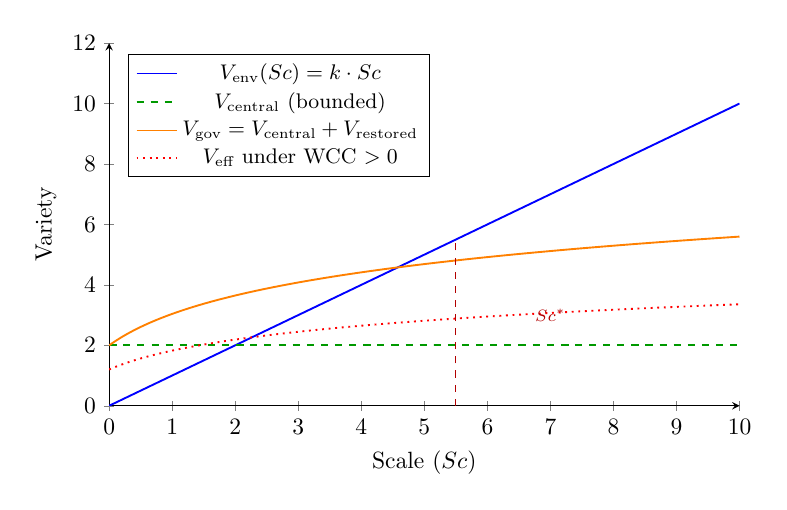
\begin{tikzpicture}[scale=0.85]
    \begin{axis}[
        xlabel={Scale ($Sc$)},
        ylabel={Variety},
        xmin=0, xmax=10,
        ymin=0, ymax=12,
        legend pos=north west,
        axis lines=left,
        domain=0:10,
        samples=100,
        width=11cm,
        height=7cm,
        legend style={font=\small}
    ]
    % Environmental variety (linear)
    \addplot[blue, thick] {x};
    \addlegendentry{$V_{\text{env}}(Sc) = k \cdot Sc$}

    % Centralized governance (constant)
    \addplot[green!60!black, thick, dashed] {2};
    \addlegendentry{$V_{\text{central}}$ (bounded)}

    % Restored variety (logarithmic growth)
    \addplot[orange, thick] {2 + 1.5*ln(x+1)};
    \addlegendentry{$V_{\text{gov}} = V_{\text{central}} + V_{\text{restored}}$}

    % Effective variety under WCC (suppressed)
    \addplot[red, thick, dotted] {0.6*(2 + 1.5*ln(x+1))};
    \addlegendentry{$V_{\text{eff}}$ under WCC $> 0$}

    % Mark critical threshold
    \node[font=\scriptsize, text=red!70!black] at (axis cs:7,3) {$Sc^*$};
    \draw[red!70!black, dashed, thin] (axis cs:5.5,0) -- (axis cs:5.5,5.5);
    \end{axis}
\end{tikzpicture}
\caption{\textbf{Governance Variety Compression Under Scale.} As scale increases, environmental variety grows linearly. Under centralized enforcement, governance variety grows sublinearly. Workflow capture further suppresses effective corrective bandwidth. Neutrality degradation risk emerges when effective governance variety falls below environmental complexity (at $Sc^*$).}
\label{fig:variety-compression}
\end{figure}

\section{Schema Specifications and Automated Assessment}
\label{appendix:schema}

\paragraph{Executive Summary (Machine-Readable Corrigibility).}
This appendix provides illustrative JSON schemas demonstrating how corrigibility tests can be operationalized in machine-readable form. These schemas are not implementation mandates; they are reference architectures showing how error taxonomies, binding governance mechanisms, and audit transparency can be encoded as enforceable technical constraints. The objective is to demonstrate that corrigibility can be implemented as infrastructure logic rather than advisory policy.

\medskip

To move beyond qualitative debate, this framework establishes a machine-readable logic for accountability via two JSON schemas: the \texttt{infrastructure.json} (Operator Disclosure) and the \texttt{corrigibility.json} (Auditor Assessment). By enforcing specific data structures, policy rhetoric is converted into falsifiable assertions of system state.

\subsection{Architecture}

The architecture relies on a separation of concerns mirroring the adversarial legal process:

\begin{enumerate}[noitemsep]
    \item \textbf{infrastructure.json (Operator's Affidavit):} A signed declaration by the system operator asserting specific operational properties, governance commitments, and functional limitations. Key fields include \texttt{offline\_equivalent} (tracking EXIT), \texttt{when\_uncertain} (tracking AI safety failures), and \texttt{layers} (enabling decomposed evaluation).

    \item \textbf{corrigibility.json (Auditor's Finding):} An independent, cryptographically signed evaluation that tests the operator's claims against observable reality. Key fields include \texttt{penalty\_ratio} (quantifying coerciveness), \texttt{visibility} (CODE inspection level), and \texttt{user\_authority} (GOVERN binding status).
\end{enumerate}

This architecture makes contradictions machine-readable. If an operator claims a governance mechanism is ``binding'' in their affidavit, but the auditor's observation marks the \texttt{user\_authority} field as ``advisory,'' the mismatch serves as mathematically verifiable proof of governance failure.

\subsection{Schema Repository}

Due to space constraints, the full normative JSON schemas (v1.7) with exhaustive validation rules are hosted externally. The schemas include:

\begin{itemize}[noitemsep]
    \item Exhaustive field definitions for all five tests
    \item Layer-decomposed evaluation structures
    \item Learned system extensions (model role, uncertainty handling)
    \item Cryptographic signing requirements (Ed25519, DID anchoring)
\end{itemize}

Researchers and auditors may access, validate, and contribute to these schemas via the permanent repository: \url{https://indiastack.in/dpi/schema/}. The framework source code, including validation scripts suitable for CI/CD integration, is available at the GitHub repository listed in the Data and Code Availability section.

\section{Verification and Enforcement}
\label{appendix:rules}

To distinguish valid governance from performative compliance, the framework enforces strict evidentiary rules for Identity and Authority.

\subsection{Normative Rules}

\paragraph{Rule A.9: Operational Definition of Binding Authority}
To satisfy the GOVERN test, any escalation path claimed as "binding" in the Manifest MUST include:
\begin{enumerate*}[label=(\roman*)]
    \item a resolvable reference to the statute or charter (\texttt{binding\_proof\_url}),
    \item a cryptographic hash of that instrument to prevent silent amendment, and
    \item historical evidence of enforcement against the operator.
\end{enumerate*}
Assertions of authority that rely on post-execution bureaucratic discretion (e.g., ombudsmen, "feedback forms") DO NOT satisfy this rule and must be marked \texttt{false}.

\paragraph{Rule A.10: Chain of Custody}
Auditor manifests must be canonically serialized (RFC 8785), hashed (SHA-256), and signed (Ed25519) using a valid W3C Decentralized Identifier. Unsigned assessments are treated as schema-invalid. This creates a permanent, falsifiable record of who certified a system.

\subsection{Identity Assurance Model}

To prevent "Identity Washing", where operators use ephemeral keys to rubber-stamp their own systems, the framework employs a Tiered Assurance Model. Verification dashboards should weigh assessments accordingly:

\begin{enumerate}
    \item \textbf{Tier 1: Self-Attested (\texttt{did:key}):} Ephemeral identity. Suitable for whistleblowers, individual researchers, or rapid-response checks. \textit{Status: Informational.}
    \item \textbf{Tier 2: Domain-Verified (\texttt{did:web}):} Identity cryptographically bound to a specific DNS domain (e.g., \texttt{did:web:eff.org}). Attribution to known civil society actors. \textit{Status: Verified.}
    \item \textbf{Tier 3: Institution-Verified:} Identity anchored in transparency logs or institutional trust registries. \textit{Status: Regulatory Standing.}
\end{enumerate}

\section{Framework Evolution}
\label{appendix:evolution}

This framework did not evolve through theoretical speculation; it hardened through adversarial engagement with live systems. Each version update represents the closure of a specific "loophole" used by operators to claim public legitimacy while retaining private control.

\begin{description}[style=nextline, leftmargin=1em, labelindent=0pt]

\item[\textbf{Version 1.0 (Definition)}]
Established the baseline thesis: Corrigibility is a structural precondition, distinct from feature sets. It defined the five tests to answer the foundational question: \textit{What distinguishes public infrastructure from private monopoly?}

\item[\textbf{Version 1.2 (Assessment)}]
\textbf{Closed the Self-Attestation Loophole.} Early trials showed operators self-declaring success. This version separated the \textit{Infrastructure Manifest} from the \textit{Corrigibility Assessment}, establishing the adversarial verification model where publicness must be proven by independent parties.

\item[\textbf{Version 1.4 (Logic)}]
\textbf{Closed the Ambiguity Loophole.} Eliminated partial credit and "maturity models." The shift to strictly binary logic established that failure in any single dimension breaks the feedback loop required by Ashby's Law, rendering the system unstable.

\item[\textbf{Version 1.5 (Invariance)}]
\textbf{Closed the Exceptionalism Loophole.} Extended the framework to AI and decentralized ledgers, demonstrating that neither statistical opacity nor cryptographic immutability exempts a system from the requirements of Reversibility (EXIT) and Correction (GOVERN).

\item[\textbf{Version 1.6 (Constraint)}]
\textbf{Closed the Consultation Loophole.} Redefined GOVERN as non-overrideable internal constraint rather than advice or redress. Explicitly disqualified post-execution remedies and advisory bodies from constituting system governance.

\item[\textbf{Version 1.6.2 (Reproduction)}]
\textbf{Closed the Substitution Loophole.} Distinguished EXIT (market choice) from FORK (reproduction). Switching landlords is not forking infrastructure.

\item[\textbf{Version 1.7 (Layering)}]
\textbf{Closed the DID-Washing Loophole.} Added layer-decomposed evaluation requiring analysis at each architectural stratum. Systems claiming corrigibility through identifier decentralization while retaining centralized governance at higher layers are now explicitly diagnosed. Introduced the propagation rule: $T_{\text{system}} = \bigwedge T(L_i)$.

\end{description}

\section{Anticipated Objections and Responses}
\label{appendix:objections}

This appendix addresses the strongest objections to the framework, organized by the discipline from which they originate.

\subsection{Control Theory Objections}

\paragraph{Objection 1: Binary model ignores continuous feedback dynamics.}
``Real control systems have continuous loop gain. Partial observability and partial actuation still provide some regulation. Your binary pass/fail ignores systems that are 'mostly corrigible.'''

\textbf{Response:} The objection conflates physical description with normative threshold. We do not dispute that real systems exhibit continuous variation in feedback quality. The binary model is a \textit{legitimacy threshold}, not a physical claim (Section~\ref{sec:discussion}). A feedback loop with 50\% sensor accuracy transmits some signal; this does not mean the system deserves public trust. The determination function $D$ (Section~\ref{subsec:methodology}) makes explicit that continuous inputs feed a binary output. The threshold is where we draw the line for public legitimacy, separable from the physics.

\paragraph{Objection 2: Where is the Lyapunov stability proof?}
``You claim systems diverge without feedback. Show the Lyapunov function. Without rigorous stability analysis, this is hand-waving.''

\textbf{Response:} Appendix~\ref{appendix:proofs} provides the formal treatment. Theorem 1 (Null-Feedback Instability) proves that when $H=0$ or $K=0$, the system operates open-loop and diverges under non-zero disturbance. The discrete integrator example (Section B.6.2) provides an elementary proof: $y_N = y_0 + \sum d_k \to \infty$ for any non-zero mean disturbance. A full Lyapunov treatment would require specifying the state space for a particular DPI implementation; the framework operates at the architectural level, where the key insight (that open loops diverge) is mathematically trivial.

\subsection{Political Science Objections}

\paragraph{Objection 3: You ignore legitimate state interests.}
``Governments have valid reasons for mandatory systems: national security, public health, anti-fraud. Your framework would prohibit pandemic contact tracing.''

\textbf{Response:} The framework does not prohibit mandatory systems; it diagnoses their structural properties. Emergency necessity explains but does not justify incorrigibility (Corollary to Proposition~\ref{prop:essentiality}). A pandemic contact-tracing system can still satisfy CODE (open source), AUDIT (independent testing), GOVERN (binding privacy constraints), and FORK (interoperable protocol). Only EXIT is constrained by mandatory participation. The question is whether the other four tests pass, not whether mandates are ever legitimate. Section~\ref{sec:discussion} explicitly notes that corrigibility is compatible with strict, non-negotiable rules.

\paragraph{Objection 4: Proposition 2 proves your framework is useless.}
``You prove essential services can never be fully corrigible. This makes your framework irrelevant for the systems that matter most: identity, payments, healthcare.''

\textbf{Response:} The proposition identifies a structural constraint, not a reason to abandon analysis. The architectural responses (Section~\ref{subsubsec:arch-responses}) show two paths: protected alternatives (guarantee non-digital equivalents) or federated implementation (no single provider essential). X-Road demonstrates 4/5 at population scale. The finding that fully corrigible essential services require architectural innovation is the framework's central contribution. Diagnosing why current systems fail is prerequisite to designing better ones.

\subsection{Empirical Objections}

\paragraph{Objection 5: Your pass/fail determinations are subjective.}
``Two auditors could reach different conclusions. Without precise, reproducible metrics, this is opinion dressed as science.''

\textbf{Response:} Section~\ref{subsec:measurement} specifies evidence requirements for each test. Table~\ref{tab:evidence-requirements} lists required artifacts and verification methods. The reproducibility standard states: an assessment is reproducible if an independent auditor, given only the evidence artifacts, reaches the same determination. Disagreements must trace to threshold calibration or missing evidence, not definition ambiguity. The JSON schemas (Appendix~\ref{appendix:schema}) enforce structured disclosure. Future work includes inter-rater reliability studies.

\paragraph{Objection 6: FORK is illusory for AI systems.}
``You admit compute costs make AI retraining impractical. If FORK always fails for frontier AI, your framework just says `all AI is incorrigible,' which would be trivially true and useless.''

\textbf{Response:} Section~\ref{subsubsec:ai-fork-evidence} specifies minimum evidence for learned system forkability. The key distinction is \textit{inference forkability} (running weights) vs \textit{training forkability} (reproducing the model). Only training forkability satisfies FORK for governance purposes. The evidence requirements (Table~\ref{tab:ai-fork-evidence}) are achievable: published training code, data manifests, and compute cost estimates. The claim is not that all AI fails FORK, but that systems withholding these artifacts fail. OLMo, Pythia, and academic models demonstrate that FORK-compliant AI is possible; the question is whether frontier labs choose to comply.

\subsection{Summary}

The framework withstands scrutiny from control theory (binary is threshold, not physics), political science (mandates can coexist with corrigibility on other dimensions), and empirical methodology (reproducible metrics exist). The strongest residual objection (network effects making FORK practically impossible even when legally permitted) is acknowledged in Limitations and proposed for formal treatment in Future Work.

\section{Sections Suitable for Standalone Publication}
\label{appendix:opeds}

The following sections from this paper are self-contained and suitable for adaptation as op-eds, policy briefs, or standalone essays:

\begin{description}
\item[Active Deception (Section~\ref{subsec:active-deception})] Defines safety-washing, open-washing, and audit theatre as sensor attacks on accountability infrastructure. Suitable for technology policy audiences.

\item[Climate Washing (Section~\ref{subsubsec:climatewashing})] Analyzes environmental rhetoric in DPI discourse. Suitable for climate and technology policy intersection.

\item[Engaging ``Regulate the Loop'' (Section~\ref{subsec:regulate})] Responds to the ``regulate later'' objection. Suitable for development economics and policy audiences.

\item[The Distributional Question (Section~\ref{subsec:distributional})] Frames corrigibility as a question of whose suffering counts. Suitable for social justice and equity audiences.

\item[Utility Does Not Equal Accountability (Section~\ref{subsec:utility})] Clarifies that useful systems can still be structurally captured. Suitable for general technology audiences.

\item[The DPI Trilemma (Section~\ref{subsec:trilemma})] Sovereignty + Scale + Neutrality constraint. Suitable for international development and governance audiences.
\end{description}

A condensed ``core'' version of this paper (omitting these sections) is available for venues with stricter length constraints.

\section{Glossary of Key Terms}
\label{appendix:glossary}

\begin{description}[style=nextline, leftmargin=1.5em, font=\normalfont\bfseries]
\item[Corrigibility] The structural capacity of those affected by a system to detect error, signal harm, and trigger correction. Not a moral preference but a stability requirement.
\item[Requisite Variety] Ashby's Law: a controller must have at least as many states as the system it regulates. Applied to DPI: governance mechanisms must match population diversity.
\item[Learned Systems] Infrastructure where behavior is determined by parameters learned from data (AI/ML) rather than explicit code logic.
\item[EXIT] Test 1: Reversibility of participation without prohibitive penalty.
\item[CODE] Test 2: Inspectability of system logic by affected parties.
\item[AUDIT] Test 3: Independent verification of correct operation.
\item[GOVERN] Test 4: Binding constraint that users can enforce, not advisory.
\item[FORK] Test 5: Capacity to reproduce infrastructure independently.
\item[Correction Velocity] Rate at which errors can be corrected; must exceed error accumulation rate for stability.
\item[GDoS] Governance Denial of Service: when agent interaction volume exceeds governance capacity.
\item[Open-washing] Claiming openness through partial compliance while retaining structural control.
\item[DID-washing] Using decentralized identifiers while maintaining centralized governance.
\item[Human Friction Buffer] The hidden subsidy where humans absorb system failures through delay and workaround, masking architectural incorrigibility.
\item[FEE] Functional Exit Equivalence: guarantee that non-digital alternatives achieve equivalent outcomes.
\item[WCC] Workflow Capture Coefficient: measure of epistemic delegation to proprietary orchestration layers.
\item[RCR] Representation Capture Risk: dependence on a model's categorical schema without means to contest it.
\item[LWD-R] Logic, Weights, Data, Representation: the four components required for learned system transparency.
\end{description}

% ============================================
% REFERENCES (at end, per academic standard)
% ============================================
\bibliographystyle{plainnat}
\begin{thebibliography}{99}

\bibitem[Wiener(1948)]{wiener1948}
Wiener, Norbert.
\newblock {\em Cybernetics: Or Control and Communication in the Animal and the Machine}.
\newblock MIT Press, 1948.

\bibitem[Beer(1972)]{beer1972}
Beer, Stafford.
\newblock {\em Brain of the Firm: The Managerial Cybernetics of Organization}.
\newblock Allen Lane, 1972.

\bibitem[Ashby(1956)]{ashby1956}
Ashby, W. Ross.
\newblock {\em An Introduction to Cybernetics}.
\newblock Chapman \& Hall, 1956.

\bibitem[Ostrom(1990)]{ostrom1990}
Ostrom, Elinor.
\newblock {\em Governing the Commons: The Evolution of Institutions for Collective Action}.
\newblock Cambridge University Press, 1990.

\bibitem[Stallman(2002)]{stallman2002}
Stallman, Richard.
\newblock {\em Free Software, Free Society: Selected Essays}.
\newblock GNU Press, 2002.

\bibitem[Winner(1980)]{winner1980}
Winner, Langdon.
\newblock Do Artifacts Have Politics?
\newblock {\em Daedalus}, 109(1):121--136, 1980.

\bibitem[Hirschman(1970)]{hirschman1970}
Hirschman, Albert O.
\newblock {\em Exit, Voice, and Loyalty: Responses to Decline in Firms, Organizations, and States}.
\newblock Harvard University Press, 1970.

\bibitem[Lessig(2006)]{lessig2006}
Lessig, Lawrence.
\newblock {\em Code: Version 2.0}.
\newblock Basic Books, 2006.

\bibitem[Bowker and Star(1999)]{bowker1999}
Bowker, Geoffrey C. and Star, Susan Leigh.
\newblock {\em Sorting Things Out: Classification and Its Consequences}.
\newblock MIT Press, 1999.

\bibitem[G20(2023)]{g20}
G20.
\newblock New Delhi Leaders' Declaration.
\newblock G20 Summit, September 2023.

\bibitem[UNDP(2024)]{undp}
United Nations Development Programme.
\newblock Digital Public Infrastructure: Definitions and Core Concepts.
\newblock UNDP Digital Strategy Office, 2024.

\bibitem[Gebru et al.(2021)]{gebru2021}
Gebru, Timnit, Morgenstern, Jamie, Vecchione, Briana, et al.
\newblock Datasheets for Datasets.
\newblock {\em Communications of the ACM}, 64(12):86--92, 2021.

\bibitem[Mitchell et al.(2019)]{mitchell2019}
Mitchell, Margaret, Wu, Simone, Zaldivar, Andrew, et al.
\newblock Model Cards for Model Reporting.
\newblock In {\em Proceedings of the Conference on Fairness, Accountability, and Transparency}, pages 220--229, 2019.

\bibitem[Bhatia(2019)]{bhatia2019}
Bhatia, Gautam.
\newblock {\em The Transformative Constitution: A Radical Biography in Nine Acts}.
\newblock HarperCollins India, 2019.

\bibitem[Leveson(2011)]{leveson2011}
Leveson, Nancy G.
\newblock {\em Engineering a Safer World: Systems Thinking Applied to Safety}.
\newblock MIT Press, 2011.

\bibitem[Khera(2019)]{khera2019}
Khera, Reetika.
\newblock {\em Dissent on Aadhaar: Big Data Meets Big Brother}.
\newblock Orient BlackSwan, 2019.

\bibitem[Cohen(2019)]{cohen2019}
Cohen, Julie E.
\newblock {\em Between Truth and Power: The Legal Constructions of Informational Capitalism}.
\newblock Oxford University Press, 2019.

\bibitem[Supreme Court of India(2017)]{puttaswamy2017}
Supreme Court of India.
\newblock Justice K.S. Puttaswamy (Retd.) v. Union of India.
\newblock Writ Petition (Civil) No. 494 of 2012, (2017) 10 SCC 1.

\bibitem[Collingridge(1980)]{collingridge1980}
Collingridge, David.
\newblock {\em The Social Control of Technology}.
\newblock Frances Pinter, 1980.

\bibitem[Pasquale(2015)]{pasquale2015}
Pasquale, Frank.
\newblock {\em The Black Box Society: The Secret Algorithms That Control Money and Information}.
\newblock Harvard University Press, 2015.

\bibitem[W3C(2022)]{w3cdid2022}
World Wide Web Consortium.
\newblock Decentralized Identifiers (DIDs) v1.0.
\newblock W3C Recommendation, July 19, 2022.
\newblock \url{https://www.w3.org/TR/did-core/}

\bibitem[European Union(2024)]{eidas2024}
European Union.
\newblock Regulation (EU) 2024/1183 amending Regulation (EU) No 910/2014 (eIDAS 2.0).
\newblock {\em Official Journal of the European Union}, 2024.

\bibitem[Khera(2017)]{khera2017}
Khera, Reetika.
\newblock Impact of Aadhaar on Welfare Programmes.
\newblock {\em Economic and Political Weekly}, 52(50):61--70, 2017.

\bibitem[European Commission(2021)]{eu2021oss}
European Commission.
\newblock Study about the Impact of Open Source Software and Hardware on Technological Independence, Competitiveness and Innovation in the EU Economy.
\newblock European Commission, Directorate-General for Communications Networks, Content and Technology, 2021.

\bibitem[NPCI(2026)]{npci2026}
National Payments Corporation of India.
\newblock UPI Product Statistics.
\newblock NPCI, 2026.
\newblock \url{https://www.npci.org.in/what-we-do/upi/product-statistics}

\bibitem[Abraham and Raghavan(2016)]{abraham2016}
Abraham, Sunil and Raghavan, Nandini.
\newblock The Aadhaar-PAN Linkage: A Critique.
\newblock {\em Economic and Political Weekly}, 51(36), 2016.

\bibitem[X-Road(2026)]{xroad2026}
Nordic Institute for Interoperability Solutions.
\newblock X-Road: Open-Source Data Exchange Layer.
\newblock Technical documentation, 2026.
\newblock \url{https://x-road.global/}

\bibitem[Phipps(2007)]{phipps2007}
Phipps, Simon.
\newblock Roman Canaries.
\newblock Cited in Global Information Society Watch, 2008.
\newblock \url{https://www.giswatch.org/thematic-report/2008-access-infrastructure/open-standards}

\bibitem[Abraham(2020)]{abraham2020}
Abraham, Sunil.
\newblock Engaging with the UPI Debate Further.
\newblock Observer Research Foundation Expert Speak, July 31, 2020.
\newblock \url{https://www.orfonline.org/expert-speak/engaging-with-the-upi-debate-further}

\bibitem[Mozilla(2017)]{mozilla2017}
Baker, Mitchell and Gadgil, Ankit.
\newblock Aadhaar Isn't Progress.
\newblock Mozilla Blog, May 26, 2017.
\newblock \url{https://blog.mozilla.org/netpolicy/2017/05/26/aadhaar-isnt-progress/}

\bibitem[Mozilla(2020)]{mozilla2020}
Mozilla Foundation.
\newblock Response to India's Strategy for National Open Digital Ecosystems.
\newblock Mozilla Policy Submission, May 31, 2020.
\newblock \url{https://blog.mozilla.org/netpolicy/files/2020/05/India-NODE-Consultation-Mozilla-Response-31052020.pdf}

\bibitem[BiometricUpdate(2025)]{biometricupdate2025}
Biometric Update.
\newblock Strings Attached to Sri Lanka's Quest for MOSIP Integrator Revealed.
\newblock May 2025.
\newblock \url{https://www.biometricupdate.com/202505/strings-attached-to-sri-lankas-quest-for-mosip-integrator-revealed}

\end{thebibliography}

\end{document}
